\documentclass{article}

% Cabecera del documento
% ======================================================================

% Paquetes extras
\usepackage{graphicx}
\usepackage[utf8]{inputenc}
\usepackage{amsmath,amssymb,amsfonts}
\usepackage{algorithmic}
\usepackage{textcomp}
\usepackage{subfig}
\usepackage{float}
\usepackage{mathtools}
\usepackage[spanish]{babel}
\usepackage[paper=a4paper,margin=2.75cm]{geometry}
\usepackage{booktabs} % for tables
\usepackage[colorlinks = true,
linkcolor = blue,
urlcolor  = blue,
citecolor = orange,
anchorcolor = blue]{hyperref} % for hyperlinks
\usepackage{xcolor} % text colors
\usepackage{minted}
% \usepackage[square, numbers, sort]{natbib}
\usepackage{biblatex}
\usepackage{csquotes}
\addbibresource{referencias.bib}
\usepackage{multicol}

% Directorio con imagenes
\graphicspath{{./figs/}}

% Cabecera del documento
% ======================================================================

% Titulo
\title{\textbf{CONTROL DE LA PRIMER ARTICULACIÓN DE ROBOT SERIE DE SEIS GRADOS DE LIBERTAD}}

% Autores
\author{Rodrigo Pérez \\ rodrigoperez2110@gmail.com \\ \\ Control y Sistemas, Facultad de Ingeniería, \\ Universidad Nacional de Cuyo, \\ Mendoza, Argentina}

% Fecha
\date{Marzo de 2024}

% Cuerpo del documento
% ======================================================================
\begin{document}
\begin{sloppypar}

% Comandos definidos por el autor
\renewcommand{\tablename}{Tabla}
% \renewcommand{\color{blue}{#1}}{\azul}

% Crear cabecera
\maketitle


\begin{figure}[H]
    \centering
    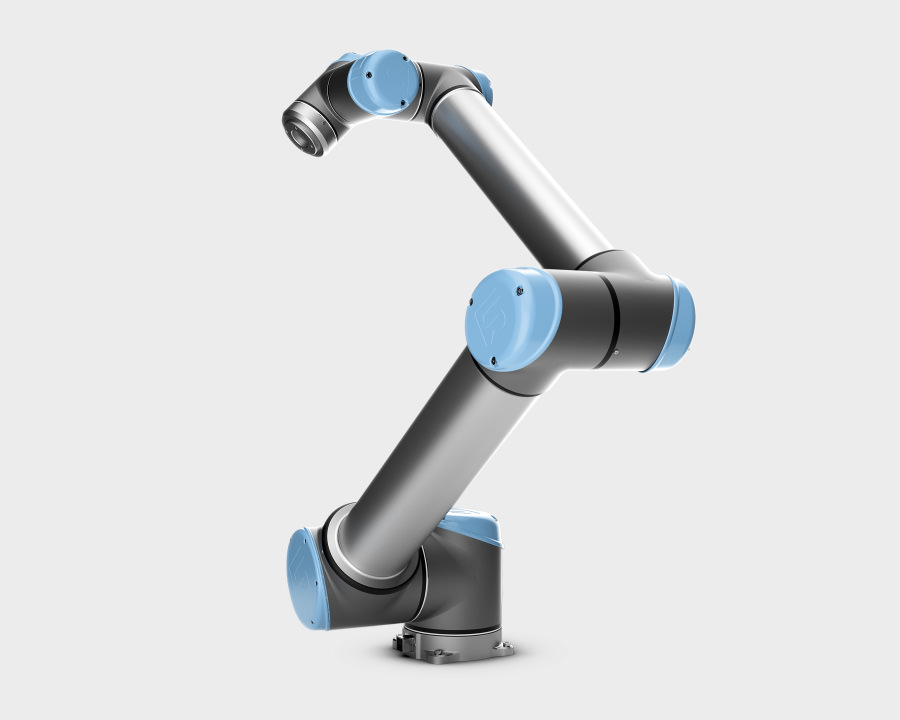
\includegraphics[width=1\textwidth]{UR10-UNIVERSAL-ROBOT}
    \caption{Robot Universal UR10.}
    \label{fig:UR10-UNIVERSAL-ROBOT}
\end{figure}


% Resumen
% ======================================================================
\begin{abstract}
    El presente documento presenta el proyecto final de la cátedra de Control y Sistemas de la Universidad Nacional de Cuyo.
    El objetivo del es aplicar los conocimientos, herramientas y habilidaddes adquiridas para realizar el modelado, análisis y simulación del control de posición para el accionamiento electromecánico de la primer articulación del robot Universal UR10 figura \ref{fig:UR10-UNIVERSAL-ROBOT}, un robot industrial tipo serie de 6 grados de libertad.

    El robot se modela como un sistema lineal variante en el tiempo (LTI), en donde se toma al momento de inercia como un parámetro variable de entrada al modelo de la planta, y se utiliza un tipo de controlador PID junto con la técnica de planificación de ganancias (en inglés: gain scheduling) para lograr el correcto seguimiento de consignas y rechazo de perturbaciones.

    Además, se incluye ruido de proceso en las variables de estado de la planta, y el modelado de un encoder absoluto ruidoso a la salida del sistema. Y luego se utiliza el filtro de Kalman con el objetivo de mitigar el ruido y obtener la estimación más óptima posible de la posición angular de salida que se retroalimenta al controlador.

    Finalmente el controlador PID, junto con el sensor y el filtro de Kalman, son modelados en el tiempo discreto con representación en punto fijo.
\end{abstract}


% Secciones
% ======================================================================

\section{INTRODUCCIÓN}
\label{sec:INTRODUCCIÓN}

Los brazos robóticos de varios eslabones en serie, llamados robots serie, poseen un Subsistema Mecánico Fuertemente No Lineal. Esto es debido a que, para cada articulación del robot, la posición (y también la velocidad y aceleración) de las demás articulaciones influyen en su dinámica.
Por otro lado, un controlador PID es una técnica de control lineal, por lo que en principio solo es aplicable a sistemas lineales.

Ahora bien, en el presente proyecto, se pretende aplicar un control PID para mover la articulación de la base del robot. Esto es justamente para poder analizar la viabilidad y las complejidades que surjan al tratar de aplicar dicho tipo de control a un sistema fuertemente no lineal, además de obtener resultados ya sean positivos o negativos, para ganar experiencia acerca de las ventajas y desventajas que se tienen respecto a otros métodos de control.

Para controlar un sistema no lineal, con la estratagia de control PID, básicamente se puede proceder de dos formas:

\begin{itemize}
    \item 1) LINEALIZANDO EL SISTEMA: Si el sistema es no lineal pero está cerca de ser lineal, es decir si se pueden despreciar sus no linealizades, obteniendo un modelo que se corresponda con el real dentro de una tolerancia dada por la aplicación.

    \item 2) UTILIZANDO PLANIFICACIÓN DE GANANCIAS (GAIN SCHEDULING): Ahora, si las no linealidas son demasiadas, una aproximación común es aplicar la estrategia llamada planificación de ganancias. En esta estrategia de control, básicamente primero se debe linealizar el sistema no lineal alrededor de diferentes puntos de operación, definidos de manera distribuida para todo el espectro en el que puede cambiar los parámetros y/o el comportamiento del sistema. Y luego, se crea una familia de controladores PID uno para cada punto, y se ajusta cada uno de ellos para que sea óptimo en su punto de operación. Finalmente, se hace que, de forma automática, el sistema de control alterne entre estos modelos lineales mientras se opera el sistema de tal forma de tener el mejor control lineal en cada punto donde se opere.
    Para un sistema que tiene un comportamiento diferente en distintas regiones operativas, (es decir, para un sistema no lineal), dicha estrategia de control será subóptima. Esta suboptimalidad puede ser tan leve que pase desapercibida, o podría ser lo suficientemente grave como para hacer que sea inviable aplicarlo al sistema real, por lo que se evaluará su optimalidad.
\end{itemize}

Como un robot serie posea grandes no linealidades, en el proyecto se aplicará la estrategía de gain scheduling.

El resultado esperado del proyecto es lograr manipular correctamente la dinámica del robot, de forma tal que se obtenga a cada instante de tiempo la posición angular deseada de su primer articulación, y tal que se mantenga una respuesta aceptable ante pertubaciones externas de torque en la carga mecánica del robot.



% ======================================================================
\section{DESARROLLO}
\label{sec:DESARROLLO}
% ======================================================================

\subsection{MODELO DE LA PLANTA}
\label{sec:MODELO DE LA PLANTA}

Como planta del proyecto, se optó por elegir al robot UR10, y se lo escogió debido a que sus características, resultan ser adecuadas para luego trabajar con el mismo en el Proyecto Final de Carrera.

\subsubsection{Software De Simulación}
\label{sec:Software De Simulación}

\paragraph{DESCRIPCIÓN GENERAL DEL SOFTWARE DE SIMULACIÓN}
\label{sec:DESCRIPCIÓN GENERAL DEL SOFTWARE DE SIMULACIÓN}
\hfill

El software elegido para llevar a cabo la simulación del robot UR10 es el llamado CoppeliaSim \cite{CoppeliaSim}, anteriormente conocido como V-REP (Virtual Robot Experimentation Platform). CoppeliaSim es un simulador de robótica de propósito general, un entorno de simulación de robots 3D que permite a los usuarios modelar, simular y visualizar el comportamiento de robots. Es multiplataforma (corre en Windows, Linux y MacOS); y sus principales campos de aplicación son la investigación y la educación en robótica. Originalmente fué desarrollado por la compañía japonesa Toshiba, y actualmente es mantenido activamente por Coppelia Robotics, una pequeña empresa Suiza.

CoppeliaSim, además ofrece soporte para una variedad de robots y sensores, lo que lo convierte en una elección popular para proyectos que involucran la simulación de sistemas robóticos. La capacidad de integrar y controlar robots de marcas reconocidas, como el robot serie UR10, hace que dicho software de simulación sea una opción valiosa para el presente proyecto.

Para realizar cálculos cinemáticos directos e inversos de los robots, utiliza un motor cinemático, y varias bibliotecas de simulación física (MuJoCo, Bullet, ODE, Vortex, Newton Game Dynamics) para realizar simulaciones de cuerpos rígidos. Los modelos y escenas se construyen ensamblando diversos objetos (mallas, articulaciones, varios sensores, nubes de puntos, árboles OC, etc.) en una estructura jerárquica como se muestra en la figura \ref{fig:Software CoppeliaSim}.

\begin{figure}[H]
    \centering
    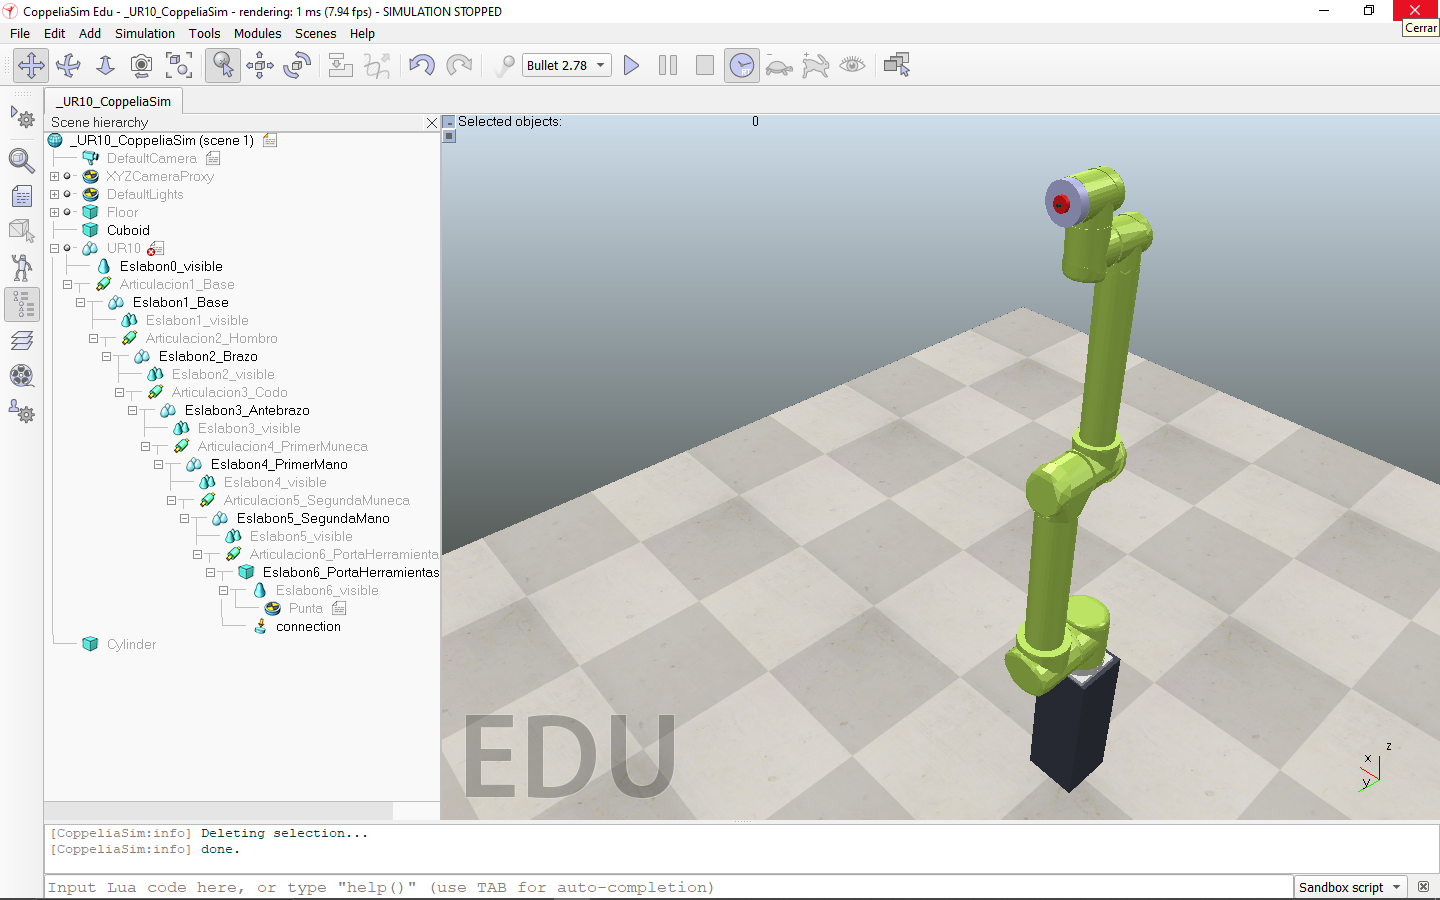
\includegraphics[width=1\textwidth] {Software CoppeliaSim}
    \caption{Software CoppeliaSim con robot UR10 en su configuración inicial (home), mostrando los archivos .STL de sus eslabones en color verde.}
    \label{fig:Software CoppeliaSim}
\end{figure}

CoppeliaSim está construido alrededor de una arquitectura de control distribuido que utiliza scripts en Python y Lua, o complementos (en inglés: plug-ins) en C/C++ que actúan como controladores individuales y síncronos. Controladores asincrónicos adicionales pueden ejecutarse en otro proceso, hilo o máquina a través de diversas soluciones de middleware (ROS, API remota, ZeroMQ) con lenguajes de programación como C/C++, Python, Java y MATLAB.


\subparagraph{Vinculación De Coppeliasim Con MATLAB/Simulink:}
\label{sec:Vinculación De Coppeliasim Con MATLAB/Simulink:}
\hfill

Particularmente, para llevar a cabo el proyecto, se utilizará CoppeliaSim en conjunto con MATLAB /Simulink. Esto es debido a que el control será implementado en Simulink, mientras que la simulación se implementará en CoppeliaSim.

Ambos softwares se comunicarán a través de una interfaz de programación de aplicaciones (siglas en inglés: API). CoppeliaSim ofrece más de 400 funciones API diferentes \cite{CoppeliaSim_API_Functions}.

La utilización de un software de simulación externo a MATLAB, como lo es CoppeliaSim, se dede a que la simulación del robot UR10 mediante la utilización de Simscape y el toolbox de robótica (robotics system toolbox) que ofrece MATLAB, resultó ser demasida lenta en obtenerse, llegando a tardar minutos para obtener pocos segundos de simulación. Incluso también siguió siendo inaceptable, luego de reducir el tamaño de los archivos .STL al reducir su cantidad de triángulos que forman el mallado, utilizando la aplicación Meshmixer \cite{Meshmixer}.

\begin{figure}[H]
    \centering
    \begin{minipage}{.5\textwidth}
        \centering
        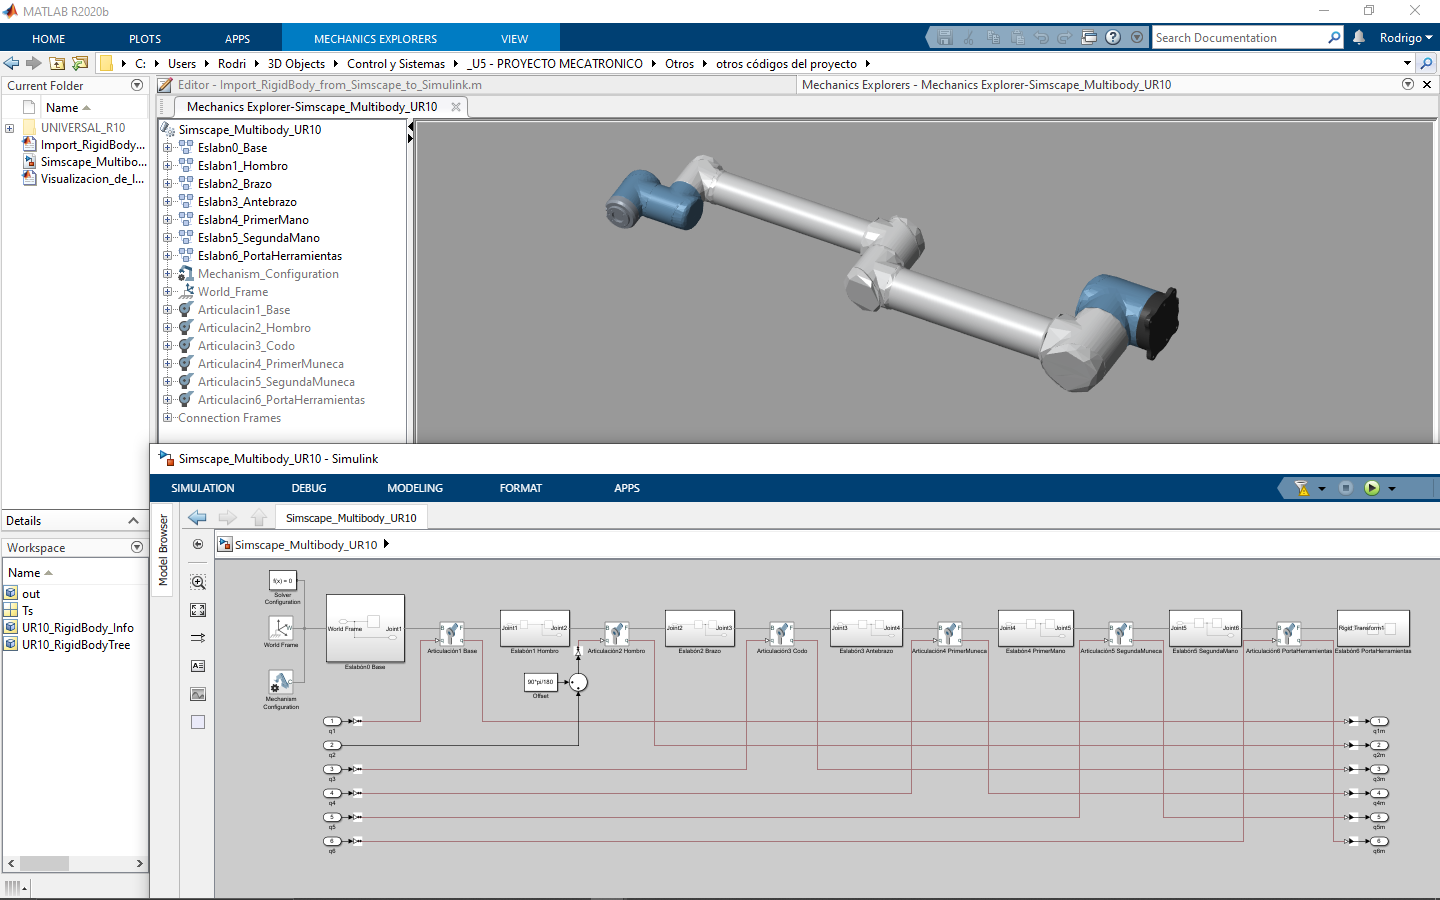
\includegraphics[width=1\textwidth]{Simscape}
        \caption{Simscape.}
        \label{fig:Simscape}
    \end{minipage}%
    \begin{minipage}{.5\textwidth}
        \centering
        \includegraphics[width=1\textwidth]{Toolbox de robótica de MATLAB}
        \caption{Toolbox de robótica de MATLAB.}
        \label{fig:Toolbox de robótica de MATLAB}
    \end{minipage}
    \caption{Diseño del robot UR10 en MATLAB Simscape, y su simulación utilizando el toolbox de robótica de MATLAB.}
\end{figure}


\paragraph{SIMULACIÓN CON COPPELIASIM}
\label{sec:SIMULACIÓN CON COPPELIASIM}
\hfill

Como primera medida de desarrollo del proyecto, se procedió a lograr mover todas las articulaciones del robot UR10 de la simulación en CoppeliaSim, a partir del pasaje de comandos de posición angular desde MATLAB/Simulink.

Para ello, en Simulink se necesitó hacer uso de una Función S de MATLAB de nivel 2 \cite{Level-2_MATLAB_S-Functions}. A dicha función se le colocó como entradas a las posiciones angulares, las cuales son ingresadas manualmente por medio de un panel con sliders creado en Simulink, o bien introduciendo los valores deseados de los ángulos en grados. Dichas posiciones angulares, dentro de la Función S de MATLAB de nivel 2 son transferidos a la simulación de CoppeliaSim mediante el uso de las funciones API para MATLAB que ofrece CoppeliaSim. Como se muestra en la figura \ref{fig:Movimiento del robot en CoppeliaSim, mediante panel en Simulink}, se logró mover exitosamente las articulaciones del robot.


\begin{figure}[H]
    \centering
    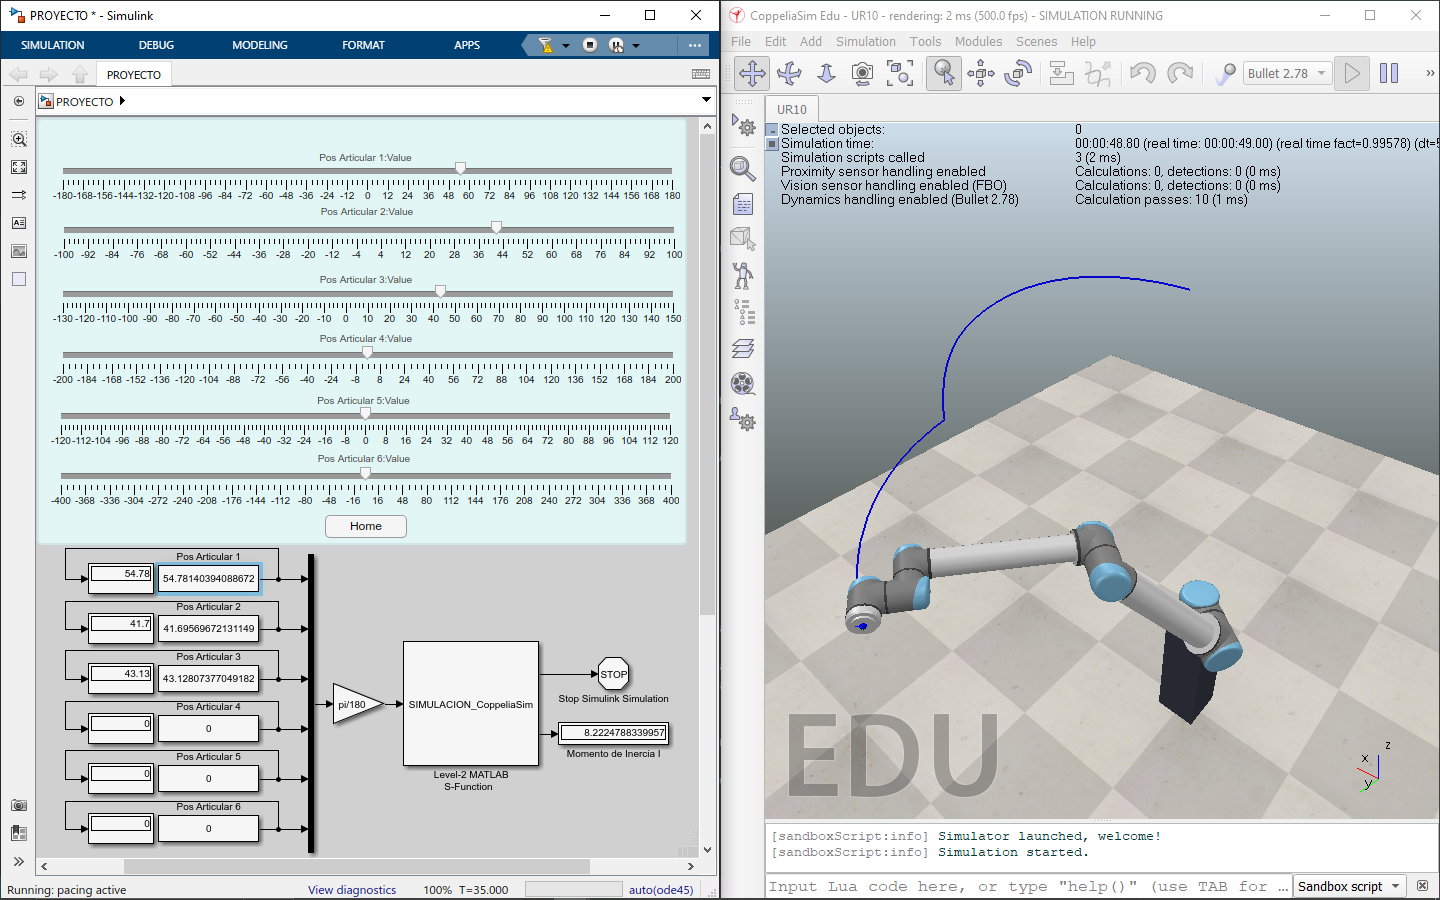
\includegraphics[width=1\textwidth] {Movimiento del robot en CoppeliaSim, mediante panel en Simulink}
    \caption{Movimiento del robot en CoppeliaSim, mediante panel en Simulink.}
    \label{fig:Movimiento del robot en CoppeliaSim, mediante panel en Simulink}
\end{figure}


\subsubsection{Descripción Del Robot:}
\label{sec:Descripción Del Robot:}

\paragraph{DESCRIPCIÓN GENERAL DEL ROBOT}
\label{sec:DESCRIPCIÓN GENERAL DEL ROBOT}
\hfill

El robot serie UR10, fabricado por la empresa danesa llamada: Universal Robots, posee una capacidad de carga de 10 kg, un alcance de 1300 mm, y brinda una repetibilidad de 0,1 mm. El UR10 es capaz de realizar una gran variedad de tareas que incluyen: paletización robótica, ensamblaje robótico, recogida y colocación automatizadas, manipulación de máquinas y embalaje, entre otras.

Además, es un robot del tipo Colaborativo, lo que significa que puede operar junto a los trabajadores sin necesidad de barreras de seguridad. Sus características de seguridad incluyen sensores de fuerza/par que previenen colisiones con los trabajadores.

Por otro lado, tiene la capacidad de ser programado por enseñanza, mediante su manipulación física de forma manual. Cabe mencionar que existe una versión mejorada el UR10, llamada UR10e, en donde la única diferencia es que la versión mejorada posee los sensores de fuerza/par incorporados, mayor precisión y una mejor interfaz.

\paragraph{ESPECIFICACIONES TÉCNICAS DEL ROBOT}
\label{sec:ESPECIFICACIONES TÉCNICAS DEL ROBOT}
\hfill

Las empresas dedicadas a dar productos y servicios de robótica, como lo es Universal Robots, debido a la competencia del mercado no brindan al público cierta información técnica específica de sus robots, para que estos no puedan ser replicados con facilidad. Por lo que suelen ser datos que no suelen estar disponibles públicamente de forma gratuita, por propiedad de los fabricantes, ya que se los considera información técnica confidencial.

Especialmente no fue fácil lograr encontrar los Parámetros Dinámicos (masas, momentos y productos de inercia) de los eslabones del robot, a pesar de realizar una extensa búsqueda de los mismos. La mayor dificultad se dió porque los valores que se encontraban no eran coherentes con sigo mismos y/o con el modelo del robot simulado en CoppeliaSim, probablemente por ser una versión distinta del mismo.

Para tener certeza acerca de que los valores de los parámetro dinámicos sean coherentes, se realizó el cálculo aproximado de los momentos de inercia de cada eslabón, a partir de su masa y una forma geométrica análoga simplificada utilizando las dimensiones geométricas del modelo CAD de CoppeliaSim. De esta forma, mediante prueba y error se lograron determinar cuales, de los valores de las masas y momentos de inercia de los eslabones que se disponen, son los que se corresponden correctamente con el modelo y versión del robot serie elegido para el proyecto. Dichos valores, se obtuvieron buscando información en un foro de Universal Robots, el cual posibilitó el acceso al repositorio de github \cite{Masas_y_Momentos_de_Inercia_de_github_de_Foro_UR}, de donde se terminaron tomando tales valores.

\subparagraph{Masa De Los Eslabones:}
\label{sec:Masa De Los Eslabones:}
\hfill \break
La tabla \ref{table:Masa de cada eslabón}, muestra la masa de cada eslabón en kg.
Como dato extra, la masa total del robot, la cual es igual a la suma de la masa de sus eslabónes, se ha obtenido de la hoja de datos de las epecificaciones técnicas del UR10 \cite{UR10_Especificaciones_Técnicas}, y es: $Mt = 28.9 kg$. Dicha masa total a sido útil para calcular la masa del eslabón base, ya que su valor no se encuentra, aunque dicha masa no es necesaria para la realización del proyecto en simulación.
\begin{table}[H]
\centering
\begin{tabular}{|l|lllllll|}
\cline{1-1}
\textbf{Eslabón}                                                                                  \\ \cline{1-8}
\textbf{Nombre}  & Base     & Hombro   & Brazo     & Antebrazo & 1er Mano  & 2da Mano  & 3er Mano \\ \cline{1-8}
\textbf{Número}  & 0        & 1        & 2         & 3         & 4         & 5         & 6        \\ \cline{1-8}
\textbf{Masa}    & 0.465 kg & 7.100 kg & 12.700 kg & 4.270 kg  & 2.000 kg  & 2.000 kg  & 0.365 kg \\ \cline{1-8}
\end{tabular}
\caption{\label{table:Masa de cada eslabón}Masa de cada eslabón.}
\end{table}


\subparagraph{Momentos Y Productos De Inercia:}
\label{sec:Momentos Y Productos De Inercia:}
\hfill \break
La tabla \ref{table:Momentos Y Productos De Inercia De Cada Eslabón}, muestra los momentos y productos de inercia, en unidades de $kg.m^2$, de cada eslabón del brazo robótico, respecto al centro de masa de cada una de ellos.
Dichos momentos y productos de inercia obtenidos del foro de universal robots tuvieron que ser reordenados, para que así coincidan con los ejes de los eslabones de robot en CoppeliaSim. % (Y además, solo a los Productos de Inercia que comenzaban con 4 decimales iguales a cero: 0.0000, los refiné a cero absoluto: 0.00000)
\begin{table}[H]
\begin{center}
\begin{tabular}{l|lll|lll|l}
\cline{2-7}
% & Jxx     & Jyy     & Jzz     & Jxy     & Jyz      & Jzx     &         \\ \cline{2-7}
% Eslabón 1 & 0.03529 & 0.03408 & 0.02156 & 0.00000 & -0.00425 & 0.00000 \\
% Eslabón 2 & 0.77068 & 0.76943 & 0.02814 & 0.00000 & -0.01561 & 0.00000 \\
% Eslabón 3 & 0.30928 & 0.30646 & 0.01014 & 0.00000 & 0.00916  & 0.00000 \\
% Eslabón 4 & 0.00296 & 0.00258 & 0.00222 & 0.00000 & -0.00024 & 0.00000 \\
% Eslabón 5 & 0.00296 & 0.00222 & 0.00258 & 0.00000 & -0.00024 & 0.00000 \\
% Eslabón 6 & 0.00040 & 0.00034 & 0.00041 & 0.00000 & 0.00000  & 0.00000 \\ \cline{2-7}
            & Jxx     & Jyy     & Jzz     & Jxy     & Jyz      & Jzx     &            \\ \cline{2-7}
Eslabón 1 & 0.03529 & 0.03408 & 0.02156 & 0.00000 & -0.00425 & 0.00000 & Hombro       \\
Eslabón 2 & 0.77068 & 0.76943 & 0.02814 & 0.00000 & -0.01561 & 0.00000 & Brazo        \\
Eslabón 3 & 0.30928 & 0.30646 & 0.01014 & 0.00000 & 0.00916  & 0.00000 & Antebrazo    \\
Eslabón 4 & 0.00296 & 0.00258 & 0.00222 & 0.00000 & -0.00024 & 0.00000 & 1er Mano  \\
Eslabón 5 & 0.00296 & 0.00222 & 0.00258 & 0.00000 & -0.00024 & 0.00000 & 2da Mano \\
Eslabón 6 & 0.00040 & 0.00041 & 0.00034 & 0.00000 & 0.00000  & 0.00000 & 3er Mano  \\ \cline{2-7}
\end{tabular}
\caption{\label{table:Momentos Y Productos De Inercia De Cada Eslabón}Momentos Y Productos De Inercia De Cada Eslabón.}
\end{center}
\end{table}


\subparagraph{Centro De Masa De Cada Eslabón:}
\label{sec:Centro De Masa De Cada Eslabón:}
\hfill \break
La tabla \ref{table:Centro De Masa De Cada Eslabón}, muestra la posición, en metros, de los centros de masa (CM) de cada eslabón, los cuales serán útiles a la hora de calcular el momento de inercia de la primer articulación del robot. Como se explica en la sección \ref{sec:Cálculo Del Momento De Inercia Equivalente:}, las coordenadas de dichas posiciones se encuentran referenciadas a la trama móvil de cada eslabón. Dichos valores de coordenadas fueron obtenidos de la simulación en CoppeliaSim.
\begin{table}[H]
\begin{center}
\begin{tabular}{l|lll|lll|l}
\cline{2-4}
          & CMx     & CMy      & CMz      &              \\ \cline{2-4}
Eslabón 1 & 0.00000 &  0.00587 & -0.00355 & Hombro       \\
Eslabón 2 & 0.00000 & -0.00076 & -0.03733 & Brazo        \\
Eslabón 3 & 0.00000 &  0.00388 & -0.01720 & Antebrazo    \\
Eslabón 4 & 0.00000 & -0.00304 &  0.00213 & 1er Mano  \\
Eslabón 5 & 0.00000 &  0.00213 & -0.00302 & 2da Mano \\
Eslabón 6 & 0.00000 & -0.00375 & -0.00018 & 3er Mano  \\ \cline{2-4}
\end{tabular}
\caption{\label{table:Centro De Masa De Cada Eslabón}Centro De Masa De Cada Eslabón.}
\end{center}
\end{table}


% ### LÍMITES ARTICULARES:
\subparagraph{Límites Articulares:}
\label{sec:Límites Articulares:}
\hfill \break
La tabla \ref{table:Límites Articulares, Velocidades Angulares Máximas y Torques Máximos de las articulaciones} muestra el rango articular y los límites articulares dentro de los cuales se puede desplazar cada articulación del robot.

% ### MÁXIMAS VELOCIDADES ANGULARES DE LAS ARTICULACIONES:
\subparagraph{Máximas Velocidades Angulares De Las Articulaciones:}
\label{sec:Máximas Velocidades Angulares De Las Articulaciones:}
\hfill \break
La tabla \ref{table:Límites Articulares, Velocidades Angulares Máximas y Torques Máximos de las articulaciones} muestra las velocidades angulares máximas que puede alcanzar cada articulación del robot. Particularmente, nos interesa solo la máxima velocidad angular de la articulación base.

% ### MÁXIMOS TORQUES DE LAS ARTICULACIONES:
\subparagraph{Máximos Torques De Las Articulaciones:}
\label{sec:Máximos Torques De Las Articulaciones:}
\hfill \break
La tabla \ref{table:Límites Articulares, Velocidades Angulares Máximas y Torques Máximos de las articulaciones}, también muestra muestra los máximos torques que el robot podría entregar en la aplicación, los cuales fueron obtenidos de la página web de Universal Robots \cite{Torques_Máximos}. Dichos torques corresponden a la posición articular más desfavorable, es decir la que máyor torque requiera, y con la máxima carga de 10 kg. Particularmente, nos interesa solo el máximo torque de la articulación base.

\begin{table}[H]
    \centering
    \begin{tabular}{|l|llllll|}
    \cline{1-1}
    \textbf{Articulación}                                                                             \\ \cline{1-7}
    \textbf{Nombre}    & Base       & Hombro     & Codo       & 1er Muñeca & 2da Muñeca  & 3ra Muñeca \\ \cline{1-7}
    \textbf{Número}    & 1          & 2          & 3          & 4          & 5           & 6          \\ \cline{1-7}
    \textbf{Rango}     & 360°       & 200°       & 280°       & 400°       & 240°        & 800°       \\ \cline{1-7}
    \textbf{Límites}   &[-180, 180] &[-100, 100] &[-130, 150] &[-200, 200] &[-120, 120]  &[-400, 400] \\ \cline{1-7}
    \textbf{Máx. Vel.} & 120°/s     & 120°/s     & 180°/s     & 180°/s     & 180°/s      & 180°/s     \\ \cline{1-7}
    % Por otro lado, la MÁXIMA VELOCIDAD LINEAL TÍPICA DE LA HERRAMIENTA suele ser:  1 m/s
    \textbf{Máx. Torque} & 330 Nm   & 330 Nm     & 150 Nm     & 56 Nm      & 56 Nm       & 56 Nm     \\ \cline{1-7}
    \end{tabular}
    \caption{\label{table:Límites Articulares, Velocidades Angulares Máximas y Torques Máximos de las articulaciones}Límites Articulares, Velocidades Angulares Máximas y Torques Máximos de las articulaciones.}
\end{table}
%  Velocidad Angular Máxima de la Base = 120°/s = 20 RPM



\subsubsection{Simplificaciones del Modelo}
\label{sec:Simplificaciones del Modelo}

\paragraph{Control Monoarticular}
\label{sec:Control Monoarticular}
\hfill

Las aplicaciones de los robots serie, implican que estos muevan dos o más de sus articulaciones simultáneamente, mediante un Método de Control Multiarticular. Pero, en tal caso se tiene un sistema de múltiples entradas y múltiples salidas (MIMO) con 6 variables de entrada y 6 de salida, y para utilizar un control de tipo PID como se propuso en la introducción, entonces se tendría que poder realizar el tunning de los parámetros a 6 Controladores PID, uno por cada articulación.

Esto resulta prácticamente inviable, ya que al lograr tunear un primer PID correspondiente a una de las variables, y comenzar a tunear otro, hay que volver a tunear el primero. Esto es, ya que una variable influencia en la respuesta de la otra variable, debido al que existe un acoplamiento entre las mismas. Entonces se tendría que estar modificando permanentemente ambos controladores PID, hasta que en algún momento funcione todo bien y no se sigan modificando.

Y si tunear dos Controladoes PID es complicado, tunear 6 Controladores PID resulta prácticamente imposible, ya que al modificar los parámetros de uno, se deben modificar los parámetros de los otros 5, hasta lograr cumplir con los objetivos de control.
Por este motivo, no sería factible utilizar el control PID, sino que se necesitaría hacer uso de otra técnica de control, como una técnica de control no lineal con realimentación completa del vector de estados.

Por ello, se procede a simplificar la aplicación del robot, al suponer que en el movimiento de una de las articulaciones del mismo, las demás 5 articulaciones permanecen inmóviles. En otras palabras: se simplifica el modelo al consider un Método de Control Monoarticular, en el que cada articulación del robot se controla de manera independiente.

Si bien, el control multiarticular es el que verdaderamente se utiliza en las aplicaciones reales, el control monoarticular es un enfoque común para probar un robot. Esto es debido a que, el control monoarticular al considerar un controlador independiente para cada articulación, provoca que se independicen las articulaciones entre sí. Por lo que no se necesitan tener en cuenta los acoplamientos dinámicos que existen entre las articulaciones, ni las vibraciones que introduce el movimiento de cada una de ellas a las demás, lo que simplifica bastante el control haciéndolo un buen método de control inicial para probar un robot.

Además, dicha simplificación hace que el modelo del sistema se acerque un poco a ser lineal.

\paragraph{Sin Deformaciones Elásticas}
\label{sec:Sin Deformaciones Elásticas}
\hfill

Como otra simplificación, y debido a las características de sus materiales, se considera que el robot no posee deformaciones elásticas, es decir, con piezas totalmente rígidas.


\paragraph{Subsistema Térmico}
\label{sec:Subsistema Térmico}
\hfill

\hfill

El subsistema térmico de la planta no debería ser despreciado debido a la relativamente alta potencia que requiere el robot, ya que se podría tener repercusiones importantes en el desempeño y seguridad de la planta real. Pero se ha decidido no considerarlo en principio, por no ser demasiado relavante en los objetivos del proyecto, y para así poder dedicarle más tiempo a otros temas más relevantes del mismo.

\paragraph{Cantidad de Sensores}
\label{sec:Cantidad de Sensores}
\hfill

\hfill

Al tratarse de un robot colaborativo, como seguridad ante colisiones de cualquier tipo, estos poseen sensores de fuerza/par. Además, como los cobots trabajan junto a humanos, necesitan de una retroalimentación de doble encoder para aumentar la detección de fuerza y monitorear la consistencia, suavidad, y precisión.
%  Doble-Encoder. URL: %https://www.youtube.com/watch?v=EaaSNB8vfKU&t=87s.
Pero en el proyecto toma la simplificación de considerar solo un sensor de posición absoluta para la articulación controlada.

% \paragraph{Modulador De Tensión}
% \label{sec:Modulador De Tensión}
% \hfill

% [[[[El modulador de tensión se lo considera como BLOQUE ABSTRACTO qué tiene una GANANCIA APROXIMADAMENTE UNITARIA y un ancho de banda muy grande (comparado con el ancho de banda que va a quedar nuestro controlador, o sea donde "van a estar" los polos de lazo cerrado del controlador de movimiento), entonces lo podemos considerar como MODULADOR IDEAL. """BORARRR:(Y del mismo modo consideramos ideales a los sensores)""". Con lo que tenemos un acceso directo entre la señal de control de tensión y la tensión efectiva. Es una linealización y una aproximación lo que estamos haciendo pero para los efectos de diseño esto es totalmente válido.]]]]



\subsubsection{Elaboración del Modelo:}
\label{sec:Elaboración del Modelo:}

Como se explicará en la sección \ref{sec:CONTROLADOR} donde se diseña al controlador, la primer etapa para implementar la técnica de control gain scheduling, es obtener un modelo lineal de la planta a controlar.
Desde el punto de vista de transformaciones de energía, el modelo del sistema consiste de tres subsistemas: el subsistema mecánico, el subsistema electromagnético y el subsistema térmico. Aunque como se menconó el subsistema térmico no será tenido en cuenta.

\subsubsection{SUBSISTEMA MECÁNICO:}
\label{sec:SUBSISTEMA MECÁNICO:}

El subsistema mecánico se encuentra formado por el conjunto: articulación-reductor-motor; o en otras palabras, se encuentra formado por la carga mecánica, la caja reductora y la máquina eléctrica.

\paragraph{\textbf{CARGA MECÁNICA}}
\label{sec:CARGA MECÁNICA}
\hfill

\hfill

Para obtener el modelo matemático lineal del comportamiento no lineal de la carga mecánica del brazo robótico, se considera que
la carga posee un comportamiento lineal, mediante el uso de, en principio, los siguientes dos parámetros equivalentes variables:
\begin{itemize}
    \item Momento de inercia equivalente (variable):
    \\ Al cambiar el ángulo de alguna otra articulación del robot, diferente a la primera, el momento de inercia respecto al eje de rotación que experimenta la primer articulación varia, y se toma como un parámetro variable.

    \item Amortiguamiento viscoso equivalente (variable):
    \\ Este amortiguamiento, además de involucrar al coeficiente constante de la fricción  propia de la articulación, también corresponde a una fricción ficticia, con la cual se logra involucrar de forma equivalente los efectos de las fuerzas centrífugas y de Coriolis que aparecen cuando se mueven las demás articulaciones.
\end{itemize}
Es decir, con dichos parámetros se obtendrá un modelo lineal de parámetros variables (LPV), en donde se tiene una incertidumbre en cuál es el valor de dichos parámetros, en función de cuál es el estado dinámico de las demás articulaciones.
Aunque, debido a la simplificación de considerar un método de control monoarticular, entonces al moverse la primera articulación, la velocidad y aceleración de las demás 5 articulaciones son siempre cero. Por ello, también sus fuerzas centrífugas y de Coriolis serán siempre nulas, y por lo tanto no se necesita el amortiguamiento ficticio viscoso equivalente variable. Es decir, que solo se necesita considerar como parámetro variable, al momento de inercia equivalente.

\hfill

\subparagraph{Cálculo Del Momento De Inercia Equivalente:}
\label{sec:Cálculo Del Momento De Inercia Equivalente:}

\hfill

\hfill

A continuación, se procede a obtener la fórmula matemática para el cálculo del momento de inercia equivalente respecto al eje de giro de la primer articulación del robot; momento de inercia que es variante en el tiempo, ya que depende de cuál sea la posición instantánea de las articulaciones superiores del robot.

Todos los cálculos nescesarios para la obtención de dicho momento de inercia, serán realizados dentro de la Función S de MATLAB de nivel 2, mencionada en la sección \ref{sec:SIMULACIÓN CON COPPELIASIM}, de tal forma de poderla actualizar en cada iteración.

Por otro lado, es aclaratorio mencionar que el eje de giro de la primer articulación del robot se lo colocó, en la simulación de CoppeliaSim, en las coordenadas absolutas X=0 e Y=0 con la finalidad de hacerlo colineal al eje Z absoluto de la escena de CoppeliaSim.

\hfill \break
Marcos De Referencia:
\begin{itemize}
    \item Marco De Referencia Absoluto:
        \\ Es el sistema de coordenadas fijo que se muestra en la esquina inferior derecha de las escenas de CoppeliaSim. Sus ejes se los denomina con las letras mayúsculas: X,Y y Z.
    \item Tramas De Las Mallas De Los Eslabones:
        \\ Estas son los marcos de referencia de los archivos .STL (mallas, del inglés: meshes) de los eslabones, que se encuentran fijos a los eslabones, y se mueven con él. Aunque el origen de coordenadas de estas tramas se encuentran relativamente cerca de los centros de masa de los eslabones, no coinciden, y su diferencia en posición no es despreciable.
\end{itemize}

% \textbf{Nomenclaturas:}
% \begin{description}
%     \item[PE:] Posiciones absolutas de las tramas de los Eslabónes.
%     \item[OE\_Q:] Orientaciones de los Eslabones, utilizando Cuaterniones.
%     \item[OE\_MR:] Orientaciones de los Eslabones, utilizando Matrices de Rotación.
%     \item[ME:] Masas de los Eslabónes.
%     \item[CME\_Mallas:] Centros de Masas respecto a las tramas de las Mallas de los Eslabones.
%     \item[CME\_Mundo] Centros de Masa de los Eslabónes, respecto al Mundo (posiciones absolutas).
%     \item[IE\_OL] Momento de Inercia de los Eslabones con respecto a un eje arbitrario OL
%     \item[I] Momento de Inercia Equivalente del robot, respecto del eje de rotación (eje vertical Z) de su primera articulación.
%     \item[IE] Momentos y Productos de Inercia de los Eslabones del robot.
%     \item[IE\_OL] Momentos de Inercia de los Eslabones del robot, respecto a un eje arbitrario OL.
% \end{description}

Como se observa en la ecuación \ref{eq:J_Z}, el momento de inercia $J_Z$ respecto del eje vertical Z de rotación de la primer articulación del robot, en una configuración genérica (fija) de sus articulaciones, es igual a la suma de los momentos de inercia $J_{Ei_Z}$ de cada i-eslabón respecto al eje Z. En donde, como muestra la ecuación \ref{eq:J_Ei_Z}, el momento de inercia $J_{Ei_Z}$ del eslabón-i es igual al momento de inercia $J_{Ei_{Z_{CM}}}$ del eslabón respecto al eje $Z_{CM}$ que es paralelo al eje Z y que pasa por su Centro de Masa (CM); más la masa del eslabón multiplicada por el cuadrado de la distancia $D_{Ei_{CM_{XY}}}$ del eslabón-i, entre el eje Z absoluto, y su CM, a lo largo del plano XY.

\begin{align} \label{eq:J_Z}
	J_Z=\sum_{i=1}^{i=6}J_{Ei_Z}
\end{align}

\begin{align} \label{eq:J_Ei_Z}
    J_{Ei_Z}=J_{Ei_{Z_{CM}}}+M_{Ei}.(D_{Ei_{(Z-CM)_{XY}}})^2
\end{align}

Entonces, para poder realizar dicho cálculo de forma automática en cada iteración, para cualquier configuración de las articulaciones del robot, se debe poder obtener en cada iteración:
\begin{itemize}
    \item El momento de inercia $J_{Ei_{Z_{CM}}}$ de cada i-eslabón.
    \item La distancia $D_{Ei_{(Z-CM)_{XY}}}$ de cada i-eslabón.
\end{itemize}


\hfill

Cálculo Del Momento De Inercia $J_{Ei_{Z_{CM}}}$:

\hfill

El problema de obtener el Momento De Inercia $J_{Ei_{Z_{CM}}}$ del eslabón-i respecto al eje Z absoluto para una orientación arbitraria del eslabón, por tratarse de un problema de estática, es equivalente al problema de considerar al eslabón fijo y obtener su Momento De Inercia respecto a un eje Z con orientación arbitraria.


El momento de inercia $J_{OL}$ de un cuerpo (fijo) con respecto a un eje arbitrario OL, está dado por la ecuación (9.46) del libro de mecánica racional de estática \cite{beermecanica}, mostrada en el presente documento en la ecuación \ref{eq:J_OL}:

\begin{align} \label{eq:J_OL}
    J_{Ei_{Z_{CM}}} = J_{OL} = J_X.\lambda_X^2+J_Y.\lambda_Y^2+J_Z.\lambda_Z^2-2.J_{XY}.\lambda_X.\lambda_Y-2.J_{YZ}.\lambda_Y.\lambda_Z-2.J_{ZX}.\lambda_Z.\lambda_X
\end{align}

En donde:
\begin{itemize}
    \item Jxx, Jyy, Jzz, Jxy, Jyz e Jzx son respectivamente los momentos y productos de inercia del eslabón-i, dados por la tabla \ref{table:Momentos Y Productos De Inercia De Cada Eslabón}, correspondientes a los ejes $x_{CM}$, $y_{CM}$ y $z_{CM}$ que pasan por su CM y que son paralelos a la trama fija de la malla de dich o eslabón.
    \item $\lambda$ es un vector unitario localizado a lo largo del eje OL, y sus componentes $\lambda_X$, $\lambda_Y$ y $\lambda_Z$ representan los cosenos directores de dicho eje arbitrario.
\end{itemize}

Dichos cosenos directores se obtienen en cada iteración de la tercera columna de la matriz de rotación del eslabón, la cual se debería obtener desde CoppeliaSim. Pero las Funciones API del simulador, no incluyen el pasaje de las matrices de rotación a MATLAB \cite{API_Functions_MATLAB} \cite{MR_to_MATLAB}, solo permite el pasaje de las orientaciones de los objetos mediante el uso de ángulos de Euler o de Cuaterniones. Y debido a que los Cuaterniones son el mejor método de representación de las rotaciones, ya que no posee problemas como el bloqueo del cardán (en inglés: gimbal lock) que presentan los ángulos de Euler, se eligió realizar el pasaje de las orientaciones de CoppeliaSim a MATLAB mediante el uso de cuaterniones \cite{Cuaterniones}. En MATLAB, las orientaciones son recibidas dentro de la Función S de MATLAB de nivel 2, haciendo usa de la API. Dentro de esta función S de nivel 2 se convierten las orientaciones de cuaterniones a matrices de rotación $MR_{Ei}$, de donde se obtienen los valores de $\lambda_X$, $\lambda_Y$ y $\lambda_Z$, y se realiza el cálculo del momento de inercia $J_{Ei_{Z_{CM}}}$ con la ecuación \ref{eq:J_Ei_Z_CM}, equivalente a la ecuación \ref{eq:J_OL}.

\begin{align} \label{eq:J_Ei_Z_CM}
    \begin{aligned}
    J_{Ei_{Z_{CM}}} =
    & J_X.MR_{Ei_{[3,1]}}^2+J_Y.MR_{Ei_{[3,2]}}^2+J_Z.MR_{Ei_{[3,3]}}^2- \\
    & -2.J_{XY}.MR_{Ei_{[3,1]}}.MR_{Ei_{[3,2]}}-2.J_{YZ}.MR_{Ei_{[3,2]}}.MR_{Ei_{[3,3]}}-2.J_{ZX}.MR_{Ei_{[3,3]}}.MR_{Ei_{[3,1]}}
    \end{aligned}
\end{align}

\hfill

Cálculo De La Distancia $D_{Ei_{(Z-CM)_{XY}}}$:

\hfill

Como el eje Z se encuentra siempre en la posición X=0 e Y=0, entonces la distancia $D_{Ei_{CM_{XY}}}$ es simplemente la distancia absoluta al CM del eslabón-i en el plano XY. La cual se obtiene aplicando pitágoras \ref{eq:D_Ei_CM_XY} a las coordenadas absolutas del centro de masa $CM_{Ei_X}$ y $CM_{Ei_Y}$ del eslabón-i:

\begin{align} \label{eq:D_Ei_CM_XY}
    D_{Ei_{CM_{XY}}} = \sqrt{CM_{Ei_X}^2+CM_{Ei_Y}^2}
\end{align}

Ahora las coordenadas $CM_{Ei_X}$ y $CM_{Ei_Y}$ no son brindadas por CoppeliaSim. Por lo que, para la obtención de dichas coordenadas absolutas de un eslabón-i, se tuvieron que sumar \ref{eq:CM_Ei_X y CM_Ei_Y} respectivamente las coordenadas X e Y de la posición absoluta del origen de coordenadas de la trama de la malla del eslabón-i $PT_{Ei_X}$ y $PT_{Ei_Y}$, con las distancias $D_{Ei_{(T-CM)_X}}$ y $D_{Ei_{(T-CM)_X}}$ respectivamente a lo largo de los ejes X e Y absolutos entre la trama del eslabón y su CM.

\begin{subequations} \label{eq:CM_Ei_X y CM_Ei_Y}
	\begin{align}
        \label{eq:CM_Ei_X}   CM_{Ei_X}=PT_{Ei_X}+D_{Ei_{(T-CM)_X}} \,,\\
        \label{eq:CM_Ei_Y}   CM_{Ei_Y}=PT_{Ei_Y}+D_{Ei_{(T-CM)_Y}} \,
	\end{align}
\end{subequations}

En donde:
\begin{itemize}
    \item Las coordenadas X e Y de la posición absoluta del origen de coordenadas de la trama de la malla del eslabón-i $PT_{Ei_X}$ y $PT_{Ei_Y}$, son recibidas dentro de la Función S de MATLAB de nivel 2, las cuales son obtenidas desde CoppeliaSim haciendo usa de la API.
    \item las distancias $D_{Ei_{(T-CM)_X}}$ y $D_{Ei_{(T-CM)_X}}$ son calculadas a partir de: las coordenadas del centro de masa del eslabón-i relativas a su trama $CM_{Ei_{Tx}}$, $CM_{Ei_{Ty}}$ y $CM_{Ei_{Tz}}$, junto con las orientaciones de los eslabones mediante el respectivo uso de la primer ($MR_1$) y segunda ($MR_2$) columnas de la matriz de rotación del eslabón. Tal y como se muestra en la ecuación \ref{eq:D_Ei_(T-CM)_X y D_Ei_(T-CM)_X}.
\end{itemize}

\begin{subequations} \label{eq:D_Ei_(T-CM)_X y D_Ei_(T-CM)_X}
	\begin{align}
        D_{Ei_{(T-CM)_X}} = CM_{Ei_{Tx}}.MR_{Ei_{[1,1]}} + CM_{Ei_{Ty}}.MR_{Ei_{[1,2]}} + CM_{Ei_{Tz}}.MR_{Ei_{[1,3]}} \,,
        \\
        D_{Ei_{(T-CM)_Y}} = CM_{Ei_{Tx}}.MR_{Ei_{[2,1]}} + CM_{Ei_{Ty}}.MR_{Ei_{[2,2]}} + CM_{Ei_{Tz}}.MR_{Ei_{[2,3]}} \,
    \end{align}
\end{subequations}

En donde:
\begin{itemize}
    \item Los valores de las coordenadas del centro de masa del eslabón-i relativas a su trama $CM_{Ei_{Tx}}$, $CM_{Ei_{Ty}}$ y $CM_{Ei_{Tz}}$ se encuentran en la tabla \ref{table:Centro De Masa De Cada Eslabón}.
\end{itemize}

Cabe mencionar que la entrada de los parámetros de las masas, coordenadas de los centros de masa (respecto a las tramas de los eslabones) y momentos y productos de inercia, a la función s de MATLAB de nivel 2, se a realizado ingresándolos mediante el cuadro de diálogo de los parámetros de bloque \cite{Pass_Dialog_Parameters} de la función S.
%COMO ESTABA y COMO ESTÁ TAMBIÉN AHORAAAAA:
% [7.100, 12.700, 4.270, 2.000, 2.000, 0.365],
% [ 0.00000,  0.00587, -0.00355;
%   0.00000, -0.00076, -0.03733;
%   0.00000,  0.00388, -0.01720;
%   0.00000, -0.00304,  0.00213;
%   0.00000,  0.00213, -0.00302;
%   0.00000, -0.00375, -0.00018],
% [0.03529 0.03408 0.02156   0.00000 -0.00425  0.00000;
%  0.77068 0.76943 0.02814   0.00000 -0.01561  0.00000;
%  0.30928 0.30646 0.01014   0.00000 +0.00916  0.00000;
%  0.00296 0.00258 0.00222   0.00000 -0.00024  0.00000;
%  0.00296 0.00222 0.00258   0.00000 -0.00024  0.00000;
%  0.00040 0.00041 0.00034   0.00000  0.00000  0.00000]

Así, se ha logrado obtener el Momento de Inercia Equivalente Variable $J_Z$, el cual se brinda como salida de la función S de MATLAB de nivel 2, tal y como se puede apreciar en la figura \ref{fig:Movimiento del robot en CoppeliaSim, mediante panel en Simulink}.

Particularmente, se obtuvo el valor máximo y mínimo del $J_Z$, dado que serán de utilidad a la hora de aplicar el método de control de planificación de ganancias. Dichos valores extremos se dan para las posiciones articulares mostradas en las figuras \ref{fig:Máximo Momento de Inercia} y \ref{fig:Mínimo Momento de Inercia}, y son los mostrados en las igualdades \ref{eq:J_Z_máx y J_Z_mín}:

\begin{subequations} \label{eq:J_Z_máx y J_Z_mín}
	\begin{align}
        J_{Z_{\text{mín.}}} =  0,56982 ~[kg.m^2] \,, \text{Posición articular: [-,90°,0,0,0,-]}
        \\
        J_{Z_{\text{máx.}}} = 12,54696 ~[kg.m^2] \,, \text{Posición articular: [-,0,0,0,120°,-]}
    \end{align}
\end{subequations}

\begin{figure}[H]
    \centering
    \begin{minipage}{.5\textwidth}
        \centering
        \includegraphics[width=0.99\textwidth]{Máximo Momento de Inercia}
        \caption{Máximo Momento de Inercia.}
        \label{fig:Máximo Momento de Inercia}
    \end{minipage}%
    \begin{minipage}{.5\textwidth}
        \centering
        \includegraphics[width=0.99\textwidth]{Mínimo Momento de Inercia}
        \caption{Mínimo Momento de Inercia.}
        \label{fig:Mínimo Momento de Inercia}
    \end{minipage}
\end{figure}



\hfill
\subparagraph{\textbf{Obtención Del Modelo De La Carga Mecánica:}}
\label{sec:Obtención Del Modelo De La Carga Mecánica}

\hfill

\hfill

Una vez obtenido nuestro parámetro equivalente variable $J_Z$, se procede con la obtención del modelo de la carga mecánica.

En la Figura \ref{fig:Descripción esquemática clásica de una transmisión} se muestra la descripción esquemática clásica de una transmisión que representa a la articulación del robot, figura obtenida de \cite{arenas2023virtual}. En donde $J_l=J_Z$ es el momento de inercia calculado, y se encuentra referido al eje de salida de la caja reductora de la primer articulación.

\begin{figure}[H]
    \centering
    \includegraphics[width=0.8\textwidth]{Descripción esquemática clásica de una transmisión}
    \caption{Descripción esquemática clásica de una transmisión.}
    \label{fig:Descripción esquemática clásica de una transmisión}
\end{figure}

Aplicando la Segunda Ley de Newton, se tiene que el momento de inercia multiplicado por la aceleración angular, es igual a la sumatoria de torques aplicados sobre la carga mecánica. Con lo que el modelo simplificado equivalente de la carga mecánica, con el parámetro equivalente variable $J_l$ está dado por:

\begin{subequations} \label{eq:J_l y theta_l}
    \begin{align}
        & \label{eq:J_l}         J_l.\ {\dot{\omega}}_l\left(t\right)=T_q\left(t\right)-b_l.\omega_l(t)-T_l(t)
        \\
        & \label{eq:theta_l(t)}     \frac{{\ \ d\theta}_l\left(t\right)}{dt}\left(t\right)=\omega_l\left(t\right)\Leftrightarrow{\ \ \theta}_l\left(t\right)=\int_{0}^{t}{\omega_l\left(\xi\right).d\xi}+\theta_l\left(0\right)
    \end{align}
\end{subequations}

Donde el término $b_l.\omega_l(t)$ representa la fricción propiamente dicho, de la carga de la articulación base.

Siendo:
\begin{description}
    \item[$J_l:$] Momento de inercia equivalente (variable), de la carga.
    \item[$b_l:$] Amortiguamiento viscoso equivalente de la carga.
    \item[$\theta_l(t):$] Ángulo del eje de salida de la caja reductora.
    \item[$\omega_l(t):$] Velocidad angular del eje de salida de la caja reductora.
    \item[$T_q(t):$] Torque de salida de la caja reductora.
    \item[$T_l(t):$] Torque resistente proporcionado por la carga externa, (o torque de carga).
\end{description}



\begin{subequations} \label{eq:Valor de b_l y de b_l}
    \begin{align}
        & \label{eq:Valor de b_l}  b_l=1,5\times10^{-5}\ \ \frac{N.m}{rad/s}
        \\
        & \label{eq:Valor de T_l}  T_l(t)=(0\pm330)\ N.m
    \end{align}
\end{subequations}






\paragraph{CAJA REDUCTORA}
\label{sec:CAJA REDUCTORA}
\hfill

\hfill


La caja reductora de cada una de las seis articulaciones del brazo robótico corresponde a un reductor armónico \ref{fig:Reductor Armónico}.

\begin{figure}[H]
    \centering
    \includegraphics[width=0.8\textwidth]{Reductor Armónico}
    \caption{Reductor Armónico.}
    \label{fig:Reductor Armónico}
\end{figure}

Estas unidades se caracterizan por tener altas relaciones de transmisión, lo que las hace compactas y livianas, y por tener cero juego “backlash” entre los engranajes, lo que las hace muy precisas.
Por no tener “backlash”, y debido a la alta precisión que maneja el robot, y a la simplificación \ref{sec:Sin Deformaciones Elásticas} de considerarlo sin deformaciones elásticas, entonces se considera al reductor armónico como un acoplamiento rígido sin elasticidad torsional. Por lo tanto, su modelo se lo puede expresar con un único grado de libertad:

\begin{subequations} \label{eq:theta_l, omega_l y T_q}
    \begin{align}
        & \label{eq:theta_l}   \theta_l(t)=\frac{\theta_m(t)}{r}
        \\
        & \label{eq:omega_l}   \omega_l(t)=\frac{\omega_m(t)}{r}
        \\
        & \label{eq:T_q}   T_q(t)=r.T_d(t)
    \end{align}
\end{subequations}

Donde:
\begin{description}
    \item[$\omega_m\left(t\right):$] Velocidad angular (geométrica) del motor.
    \item[r:] Relación de reducción.
    \item[$T_d(t):$] Torque resistente proporcionado por la caja reductora.
\end{description}

\begin{align} \label{eq:Valor de r}
	r = 160\text{}{:}1
\end{align}

Si no se considerara dicha simplificación de acoplamiento idealmente rígido, entonces la caja reductora dividiría al subsistema mecánico en dos partes, cada una con un grado de libertad rotacional distinto; impidiendo su compactación o simplificación en una única ecuación.


\paragraph{MÁQUINA ELÉCTRICA}
\label{sec:MÁQUINA ELÉCTRICA}
\hfill

\hfill


La información exacta acerca del tipo de motor utilizado en cada articulación del robot es conocimiento propietario de Universal Robots, y no se encuentra a disposición.

\subparagraph{Selección del Motor:}
\label{sec:Selección del Motor:}
\hfill

\hfill

Para el desarrollo del proyecto, se considera que el UR10 posee en sus articulaciones motores de corriente continua (CC). Si bien las versiones mejoradas del robot como la versión UR10e, probablemente posee motores síncronos de imánes permanentes (PMSM), debido a que los PMSM brindan mayor torque y eficiencia a costa de un mayor precio y complejidad en el algoritmo de control, se escoge al motor de CC debido a que este cuenta con un sistema de posicionamiento angular que comúnmente se controla mediante algoritmos de control PID para optimizar su funcionamiento \cite{arenas2023virtual}.

La selección del motor específico se basa en los requerimientos del robot, como se muestra a continuación:
Para un diámetro disponible para el motor de aproximadamente 100 mm, para un $T_{l_{\text{máx.}}}=330 ~Nm \Rightarrow T_{m_{\text{máx.}}}=T_{l_{\text{máx.}}}/r=2,25 ~Nm$, una $\omega_{l_{\text{máx.}}}=120\text{°/s}=2,094\text{ rad/s}=20\text{  rpm} \Rightarrow \omega_{m_{\text{máx.}}}=\omega_{l_{\text{máx.}}}.r=3200\text{  rpm}$, y teniendo en cuenta la curva de torque-velocidad del motor, y otros parámetros tales como la relativamente alta precisión y repitibilidad necesaria, se seleccionó el Motor C42-L50 10, de la serie C23, de la empresa Moog inc, el cual posee escobillas e imanes permanentes. Las especificaciones técnicas del motor se encuentran en \cite{MoogMotorDatasheet}, y se muestran a continuación:

\begin{figure}[H]
    \centering
    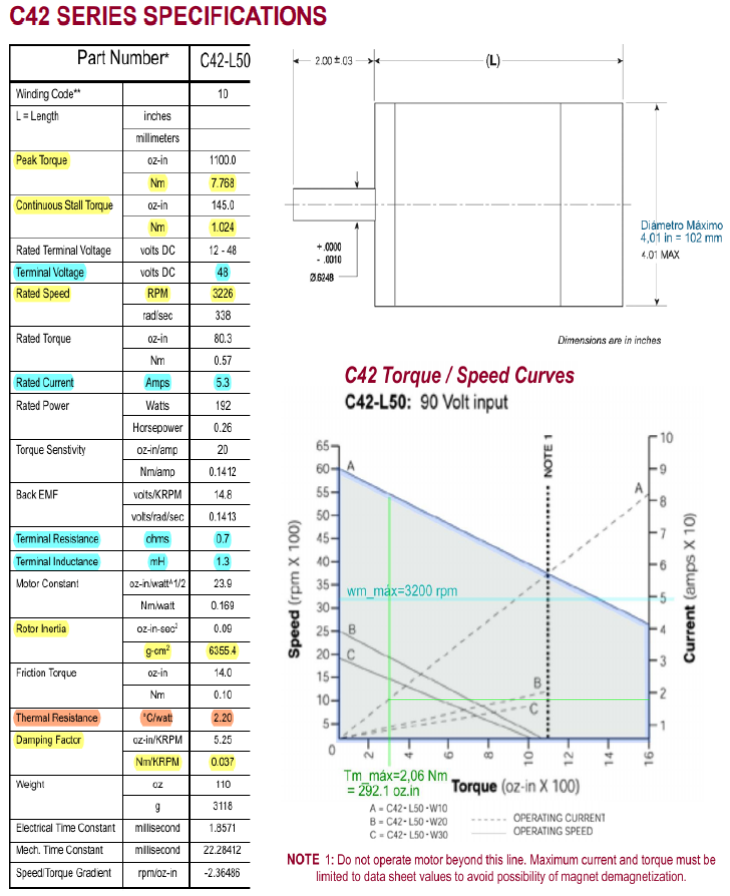
\includegraphics[width=0.9\textwidth]{Datos Datasheet Motor Brushed}
    \caption{Datos Datasheet Motor Brushed.}
    \label{fig:Datos Datasheet Motor Brushed}
\end{figure}




\subparagraph{Formulación del Modelo Mecánico Equivalente del Motor:}
\label{sec:Formulación del Modelo Mecánico Equivalente del Motor:}
\hfill

\hfill

El modelo equivalente del rotor del motor referido a su estator, el cual es un sistema inercial de referencia, está dado por:

\begin{subequations} \label{eq:J_m y theta_m}
    \begin{align}
        & \label{eq:J_m}   J_m.\ {\dot{\omega}}_m\left(t\right)=T_m\left(t\right)-b_m.\omega_m(t)-T_d(t)
        \\
        & \label{eq:theta_m}   {\dot{\theta}}_m\left(t\right)\equiv\omega_m\left(t\right)\ \ \Leftrightarrow{\ \ \theta}_m\left(t\right)=\int_{0}^{t}{\omega_m\left(\xi\right).d\xi}+\theta_m\left(0\right)
    \end{align}
\end{subequations}

Donde:
\begin{description}
    \item[$J_m:$] Momento de inercia del rotor junto con la caja reductora.
	\item[$b_m:$] Amortiguamiento viscoso del rotor junto con la caja reductora.
	\item[$\theta_m\left(t\right):$] Ángulo geométrico del motor.
	\item[$T_m\left(t\right):$] Torque electromagnético.
\end{description}

Parámetros mecánicos del motor y caja sumados:
\begin{subequations} \label{eq:J_m b_m}
    \begin{align}
        % & \label{eq:Valor de J_m}   J_m=3,1\times{10}^{-6}\ kg.m^2
        % \\
        % & \label{eq:Valor de b_m}   b_m=1,5\times{10}^{-5}\ \ \frac{N.m}{rad/s}
        & \label{eq:Valor de J_m}   J_m=6,356\times{10}^{-4}\ kg.m^2
        \\
        & \label{eq:Valor de b_m}   b_m=3,533\times{10}^{-4}\ \ \frac{N.m}{rad/s}
    \end{align}
\end{subequations}

\paragraph{SUBSISTEMA MECÁNICO COMPLETO}
\label{sec:SUBSISTEMA MECÁNICO COMPLETO}
\hfill

\hfill


A partir de los tres modelos mecánicos equivalentes obtenidos, se puede realizar una simplificación o compactación de los mismos para obtener un único modelo matemático equivalente del subsistema mecánico completo, el cual posee un solo grado de libertad.

\hfill

Subsistema Mecánico Completo = Carga Mecánica \ref{eq:J_l} + Caja Reductora \ref{eq:theta_l, omega_l y T_q} + Máquina Eléctrica \ref{eq:J_m}.

Despejando $T_q(t)$ de \ref{eq:J_l}:

\begin{align} \label{eq:SMC_7}
    T_q\left(t\right)=J_l.\ {\dot{\omega}}_l\left(t\right)+b_l.\omega_l(t)+T_l(t)
\end{align}

Remplazando $T_q(t)$ por \ref{eq:T_q}:

\begin{align} \label{eq:SMC_8-}
    r.T_d(t)=J_l.\ {\dot{\omega}}_l\left(t\right)+b_l.\omega_l(t)+T_l(t)
\end{align}

\begin{align} \label{eq:SMC_8}
    T_d(t)=\frac{J_l.\ {\dot{\omega}}_l\left(t\right)+b_l.\omega_l(t)+T_l(t)}{r}
\end{align}

Despejando $T_d(t)$ de \ref{eq:J_m}:

\begin{align} \label{eq:SMC_9}
    T_d(t)=T_m\left(t\right)-b_m.\omega_m(t)-J_m.\ {\dot{\omega}}_m\left(t\right)
\end{align}

Igualando $T_d(t)$ de \ref{eq:SMC_8} y \ref{eq:SMC_9}:

\begin{align} \label{eq:SMC_10-}
    T_m\left(t\right)-b_m.\omega_m(t)-J_m.\ {\dot{\omega}}_m\left(t\right)=\frac{J_l.\ {\dot{\omega}}_l\left(t\right)+b_l.\omega_l(t)+T_l(t)}{r}
\end{align}

\begin{align} \label{eq:SMC_10}
    J_m.\ {\dot{\omega}}_m\left(t\right)=T_m\left(t\right)-b_m.\omega_m(t)-\frac{J_l.\ {\dot{\omega}}_l\left(t\right)+b_l.\omega_l(t)+T_l(t)}{r}
\end{align}

Remplazando $\omega_l(t)$ por \ref{eq:omega_l}, y recordando que $\omega_m(t)={\dot{\theta}}_m(t)$, se puede escribir:

\begin{align} \label{eq:SMC_11-}
    J_m.\ {\dot{\omega}}_m\left(t\right)=T_m\left(t\right)-b_m.\omega_m(t)-\frac{J_l.\ \frac{{\dot{\omega}}_m\left(t\right)}{r}+b_l.\frac{\omega_m(t)}{r}+T_l(t)}{r}
\end{align}

\begin{align} \label{eq:SMC_11--}
    J_m.\ \ddot{\theta}_m\left(t\right)=T_m\left(t\right)-b_m.\dot{\theta}_m(t)-\ \frac{J_l}{r^2}.\ddot{\theta}_m\left(t\right)-\frac{b_l}{r^2}.\dot{\theta}_m(t)-\frac{T_l(t)}{r}
\end{align}

\begin{align} \label{eq:SMC_11}
    \left(J_m+\ \frac{J_l}{r^2}\right).\ {\ddot{\theta}}_m\left(t\right)=T_m\left(t\right)-\left(b_m+\frac{b_l}{r^2}\right).\dot{\theta}_m(t)-\frac{T_l(t)}{r}
\end{align}

En donde las expresiones obtenidas entre paréntesis son respectivamente el momento de inercia equivalente $J_{eq}(t)$ y el amortiguamiento viscoso equivalente $b_{eq}$ del subsistema mecánico completo:

\begin{subequations} \label{eq:J_eq y b_eq}
    \begin{align}
        & \label{eq:J_eq}   J_{eq}(t)=\left(J_m+\ \frac{J_l(t)}{r^2}\right)
        \\
        & \label{eq:b_eq}   b_{eq}=\left(b_m+\ \frac{b_l}{r^2}\right)
    \end{align}
\end{subequations}

% Jm = 6,356 × 10−4 ~[kg.m^2]
% J_{Z_{\text{mín.}}} =  0,56982 ~[kg.m^2]
% J_{Z_{\text{máx.}}} = 12,54696 ~[kg.m^2]
Sus valores son:
\begin{subequations} \label{eq:Valores de J_eq y b_eq}
	\begin{align}
        J_{eq_{\text{mín.}}}(t)=(J_m+\ \frac{J_{Z_{\text{mín.}}}}{r^2})= 6,58\times10^{-4} ~[kg.m^2]
        \\
        J_{eq_{\text{máx.}}}(t)=(J_m+\ \frac{J_{Z_{\text{máx.}}}}{r^2})= 1,126\times10^{-3} ~[kg.m^2]
        \\
        b_{eq}=(b_m+\ \frac{b_l}{r^2})=3,70\times10^{-4}\ \ \frac{N.m}{rad/s}
    \end{align}
\end{subequations}


Cabe notar que, como $J_l$ es un parámetro variable, entonces también lo es $J_{eq}$.

Así se escribe:

\begin{align} \label{eq:J}
    J_{eq}.\ \ddot{\theta}_m\left(t\right)={T_m\left(t\right)-b}_{eq}.\dot{\theta}_m(t)-\frac{T_l(t)}{r}
\end{align}

Además, también puede definir un torque de carga equivalente $T_{l_{eq}}(t)$ dado por:

\begin{align} \label{eq:T_l_eq}
    T_{l_{eq}}(t)=\frac{T_l(t)}{r}
\end{align}

\begin{align} \label{eq:J con T_l_eq}
    J_{eq}.\ \ddot{\theta}_m\left(t\right)={T_m\left(t\right)-b}_{eq}.\dot{\theta}_m(t)-T_{l_{eq}}(t)
\end{align}


Finalmente, se despeja la aceleración angular de \ref{eq:J}; y junto con \ref{eq:theta_m}, se obtienen las ecuaciones de estado que componen al modelo matemático equivalente del subsistema mecánico completo:

\begin{align} \label{eq:subsistema mecánico completo}
    \begin{cases}
        \dot{\theta}_m\left(t\right)=\omega_m\left(t\right)
        \\
        \dot{\omega}_m\left(t\right)=\frac{ -b_{eq}.\omega_m(t)+T_m\left(t\right)-\frac{T_l\left(t\right)}{r} }{ J_{eq}(t) }
    \end{cases}
\end{align}


En forma matricial:
\begin{align} \label{eq:subsistema mecánico completo en forma matricial}
    \begin{cases}
        \dot{x}\left(t\right)=\left[\begin{matrix}0&1\\0&-\frac{b_{eq}}{J_{eq}(t)}\\\end{matrix}\right]x\left(t\right)+\left[\begin{matrix}0&0\\\frac{1}{J_{eq}(t)}&-\frac{1}{{r.J}_{eq}(t)}\\\end{matrix}\right]u\left(t\right)
        \\
        y\left(t\right)=\left[\frac{1}{r}\ \ 0\right]x\left(t\right)
    \end{cases}
\end{align}

Donde:
\begin{description}
	\item[$x(t):$] Vector de estados.
	\item[$u(t):$] Vector de entradas.
	\item[$y(t):$] Vector de salidas.
\end{description}

\begin{align}  \label{eq:vectores de estados, entradas y salidas}
    x(t)=\left[\begin{matrix}\theta_m\left(t\right)\\\omega_m\left(t\right)\\\end{matrix}\right]
    &&
    u(t)=\left[\begin{matrix}T_m\left(t\right)\\T_l\left(t\right)\\\end{matrix}\right]
    &&
    y(t)=\theta_l\left(t\right)
\end{align}

En la figura \ref{fig:Diagrama de bloques del subsistema mecánico completo} se muestra el diagrama en bloques que representa al modelo del subsistema mecánico completo.

\begin{figure}[H]
    \centering
    \includegraphics[width=0.8\textwidth]{Diagrama de bloques del subsistema mecánico completo}
    \caption{Diagrama de bloques del subsistema mecánico completo.}
    \label{fig:Diagrama de bloques del subsistema mecánico completo}
\end{figure}


\subsubsection{SUBSISTEMA ELECTROMAGNÉTICO:}
\label{sec:SUBSISTEMA ELECTROMAGNÉTICO:}

El circuito equivalente de la armadura de un motor de CC, es mostrado en la figura \ref{fig:Circuito equivalente de la armadura de un motor de CC}. Dicho circuito se basa en el hecho de que el devanado de la armadura tiene una resistenci $R_a$, una auto-inductancia $L_a$, y una fuerza electromotriz (fem) inducida $e$.

\begin{figure}[H]
    \centering
    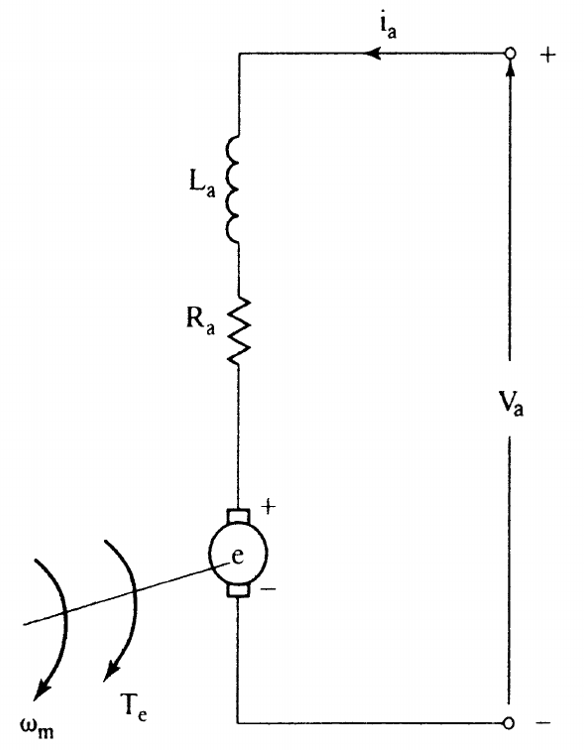
\includegraphics[width=0.4\textwidth]{Circuito equivalente de la armadura de un motor de CC}
    \caption{Circuito equivalente de la armadura de un motor de CC.}
    \label{fig:Circuito equivalente de la armadura de un motor de CC}
\end{figure}

Donde:
\begin{description}
	\item[$v_a:$] Voltaje (externo) de armadura.
    \item[$i_a:$] Corriente de armadura.
    \item[$R_a:$] Resistencia de armadura.
    \item[$L_a:$] Inductancia de armadura.
    \item[$e:$]  Fem inducida (en la armadura).
\end{description}

Para una máquina de CC con P polos y Z conductores en su armadura, con un flujo de campo por polo $\phi_f$ y con una velocidad de rotación de $n_r$ rpm, la expresión de la fem inducida se deduce de la ley de Faraday, sin tener en cuenta el signo, como:

\begin{align}   \label{eq:e1}
    e=Z.\frac{d\phi_f}{dt}=Z.\frac{\phi_f}{t}
\end{align}

En donde t es el tiempo en el que los conductores cortan $\phi_f$ líneas de flujo:

\begin{align}   \label{eq:e2}
    t=\frac{1}{2xfrecuencia}=\frac{1}{2.\frac{P}{2}.\frac{n_r}{60}}
\end{align}

El flujo ocurre para cada par de polos. Sustituyendo \ref{eq:e2} en \ref{eq:e1}:

\begin{align}   \label{eq:e3}
    e=\frac{Z.\phi_f.P.n_r}{60}
\end{align}

Si los conductores de la armadura se dividen en '$a$' caminos paralelos, entonces:

\begin{align}   \label{eq:e4}
    e=\frac{Z.\phi_f.P.n_r}{60.a}
\end{align}

Hay dos arreglos posibles de los conductores de la armadura, los devanados en serie y los devanados en paralelo. Los valores para '$a$' en cada caso son:

\begin{align} \label{eq:e5}
    a=
    \begin{cases}
        2\ \text{para devanado en serie}
        \\
        P\ \text{para devanado en paralelo}
    \end{cases}
\end{align}

Es usual escribir la ecuación \ref{eq:e4} de una forma más compacta como:

\begin{align}   \label{eq:e6}
    e=K.\phi_f.\omega_m
\end{align}

Donde $\omega_m=\frac{2.\pi.n_r}{60}\ \frac{rad}{s}$ y $K=(\frac{P}{a}).Z.(\frac{1}{2.\pi})$

\hfill


Y si el flujo de campo es constante en la máquina de CC, entonces su fem inducida es proporcional a la velocidad de su rotor.
Este es el caso en los motores (con escobillas de CC) con excitación separada pero con corriente de campo constante; y también es el caso en los motores con imanes permanentes, debido claramente a que el campo magnético se genera por los imanes permanentes.

\begin{align}   \label{eq:e expresada en función de K_E}
    e=K_E.\omega_m
\end{align}

Donde:
\begin{description}
	\item[$K_E:$] Constante de la fem inducida.
\end{description}

\begin{align}   \label{eq:K_E}
    K_E=K.\phi_f\ \frac{V}{\frac{rad}{s}}
\end{align}


Retomando el circuito equivalente de la armadura de un motor de CC \ref{fig:Circuito equivalente de la armadura de un motor de CC}, al aplicar la Ley de Kirchhoff de las espiras sobre dicho circuito, la cual se basa en el balance de las diferencias de potencial eléctrico, se obtiene la ecuación:

\begin{align}   \label{eq:v_a}
    v_a=R_a.i_a+L_a.\frac{di_a}{dt}+e
\end{align}

Siendo para el motor seleccionado \cite{MoogMotorDatasheet}:
\begin{subequations} \label{eq:R_a L_a v}
    \begin{align}
        % & \label{eq:Valor de v_a}   v_a=48\ V
        % \\
        & \label{eq:Valor de R_a}   R_a=0,7\ ohm
        \\
        & \label{eq:Valor de L_a}   L_a=1,3\ mH
    \end{align}
\end{subequations}

En estado estacionario, la $i_a$ es constante, de esta forma la equación del voltaje de armadura se reduce a:

\begin{align}   \label{eq:v_a reducida}
    v_a=R_a.i_a+e
\end{align}

El balance de potencia se obtiene al multiplicar ambos miembros por $i_a$:

\begin{align}   \label{eq:v_a.i_a}
    v_a.i_a=R_a.i_a^2+e.i_a
\end{align}

El términio $v_a.i_a$ es la potencia total suministrada al motor, y el término $R_a.i_a^2$ representa las pérdidas por efecto Joule en el cobre. Por lo tanto, $e.i_a$ denota la potencia efectiva que se transforma de eléctrica a mecánica, la cual se la puede expresar en términos del torque electromagnético y de la velocidad como:

\begin{align}   \label{eq:P_a}
    P_a=e.i_a=\omega_m.T_m
\end{align}

Donde:
\begin{description}
	\item[$P_a:$] Potencia efectiva.
\end{description}

Despejando el torque electromagnético:

\begin{align}   \label{eq:T_m}
    T_m=\frac{e.i_a}{\omega_m}
\end{align}

Reemplazando \ref{eq:e expresada en función de K_E} en \ref{eq:T_m}, pero remplazando $K_E$ por $K_T$,se obtiene una representación más simple del torque electromagnético como:

\begin{align}   \label{eq:T_m expresada en función de K_T}
    T_m=K_T.i_a
\end{align}

Siendo para el motor seleccionado \cite{MoogMotorDatasheet}:
\begin{align}   \label{eq:Valor de K_T}
    K_T=0,1412\ \frac{N.m}{A}
\end{align}

Donde $K_E=K_T$ siempre que el flujo de campo permanezca constante (como es el caso), y siempre que obviamente dichas constantes y todos los parámetros se expresen en el mismo sistema de unidades (sistema internacional de unidades).

En resumen, el subsistema electromagnético se encuentra dado por la ecuación \ref{eq:v_a}, la cual al despejar la derivada en el tiempo de la variable de estado $i_a$, se obtiene la ecuación de estado del subsistema electromagnético \ref{eq:subsistema electromagnético}.

\begin{align}   \label{eq:subsistema electromagnético}
    \frac{di_a}{dt}=\frac{v_a-R_a.i_a-e}{L_a}
\end{align}



\begin{figure}[H]
    \centering
    \includegraphics[width=0.7\textwidth]{Diagrama de bloques del subsistema electromagnético}
    \caption{Diagrama de bloques del subsistema electromagnético.}
    \label{fig:Diagrama de bloques del subsistema electromagnético}
\end{figure}

Mientras que las ecuaciones \ref{eq:e expresada en función de K_E} y \ref{eq:T_m expresada en función de K_T} sirven para realacionar a los subsistemas mecánico y electromagnético, debido a que representan la conversión de energía electromecánica en ambos sentidos.


\begin{figure}[H]
    \centering
    \includegraphics[width=0.3\textwidth]{Diagramas de bloques de los conversores electromecánicos}
    \caption{Diagramas de bloques de los conversores electromecánicos.}
    \label{fig:Diagramas de bloques de los conversores electromecánicos}
\end{figure}

% \subsubsection{SUBSISTEMA TÉRMICO:}
% \label{sec:SUBSISTEMA TÉRMICO:}

\subsubsection{MODELO COMPLETO DE LA PLANTA:}
\label{sec:MODELO COMPLETO DE LA PLANTA:}

Una vez descritas las ecuaciones (diferenciales de primer orden) que modelan a cada subsistema, es posible reorganizarlas y combinarlas de tal forma de representar al sistema físico completo como un conjunto de variables de entrada, de salida y de estado.

Reemplazando $T_m$ de la ecuación \ref{eq:subsistema mecánico completo} del subsistema mecánico por la expresión \ref{eq:T_m expresada en función de K_T}, y reemplazando $e$ de la ecuación \ref{eq:subsistema electromagnético} del subsistema electromagnético por la expresión \ref{eq:e expresada en función de K_E}, se obtiene el modelo en espacio de estados del sistema completo:

\begin{align} \label{eq:modelo completo de la planta}
    \begin{cases}
        \dot{\theta}_m\left(t\right)=\omega_m\left(t\right)
        \\
        \dot{\omega}_m\left(t\right)=\frac{ -b_{eq}.\omega_m(t)+K_T.i_a(t)-\frac{T_l\left(t\right)}{r} }{ J_{eq}(t) }
        \\
        \frac{di_a}{dt}=\frac{v_a(t)-R_a.i_a(t)-K_E.\omega_m(t)}{L_a}
    \end{cases}
\end{align}

Siendo la ecuación de salida:
\begin{align} \label{eq:ecuación de salida}
    y(t) = \theta_l(t)
\end{align}

En forma matricial:
\begin{align} \label{eq:modelo completo de la planta en forma matricial}
    \begin{cases}
        \dot{x}\left(t\right)=\left[\begin{matrix}0&1&0\\0&-\frac{b_{eq}}{J_{eq}(t)}&\frac{K_T}{J_{eq}(t)}\\0&\frac{-K_E}{L_a}&-\frac{R_a}{L_a}\\\end{matrix}\right]x\left(t\right)+\left[\begin{matrix}0&0\\0&-\frac{1}{{r.J}_{eq}(t)}\\\frac{1}{L_a}&0\\\end{matrix}\right]u\left(t\right)
        \\
        y\left(t\right)=\left[\frac{1}{r}\ \ 0\ \ 0\right]x\left(t\right)+\left[0\ \ 0\ \ 0\right]u\left(t\right)
    \end{cases}
\end{align}

Donde:
\begin{description}
	\item[$x(t):$] Vector de estados.
	\item[$u(t):$] Vector de entradas.
	\item[$y(t):$] Vector de salidas.
\end{description}

\begin{align}  \label{eq:vectores de estados, entradas y salidas de la planta completa}
    x(t)=\left[\begin{matrix}\theta_m\left(t\right)\\\omega_m\left(t\right)\\i_a\left(t\right)\\\end{matrix}\right]
    &&
    u(t)=\left[\begin{matrix}v_a\left(t\right)\\T_l\left(t\right)\\\end{matrix}\right]
    &&
    y(t)=\theta_l\left(t\right)
\end{align}

Se observa en las ecuaciones escalares, que se trata de un sistema de tercer orden, ya que posee tres variables de estado. Cada variable de estado corresponde a un elemento almacenador de energía que compone al sistema:
\begin{itemize}
    \item [$\theta_m(t):$] Al considerar un acoplamiento rígido entre motor y la carga mecánica, entonces la variable de estado $\theta_m\left(t\right)$ no se relaciona con un almacenamiento real de energía elástica, aunque si es una variable de estado, siendo una excepción a la correspondencia con el almacenamiento de energía.
    \item [$\omega_m(t):$] Los momentos de inercia sumados, del rotor del motor, del reductor armónico, y de la articulación base del robot, almacenan energía cinética, energía que depende de $\omega_m(t):$ (o bien de $\omega_l(t):$), la cual es una de las variables de estado del modelo global.
    \item [$i_a(t):$] Los bobinados de la armadura son inductores que almacenan energía electromagnética, por lo que la corriente de armadura $i_a(t)$ es otra variable de estado del sistema.
\end{itemize}
En donde, el vector de entradas $u(t)$ se conforma de una entrada que se puede manipular $(v_a)$ y otra entrada que representa las perturbaciones $(T_L)$.


De esta forma, quedan definidas las matrices A,B,C y D del modelo del sistema \ref{eq:modelo completo de la planta en forma matricial}, el cual se da en concordancia con un sistema matricial lineal de parámetros variables (LPV), con el único parámetro variable $J_{eq}(t)$:

\begin{align} \label{eq:sistema lineal de parámetros variables en el tiempo LPV}
    \begin{cases}
        \dot{x}\left(t\right)=A(J_{eq}).x(t)+B(J_{eq}).u(t)
        \\
        y\left(t\right)=C.x(t)+D.u(t)
    \end{cases}
\end{align}

Donde $J_{eq}=J_{eq}(t)$ es función de las posiciones articulares del robot.

A continuación se muestra el diagrama en bloques que representa al modelo completo de la planta:

\begin{figure}[H]
    \centering
    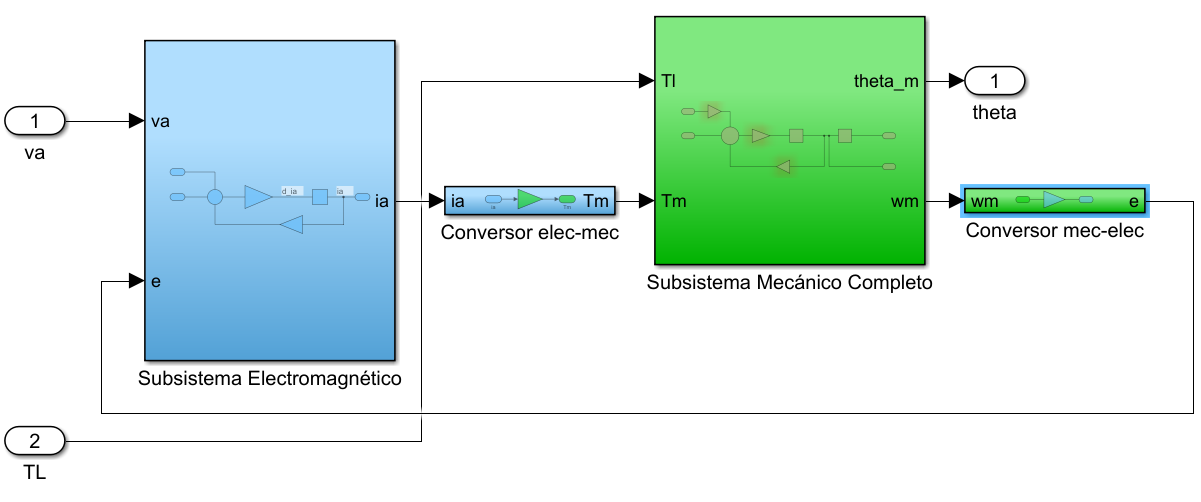
\includegraphics[width=1\textwidth] {Diagrama en bloques de la Planta}
    \caption{Diagrama en bloques de la Planta.}
    \label{fig:Diagrama en bloques de la Planta}
\end{figure}


\subsection{ANÁLISIS DEL MODELO DE LA PLANTA}
\label{sec:ANÁLISIS DEL MODELO DE LA PLANTA}

Antes de realizar el diseño del controlador, y la validación del modelo completo de la planta, se procede a verificar dicho modelo matemático, analizando su estabilidad, controlabilidad y observabilidad.

\subsubsection{ESTABILIDAD Y AMORTIGUAMIENTO DE LA PLANTA}
\label{sec:ESTABILIDAD Y AMORTIGUAMIENTO DE LA PLANTA}

\paragraph{Criterio De Estabilidad:}
\label{sec:Criterio De Estabilidad:}
\hfill

\hfill

La estabilidad de la planta puede ser determinada a través de sus polos. El criterio de estabilidad dice que el sistema es estable si todos los polos del sistema poseen parte real negativa, ya que corresponden a realimentaciones negativas. En cambio, si tal solo hubiera un polo con parte real positiva se tendría una realimentación positiva que llevaría a una divergencia en la salida, es decir, el sistema sería inestable.

Los polos del sistema son los autovalores de la matriz A del sistema, por lo que se los puede obtener al calcular dichos autovalores.
Otra forma de obtenerlos es a partir de las funciones de transferencia en el dominio complejo para cada entrada, donde las raíces del polinomio del denominador de dichas funciones de transferencia, son los polos del sistema.
Sin embargo, existe otra manera más sencilla para evaluar la estabilidad del sistema, la cual es el Criterio de Estabilidad de Routh que se cita a continuación:

\hfill

\textbf{Criterio de estabilidad de Routh:} Para un polinomio en S con coeficientes $a_n$ reales, si cualquiera de los coeficientes es negativo o nulo (luego de haber removido las raíces nulas) en presencia de al menos un coeficiente positivo, entonces existen raíces con parte real positiva, lo que implica inestabilidad en el sistema.

Para obtener las funciones de transferencia del sistema, se retoman la segunda y tercer ecuación de estado de la planta \ref{eq:modelo completo de la planta}:

\begin{align} \label{eq:Funciones de Transferencia 1}
    \dot{\omega}_m\left(t\right)=\frac{ -b_{eq}.\omega_m(t)+K_T.i_a(t)-\frac{T_l\left(t\right)}{r} }{ J_{eq}(t) }
    \\
    \frac{di_a}{dt}=\frac{v_a(t)-R_a.i_a(t)-K_E.\omega_m(t)}{L_a}
\end{align}

Y se les aplica la transformada de Laplace para pasarlas del dominio del tiempo al dominio de la frecuencia:

\begin{align}
    & \label{eq:Funciones de Transferencia 2a} \theta_m\left(S\right).S^2=\frac{-b_{eq}{.\theta}_m\left(S\right).S+K_T.i_a\left(S\right)-\frac{T_l\left(S\right)}{r}}{J_{eq}}
    \\
    & \label{eq:Funciones de Transferencia 2b} i_a(S).S=\frac{v_a\left(S\right)-R_a.i_a\left(S\right)-K_E.\theta_m\left(S\right).S}{L_a}
\end{align}

Despejando $i_a(S)$ de \ref{eq:Funciones de Transferencia 2b}, y reemplazándola en \ref{eq:Funciones de Transferencia 2a}, se obtiene:

\begin{align} \label{eq:Funciones de Transferencia 3}
    {J_{eq}.\theta}_m\left(S\right).S^2=-b_{eq}{.\theta}_m\left(S\right).S+K_T.\left(\frac{v_a\left(S\right)-K_E.\theta_m\left(S\right).S}{L_a.S+R_a}\right)-\frac{T_l\left(S\right)}{r}
\end{align}

\begin{align} \label{eq:Funciones de Transferencia 4}
    \left[J_{eq}.S^2+\left(b_{eq}+\frac{K_T.K_E}{L_a.S+R_a}\right).S\right].\theta_m\left(S\right)=\frac{K_T}{L_a.S+R_a}.v_a\left(S\right)-\frac{T_l\left(S\right)}{r}
\end{align}

Para obtener la función de transferencia respecto a la entrada $v_a(t)$, en \ref{eq:Funciones de Transferencia 4} se toma a $T_l(t)=0$, y se despeja el cociente de la salida sobre dicha entrada:

\begin{align} \label{eq:Funciones de Transferencia 5}
    \frac{\theta_m\left(S\right)}{v_a\left(S\right)}=\frac{\frac{K_T}{L_a.S+R_a}}{J_{eq}.S^2+\left(b_{eq}+\frac{K_T.K_E}{L_a.S+R_a}\right).S}
\end{align}

\begin{align} \label{eq:Funciones de Transferencia 6}
    \frac{\theta_m\left(S\right)}{v_a\left(S\right)}=\frac{K_T}{\left(L_a.S+R_a\right).\left[J_{eq}.S^2+\left(b_{eq}+\frac{K_T.K_E}{L_a.S+R_a}\right).S\right]}
\end{align}

\begin{align} \label{eq:Funciones de Transferencia 7}
    \frac{\theta_m\left(S\right)}{v_a\left(S\right)}=\frac{K_T}{{(L_a.J}_{eq}).S^3+{(R_a.J}_{eq}+L_a.b_{eq}).S^2+\left(R_a.b_{eq}+K_T.K_E\right).S}
\end{align}

\textbf{\begin{align} \label{eq:Funciones de Transferencia G_va(S)}
    G_{v_a}\left(S\right)=\frac{\theta_m\left(S\right)}{v_a\left(S\right)}=\frac{K_T}{S.\left[{(L_a.J}_{eq}).S^2+{(R_a.J}_{eq}+L_a.b_{eq}).S+\left(R_a.b_{eq}+K_T.K_E\right)\right]}
\end{align}}

Y para obtener la función de transferencia respecto a la entrada $T_l(t)$, en \ref{eq:Funciones de Transferencia 4} se toma a $v_a(t)=0$, y se despeja el cociente de la salida sobre dicha entrada:


\begin{align} \label{eq:Funciones de Transferencia 9}
    \frac{\theta_m\left(S\right)}{T_l\left(S\right)/r}=\frac{-\left(L_a.S+R_a\right)}{\left(L_a.S+R_a\right).\left[J_{eq}.S^2+\left(b_{eq}+\frac{K_T.K_E}{L_a.S+R_a}\right).S\right]}
\end{align}


\begin{align} \label{eq:Funciones de Transferencia 10}
    \frac{\theta_m\left(S\right)}{T_l\left(S\right)/r}=\frac{\theta_m\left(S\right)}{T_{eq}\left(S\right)}=\frac{-L_a.S-R_a}{\left({L_a.J}_{eq}\right).S^3+\left(R_a.J_{eq}+L_a.b_{eq}\right).S^2+\left(R_a.b_{eq}+K_T.K_E\right).S}
\end{align}


\textbf{\begin{align} \label{eq:Funciones de Transferencia G_Teq(S)}
    G_{T_{eq}}\left(S\right)=\frac{\theta_m\left(S\right)}{T_l\left(S\right)/r}=\frac{\theta_m\left(S\right)}{T_{eq}\left(S\right)}=\frac{-L_a.S-R_a}{S.\left[\left({L_a.J}_{eq}\right).S^2+\left(R_a.J_{eq}+L_a.b_{eq}\right).S+\left(R_a.b_{eq}+K_T.K_E\right)\right]}
\end{align}}

Se observa que se tiene la ecuación característica: $S.[({L_a.J}_{eq}).S^2+(R_a.J_{eq}+L_a.b_{eq}).S+(R_a.b_{eq}+K_T.K_E)]$, la cual posee todos sus coeficientes positivos, ya que están conformados por variables escalares que físicamente solo pueden tener un valor positivo. Por lo tanto el Criterio de estabilidad de Routh no dice que el sistema es estable. Aunque debido a que se tiene un polo en cero, la planta es marginalmente estable, es decir se encuentra al límite entre ser estable o inestable. Pero, para resolver esto, se implementará un controlador, de tal forma que este cambie el comportamiento del sistema, reubicando los polos para obtener un sistema controlador-planta más estable y por lo tanto más robusto.


\paragraph{Parámetros De Segundo Orden de la Planta:}
\label{sec:Parámetros De Segundo Orden de la Planta:}
\hfill

\hfill

Por otra parte, a partir del polinomio característico, es posible encontrar los dos parámetros del sistema de segundo orden, que son la frecuencia angular natural $\omega_n$, y el factor de amortiguamiento $\zeta$. Los cuales aportan información relevante para la convergencia y la estabilidad de la respuesta del sistema.

Para ello se parte se parte de la expresión de un sistema de segundo orden:

\begin{align} \label{eq:Expresión del Polinomio Característico}
    P\left(s\right)=S.\left[S^2+\left(2.\zeta.\omega_n\right).S+\omega_n^2\right]
\end{align}

Se toma al polinomio característico del sistema, y se dividen todos sus términos por su coeficiente principal, obteniendo:

\begin{align} \label{eq:Polinomio Característico del Sistema}
    P\left(s\right)=S.\left[S^2+\left(\frac{R_a.J_{eq}+L_a.b_{eq}}{L_a.J_{eq}}\right).S+\left(\frac{R_a.b_{eq}+K_T.K_E}{L_a.J_{eq}}\right)\right]
\end{align}

Entonces se pueden igualar los términos de ambas expresiones, de donde se obtienen las expresiones para $\omega_n$ y $\zeta$:

\begin{align} \label{eq:Frecuencia Natural}
    \omega_n=\sqrt{\frac{R_a.b_{eq}+K_T.K_E}{L_a.J_{eq}}}
\end{align}

\begin{align} \label{eq:Factor de Amortiguamiento}
    \zeta=\frac{R_a.J_{eq}+L_a.b_{eq}}{L_a.J_{eq}\text{.2}.\omega_n}
\end{align}

Particularmente, al tratarse de un sistema LPV, el análisis del modelo debe realizarse para varios valores del parámetro variable $J_{eq}(t)$, para así tener una mayor certeza de que el sistema se comporte como se espera, en todos sus puntos de operación. Entonces se procede a tomar 4 valores de $J_l(t)$, igualmente separados por un paso igual a:

\begin{align} \label{eq:Paso para la selección de los valores del parámetro variable J_l(t)}
    \frac{J_{l_{\text{máx.}}}-J_{l_{\text{mín.}}}}{4}=3,99238 ~[kg.m^2]
\end{align}

Paso con el que se obtienen los siguientes 4 valores para $J_l$:

\begin{align} \label{eq:Valores elegidos de Jl}
    J_l=\left[0,57\ ;\ 4,56\ ;\ 8,55\ ;\ 12,5\right] ~[kg.m^2]
\end{align}

Y utilizando la ecuación \ref{eq:J_eq}, se obtienen los correspondientes 4 valores para $J_{eq}(t)$:

\begin{align} \label{eq:Valores correspondientes de Jeq}
    J_{eq}=\left[6,58\times{10}^{-4};8,14\times{10}^{-4};9,78\times{10}^{-4};11,3\times{10}^{-4}\right] ~[kg.m^2]
\end{align}

En la tabla \ref{table:Valores de omega_n y zeta, eligiendo 4 valores para Jl}, se muestran los valores de $\omega_n$ y $\zeta$ para los distintos valores elegidos del parámetro variable $J_l(t)$.

\begin{table}[H]
    \centering
    \begin{tabular}{|l|llll|}
    \cline{1-5}
    \textbf{$J_l ~[kg.m^2]$}     &   0,57  &   4,56   &   8,55   &  12,5    \\ \cline{1-5}
    \textbf{$\omega_n ~[rad/s]$} & 153,657 & 138,1508 & 126,5552 & 117,4618 \\ \cline{1-5}
    \textbf{$\zeta$}             &   1,754 &   1,9505 &   2,1289 &   2,2935 \\ \cline{1-5}
    \end{tabular}
    \caption{\label{table:Valores de omega_n y zeta, eligiendo 4 valores para Jl}Valores de $\omega_n$ y $\zeta$, eligiendo 4 valores para $J_l$.}
\end{table}

Como se observa, el factor de amortiguamiento es siempre mayor a la unidad, lo que significa que el sistema es sobreamortiguado. Esto se cumple para todos los valores de $J_l$ considerados.


\paragraph{Mapa De Polos Y Ceros de la Planta:}
\label{sec:Mapa De Polos Y Ceros de la Planta:}
\hfill

\hfill

Mediante la función: solve(eqn,var) de MATLAB, se calcula la variable S para el polinomio característico igualado a cero. Es decir, se calculan sus raíces, con lo que se obtienen los polos del sistema, los cuales se muestran en la siguiente tabla:

\begin{table}[H]
    \centering
    \begin{tabular}{|l|llll|}
    \cline{1-5}
    \textbf{$J_l ~[kg.m^2]$}    &    0,57 &    4,56 &    8,55  &   12,5  \\ \cline{1-5}
    \textbf{$S_1$}              &    0    &    0    &    0     &    0    \\ \cline{1-5}
    \textbf{$S_2$}              & -490,9  & -500,8  & -507,3   & -511,8  \\ \cline{1-5}
    \textbf{$S_3$}              &  -48,1  &  -38,1  &  -31,6   &  -27,0  \\ \cline{1-5}
    \end{tabular}
    \caption{\label{table:Polos del sistema para los 4 valores de Jl elegidos}Polos del sistema para los 4 valores de $J_l$ elegidos.}
\end{table}

En donde, al no haber ningún polo positivo, se corrobora que se trata de un sistema estable.

Luego, utilizando la función de MATLAB: pzmap(sys), se gráfican los polos y ceros de la planta en el plano complejo, de su función de tranfrerencia respecto a la entrada manipulada $v_a$, para cada uno de los valores de $J_l$ elegidos, como se muestra a continuación:

\begin{figure}[H]
    \centering
    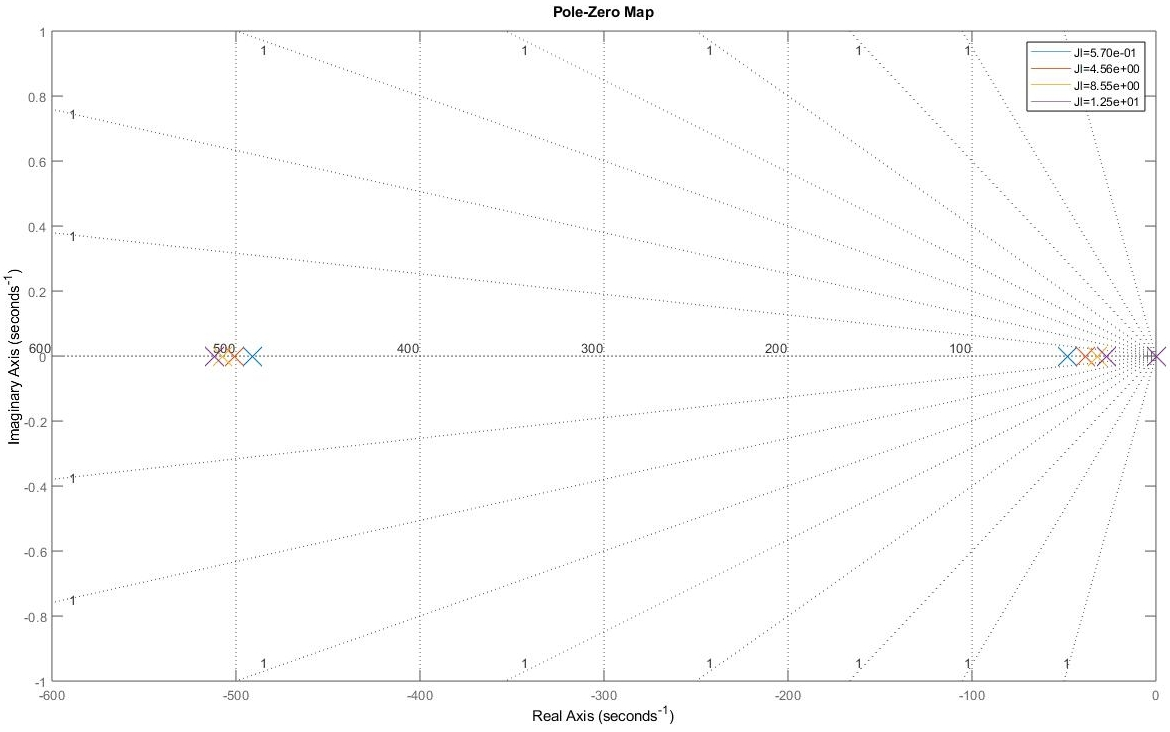
\includegraphics[width=1\textwidth]{Polos y Ceros de la Planta, respecto a la Entrada Manipulada}
    \caption{Polos y Ceros de la Planta, respecto a la Entrada Manipulada.}
    \label{fig:Polos y Ceros de la Planta, respecto a la Entrada Manipulada}
\end{figure}

En donde, se observa la ausencia de ceros de la planta al tratarse de un polinomio de grado cero en el numerador de su función de transferencia $G_{v_a}$. Además, se observa que todos los polos no poseen parte imaginaria, lo que corrobora que el sistema no oscila.

\paragraph{Diagrama De Bode de la Planta:}
\label{sec:Diagrama De Bode de la Planta:}
\hfill

\hfill

Además, utilizando la función de MATLAB: bode(sys), se gráfican los diagramas de Bode, de la función de transferencia de la planta respecto a la entrada manipulada $v_a$, para cada uno de los valores de $J_l$ elegidos, como se muestra a continuación:

\begin{figure}[H]
    \centering
    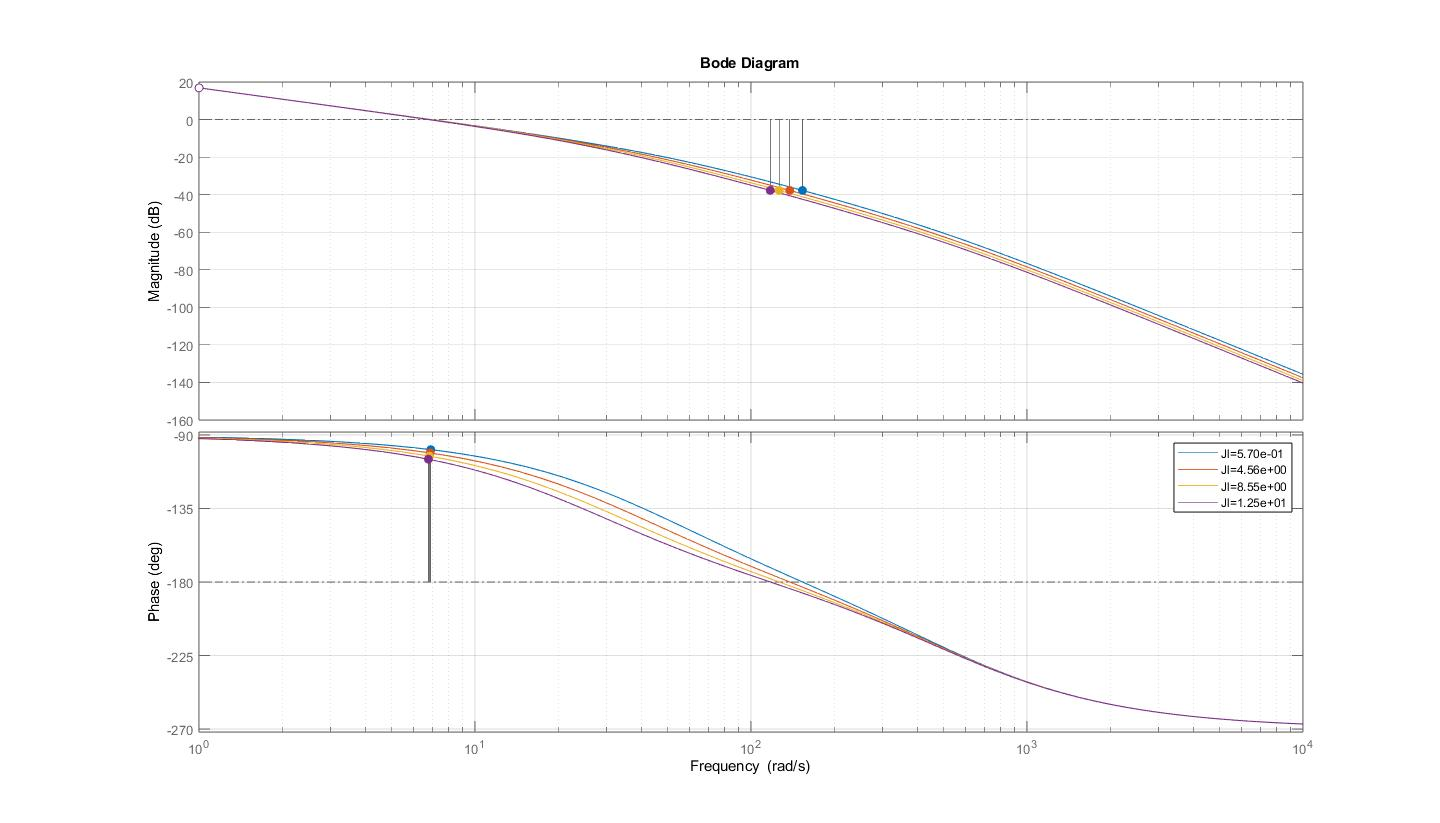
\includegraphics[width=1\textwidth]{Diagrama de Bode de la Planta, respecto a la Entrada Manipulada}
    \caption{Diagrama de Bode de la Planta, respecto a la Entrada Manipulada.}
    \label{fig:Diagrama de Bode de la Planta, respecto a la Entrada Manipulada}
\end{figure}

En donde se observa los valores de \textbf{Margen de ganancia Mg} y \textbf{Margen de fase Mf} posee la planta. Los cuales dicen respectivamente cuanto aumento solo en la ganancia, y cuanto aumento solo en la fase, puede absorber el sistema sin volverse inestable. Y al ser relativamente grandes dichos valores obtenidos, se puede decir, aunque sin asegurarlo, que es sistema es lo suficientemente robusto.

Y para asegurar que la planta es realmente robusta, se obtiene el valor de su \textbf{sensibilidad Ms}. La sensivilidad dice cómo las variaciones en los parámetros de la planta, afectan a su función de transferencia en lazo cerrado (con realimentación unitaria). En general, se busca que la sensibilidad sea lo suficientemente alta (típicamente $Ms>0,01$) para detectar cambios significativos en la entrada y generar una respuesta adecuada, pero no tan alta (típicamente $Ms<1,3$ o $Ms<2$) como para generar fácilmente inestabilidades en el sistema. A continuación, se muestra el diagrama de Bode de la sensibilidad a lazo cerrado con realimentación unitaria para los distintos valores de $J_l$:

\begin{figure}[H]
    \centering
    \includegraphics[width=1\textwidth]{Diagrama de Bode de la Sensibilidad a lazo cerrado con realimentación unitaria}
    \caption{Diagrama de Bode de la Sensibilidad a lazo cerrado con realimentación unitaria.}
    \label{fig:Diagrama de Bode de la Sensibilidad a lazo cerrado con realimentación unitaria}
\end{figure}

De donde se puede obserbar un valor pico en la magnitud de la sensibilidad de 1,09 dB para $J_l=12,5 ~[kg.m^2]$ y de 0,922 dB para $J_l=0,57 ~[kg.m^2]$. Valores que al convertirlos desde los decibeles, dan lugar a los valores de sensibilidad:

\begin{subequations} \label{eq:Valores de Sensibilidad}
	\begin{align}
        Ms=10^{\frac{1,09 ~\text{dB}}{20}}=1,13 ~~~(\text{para:}~ J_l=12,5 ~[kg.m^2])
        \\
        Ms=10^{\frac{0,922 ~\text{dB}}{20}}=1,11 ~~~(\text{para:}~ J_l=0,57 ~[kg.m^2])
	\end{align}
\end{subequations}

Valores que se encuentran dentro de los valores de sensibilidad típicos, lo que confirma que la planta es robusta.


\subsubsection{RESPUESTA DE LA PLANTA A LAZO ABIERTO}
\label{sec:RESPUESTA DE LA PLANTA A LAZO ABIERTO}

A continuación, utilizando Simulink se obtiene la respuesta en la posición $\theta_l$, velocidad $\omega_l$ y corriente $i_a$ de la planta, ante una entrada escalón de $v_a=48$ V aplicada a los 0,1 s, y una entrada escalón de $T_l=330$ N.m aplicada a los 0,5 s.

\begin{figure}[H]
    \centering
    \includegraphics[width=1\textwidth]{Consignas escalón de va y Tl}
    \caption{Consignas escalón de va y Tl.}
    \label{fig:Consignas escalón de va y Tl}
\end{figure}

\begin{figure}[H]
    \centering
    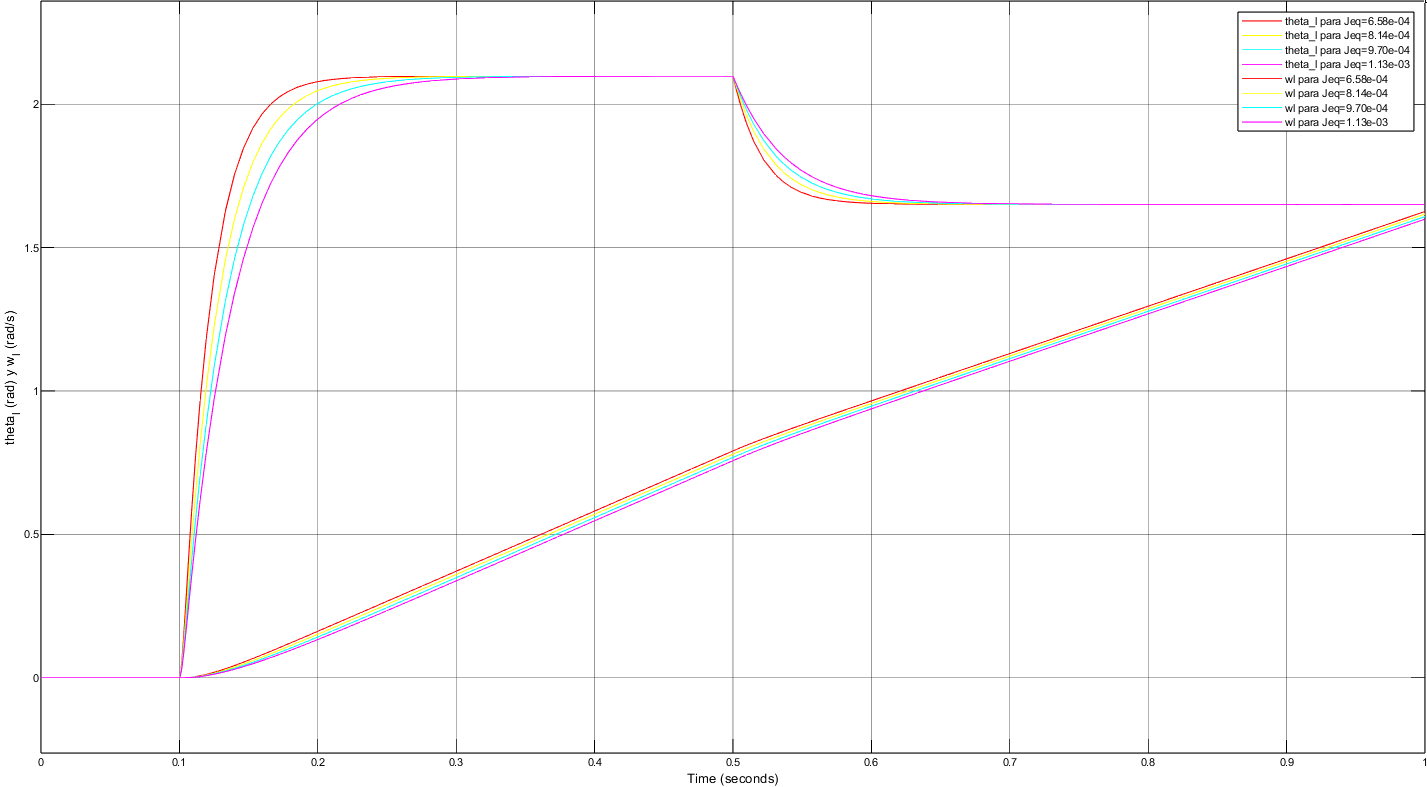
\includegraphics[width=1\textwidth]{Respuesta en la posición y velocidad de la planta ante un escalón de va y de Tl}
    \caption{Respuesta en la posición y velocidad de la planta ante un escalón de va y de Tl.}
    \label{fig:Respuesta en la posición y velocidad de la planta ante un escalón de va y de Tl}
\end{figure}

\begin{figure}[H]
    \centering
    \includegraphics[width=1\textwidth]{Respuesta en la corriente armadura de la planta ante un escalón de va y de Tl}
    \caption{Respuesta en la corriente armadura de la planta ante un escalón de va y de Tl.}
    \label{fig:Respuesta en la corriente armadura de la planta ante un escalón de va y de Tl}
\end{figure}

Las gráficas dejan en evidencia que el sistema no oscila en su respuesta a las variaciones repentinas de las entradas.
En el caso de la corriente, en \ref{fig:Respuesta en la corriente armadura de la planta ante un escalón de va y de Tl} se observa un pico de unos 60 A (61,3 A para el peor caso correspondiente al $J_{l_{\text{máx.}}})$), y también se observa una corriente constante ante la respuesta escalón a la máxima carga $T_l$, igual a 15,4 A, cuando la corriente nominal del motor es de solo 5,3 A.
% Por otro lado, se observa que la perturbación obviamente cambia el valor final de la posición angular, y lo hace en 25°.
% De esta forma se concluye que el sistema a lazo abierto requiere de una metodología de control, para mantener el valor de la variable interna $i_a(t)$ dentro de los rangos de seguridad del dispositivo.

\subsubsection{VALIDACIÓN DE LA PLANTA}
\label{sec:VALIDACIÓN DE LA PLANTA}

La validación es el proceso de determinar el grado de precisión con el que el modelo representa al mundo real, desde la perspectiva de los usos previstos del modelo.

Se procede validar el sistema desarrollado. A falta de disponer físicamente del robot, la validación del modelo propuesto de la planta a controlar se realizaría comparándolo con un modelo matemático más cercano a la realidad, elaborado teniendo en cuenta las no linealidades del robot.

Se tiene que el \textbf{modelo de diseño (de la planta)} obtenido, es ul conjunto de modelos lineales que se obtienen para distintos valores a elección del parámetro variable $J_l=J_Z$.

Y se tiene que el \textbf{modelo de validación (de la planta)}, sería un único modelo que incluiría todas las no linealidades del robot. Pero en realidad este modelo no lineal terminaría siendo lo mismo que el modelo lineal, porque:

\textbf{1) No se necesita considerar el modelado de vibraciones producidas en las articulaciones del robot por el movimiento de la primera articulación, ya que:}

- Las articulaciones que más influirían serían las del hombro y el codo, por sostener a los eslabónes más largos, pero los ejes de giro de estás son siempre perpendiculares al eje Z de giro de la articulación base.

- Los motores vienen incluidos con un freno, que solo se activan siempre que la articulación del robot deja de moverse (como el freno de mano de un auto), el cual impide completamente el movimiento relativo entre los eslabones.  %(Referencia: AKM2G-KM_SG_000315_RevB_EN-mobile).

Y por otro lado, tambpoco se necesita considerar la modelización de las vibraciones producidas en los eslabones del robot, ya que los materiales de los mismos poseen alta rigudez, y no generar vibraciones estructurales importantes.

\textbf{2) Para incluir la no linealidad del momento de inercia variable, simplemente se debería reemplazar la variable $J_l=J_Z$ por su ecuación en función de las posiciones articulares. Pero hacerlo no tiene sentido, ya que debido a la misma consideración de movimiento monoarticular, dicha variable $J_l=J_Z$ termina siendo solo una constante para cada posición articular dada, tal y como se encuentra ya modelada la planta}




\subsubsection{CONTROLABILIDAD Y OBSERVABILIDAD}
\label{sec:CONTROLABILIDAD Y OBSERVABILIDAD}

Un sistema LTIn (donde n es el orden del sistema) es \textbf{controlable} si, a partir del conocimiento de los valores de sus variables de entrada manipuladas u(t), se puede predecir su estado x(t), en un intervalo de tiempo finito. O en otras palabras: un sistema LTIn es controlable si, a partir de la manipulación de sus variables de entrada manipuladas no restringuidas, es posible alcanzar cualquiera de sus estados x(t), en un intervalo de tiempo finito.

Un Sistema LTIn es \textbf{observable} si, a partir del conocimiento de los valores de sus variables de salida y(t) en un tiempo finito, se pueden conocer el pasado de las variables de estado x(t). Esto es solo posible si cada transición de estado afecta a cada elemento del vector de salida y(t), es decir, que tiene que haber una conexión entre la dinámica natural del sistema y la salida.

Kalman brinda un criterio matemático para poder determinar de antemano la factibilidad de un sistema LTIn para ser controlado u observado.

El Criterio de Kalman para determinar la controlabilidad dice que, si el rango de la matriz de controlabilidad \ref{eq:Matriz de Controlabilidad} es igual a n, entonces el sistema es completamente controlable.

Las matrices de controlabilidad y de observabilidad del criterio de Kalman son respectivamente:
\begin{subequations} \label{eq:Matrices de Controlabilidad y de Observabilidad}
	\begin{align}
        \label{eq:Matriz de Controlabilidad} Cont=\left[B_{v_a},A.B_{v_a},\ldots,A^{n-1}.B_{v_a}\right]
        \\
        \label{eq:Matriz de Observabilidad} Obs=\left[C,C.A,\ldots,C.A^{n-1}\right]^T
	\end{align}
\end{subequations}

En donde, debido a que un sistema no se puede controlar a través de sus entradas de perturbación externas, se divide a la matriz de entrada $B$ de la ecuación \ref{eq:modelo completo de la planta en forma matricial} de estados de la planta, en los siguientes dos vectores:
\begin{description}
    \item $B_{v_a}$ igual a la primer columna de la matriz $B$, correspondiente a la variable manipulada del sistema.
    \item $B_{T_l}$ igual a la segunda columna de la matriz $B$, correspondiente a la variable de perturvación del sistema.
\end{description}
Y solo se considera al vector $B_{v_a}$ para analizar la controlabilidad del sistema.

Cabe hacer notar que el rango de una matriz corresponde al número de columnas linealmente independientes que posee. Es decir, el criterio de Kalmam dice que si los vectores que forman la matriz de controlabilidad \ref{eq:Matriz de Controlabilidad} son linealmente independientes entre sí, entonces se puede garantizar que el modelo posee controlabilidad completa de estado.

De forma similar, El Criterio de Kalman para determinar la observabilidad dice que, si el rango de la Matriz de Observabilidad \ref{eq:Matriz de Observabilidad} es igual a n, entonces el sistema es completamente observable.

Entonces, al ser la planta de tercer order, se remplaza en \ref{eq:Matrices de Controlabilidad y de Observabilidad} n=3, en las matrices anteriores y se calcula sus rangos utilizando la función de MATLAB: rank(matrix). Con lo que se obtiene que efectivamente los rangos son iguales al orden de la planta, concluyendo que la planta es tanto controlable como observable.

\begin{align} \label{eq:Rangos de las Matrices de Controlabilidad y de Observabilidad}
    \rho(Cont)=\rho(Obs)=n=3
\end{align}

Que el sistema sea controlable, indica que existe alguna ley de control que permite ubicar (es decir, modificar) todos los polos del sistema. Lo cual es necesario saber antes de comenzar con el diseño del controlador.
Y, por otro lado, que el sistema sea observable, indica que todos los estados del sistema afectan a al salida, por lo tanto es posible estimar todo el vector de estado con un observador. Lo cual es necesario saber antes de comenzar con el diseño de un observador de estados.

Según la matirz C del sistema utilizada, la observabilidad calculada, es considerando que se mide la posición angular de la articulación.
Ahora, si se calcula la observabilidad considerando que se mide solo la velocidad angular, mediante la matriz $C=[0, 1, 0]$, se obtiene un rango de 2, lo que indica que para tal caso la planta no es observable. Y lo mismo ocurre si solo se midiera la corriente de armadura, al tomar a $C=[0, 0, 1]$, es decir, el sistema tampoco se puede observar desde la corriente.


% ======================================================================
\subsection{CONTROLADOR}
\label{sec:CONTROLADOR}

\subsubsection{CONTROLADOR PID}
\label{sec:CONTROLADOR PID}

El controlador que se propone es un controlador I-PD, con la idea de evitar problemas de amplificación de la señal de referencia que provocan la parte proporcional y derivativa, es decir, para evitar el Set-Point Kick. Esto se logra al colocar la ganancia proporcional y el bloque derivativo directamente en el lazo de realimentación, separados de la señal de referencia, como se muestra en la figura ilustrativa \ref{fig:Diagrama en bloques ilustrativo del controlador}:

\begin{figure}[H]
    \centering
    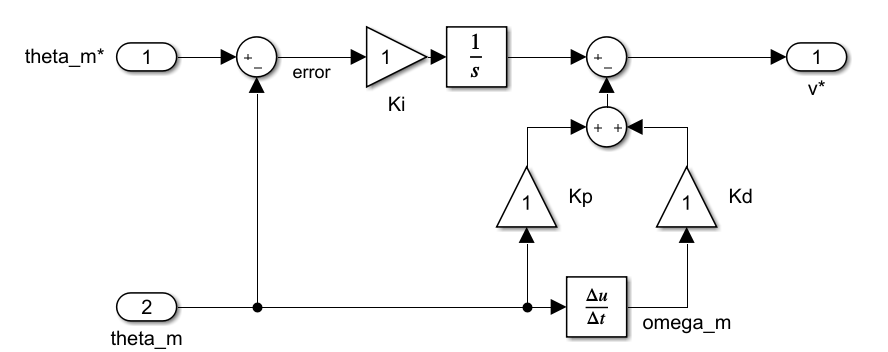
\includegraphics[width=0.60\textwidth]{Diagrama en bloques ilustrativo del controlador}
    \caption{Diagrama en bloques ilustrativo del controlador.}
    \label{fig:Diagrama en bloques ilustrativo del controlador}
\end{figure}

% Como se puede ver en la figura \ref{fig:Diagrama en bloques ilustrativo del controlador}, luego del bloque derivador se tiene la velocidad angular omega. Y como es conveniente no tener un bloque derivador (para evitar los problemas de amplificación de señal que conlleva la operación de derivación), se opta por eliminar este bloque derivador. Lo cual, es posible hacerlo si se puede realimentar el valor de la velocidad angular $\omega$. Pero, para ahorrar el tener que añadir un sensor de velocidad al sistema, y como se ha verificado la observabilidad de la planta, y al disponer de un modelo matemático de la misma, se puede estimar dicha variable de estado $\omega$ mediante un Observador de Estados. El observador es una copia de la planta que se agraga con la finalidad de recrear sus variables de estado. La figura \ref{fig:Incorporación del Observador de Estados al diagrama de bloques del sistema completo que se ha obtenido hasta el momento} muestra a modo de referencia, la incorporación del mismo en el diagrama de bloques del sistema completo que se ha obtenido hasta el momento:

% \begin{figure}[H]
%     \centering
%     \includegraphics[width=1\textwidth]{Incorporación del Observador de Estados al diagrama de bloques del sistema completo que se ha obtenido hasta el momento}
%     \caption{Incorporación del Observador de Estados al diagrama de bloques del sistema completo que se ha obtenido hasta el momento.}
%     \label{fig:Incorporación del Observador de Estados al diagrama de bloques del sistema completo que se ha obtenido hasta el momento}
% \end{figure}

% Entonces se tiene que, gracias a la implementación del observador, en el controlador I-PD no se necesita derivar la posición angular para obtener la velocidad $\omega$, sino que esta es estimada, es decir, recreada en el observador de estados. Por lo que el diagrama de control queda diseñado como se muestra en la figura \ref{fig:Diagrama en bloques del Control}.

% \begin{figure}[H]
%     \centering
%     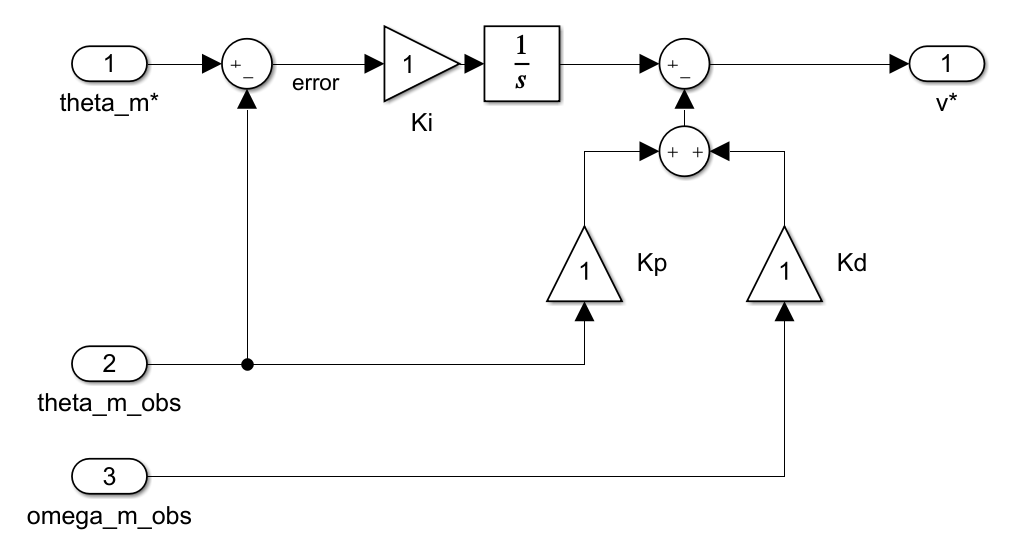
\includegraphics[width=0.60\textwidth]{Diagrama en bloques del Control}
%     \caption{Diagrama en bloques del Control.}
%     \label{fig:Diagrama en bloques del Control}
% \end{figure}

% Cabe aclarar que, el observador de estados y el controlador PID son ambos partes del controlador general de la articulación, y solo se muestran por separado para tener una vista simplificada.


\subsubsection{PLANIFICACIÓN DE GANANCIAS}
\label{sec:PLANIFICACIÓN DE GANANCIAS}

Debido a que la planta planta es un sistema LPV, como se mencionó, dicho controlador I-PD ha sido implementado en simulink mediante la técnica de planificación de ganancias.

Se tiene un única variable de planificación, que es el momento de inercia $J_l$, el cual lo ha dividido en cuatro valores igualmente separados por un paso fijo \ref{eq:Valores elegidos de Jl}. Este paso debe ser lo suficientemente pequeño como para obtener un buen desempeño del sistema en cualquier punto de todo su rango de operación; pero no demasiado pequeño porque mientras más pequeño sea, implica más puntos de operación en donde se tienen que ajustar las ganancias del PID, y tendríamos que ajustar demasiados controladores PID.

\paragraph{ETAPAS DEL DISEÑO DE UN PLANIFICADOR DE GANANCIAS:}
\label{sec:ETAPAS DEL DISEÑO DE UN PLANIFICADOR DE GANANCIAS:}
\hfill

\hfill

En términos generales, el diseño de un sistema de control de planificación de ganancias requiere de cuatro etapas:
\begin{enumerate}
    \item Linealizar la planta en cada punto de operación.
    \item Ajustar las ganancias del controlador PID en uno de estos puntos de operación.
    \item Implementar una arquitectura que planifique el mejor valor para cada ganancia del PID, en base al valor de la variable (o las variables) de planifición.

    Dicha arquitectura debe definir una curva de cada ganancia vs parámetro variable (o parámetros variables) que no posea saltos. Esto es debido a que, al ir cambiando el valor de una variable de planificación del sistema de forma continua, al cambiar de forma discreta las ganancias del PID, el error que se produce un salto discreto en la/s variable/s manipulada/s, lo que crea (un sacudón) oscilaciones no deseadas es la salida del sistema, al producirse un salto en el valor de la ganancia,esto produciría oscilaciones no deseadas (un sacudón) en la salida del sistema.
    En lugar de ello, dicha curva de cada ganancia vs parámetro variable debería corresponderse con alguna función polinómica, como líneas rectas que unan los valores del parámetro variable, o mejor aún, una curva más suave en el tiempo como  lo es una ecuación cuadrática.

    Cabe mencionar que si se tuvieran dos variables de planificación, entonces en lugar de una curva, se tendría una superficie. Y si se tuvieran más variables de planificación simplemente esta superficie se vuelve de orden mayor, y no es posible visualizarla fácilmente.
    %     - Herramientas SYS_TUNE y CONTROL_SYSTEM_TUNER de MATLAB and Simulink:
    %             Estas herramientas permiten:
    %                 - Elegir los puntos de operación de diseño.
    %                 - Definir la superficie de variables de planificación vs tiempo como una superfície polómica (mediante una ecuación).
    %                 - AJUSTAR (Tunear) AUTOMÁTICAMENTE LAS GANANCIAS DEL PID, en cada punto de operación de diseño. (ejemplo en descripción del video).
    \item Evaluar el desempeño del control en los diferentes posibles puntos de operación.

    % Esta evaluación conviene hacerla automáticamente por simulación, ya que es mucho más rápido que hacerla manualmente. Y claro que no se va a evaluar cada posible punto (ya que son demasiados, infinitos en la realidad) por lo que hay que elegir cuidadosamente cuáles puntos de operación evaluamos y cuales no. Hay que asegurarse que se evalúan todas las transiciones y los casos esquinas.
\end{enumerate}

\paragraph{IMPLEMENTACIÓN DEL PLANIFICADOR DE GANANCIAS:}
\label{sec:IMPLEMENTACIÓN DEL PLANIFICADOR DE GANANCIAS:}
\hfill

\hfill

Como ya se cuenta con una planta lineal para cada uno de los 4 puntos de operación considerados, se procede a ajustar las ganancias kp, ki y kd de cada uno de los controladores I-PD para cada una de las 4 plantas. Se hace uso de la función de MATLAB: $[C,info]=pidtune(sys,type,wc)$ para ajustar automáticamente los valores de las ganancias; junto con el bloque de simulink llamado: PID de 2 grados de libertad variable, y 3 tablas de búsqueda correspondientes a cada una de las 3 ganancias. Cada tabla de búsqueda realiza una interpolación lineal de los 4 valores de la ganancias ajustados. Así al recibir cualquier valor posible del parámetro variable $Jl$, entrega un valor correspondiente de la ganancia al bloque del controlador I-PD, como se muestra a continuación:

\begin{figure}[H]
    \centering
    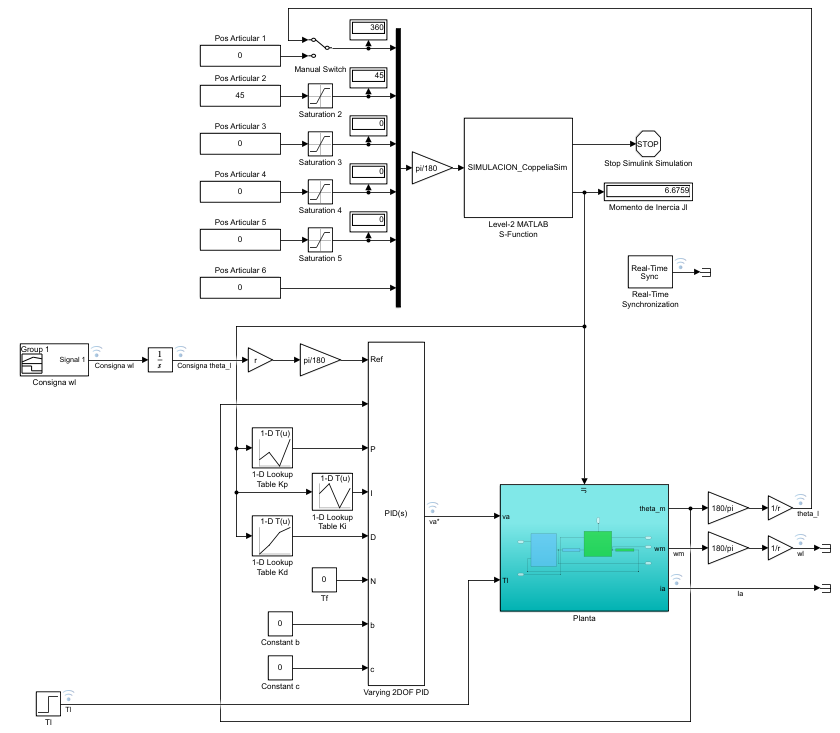
\includegraphics[width=1\textwidth]{Sistema Controlador-Planta}
    \caption{Sistema Controlador-Planta.}
    \label{fig:Sistema Controlador-Planta}
\end{figure}

Cabe mencionar que, luego de juntar la parte de arriba del modelo correspondiente al cálculo de $Jl$, con la parte de abajo del mismo correspondiente al controlador y bloque de la planta, la simulación comenzó a correr más lenta que el tiempo real. Entonces, se procedió a evalual el rendimiento del tiempo de ejecución del modelo mediante el \textbf{Profiler de Simulink}, con el cual se descubrió que la Función S de nivel 2 estaba realentizando al sistema debido a que se calculaba el momento de inercia $Jl$ en cada iteración. Por lo que se incorpocó un condicional if para que solo lo calcule cuando alguna posición angular (que no sea de la articulación base) de consigna, no coincida con la posición angular corresondiente del robot en la simulación de CoppeliaSim.

Y luego de realizar este ajuste en el código, la simulación en Simulink corría más rápido que el tiempo real, con lo que instaló el kernel de tiempo real de simulink y Se incorporó al modelo, el bloque llamado: sincronización de tiempo real .

Por otro lado, mediante la información devuelta por la función pidtune de MATLAB, mediante código de MATLAB se corroboró la estabilidad de los 4 sistemas controlador-planta:

\begin{figure}[H]
    \centering
    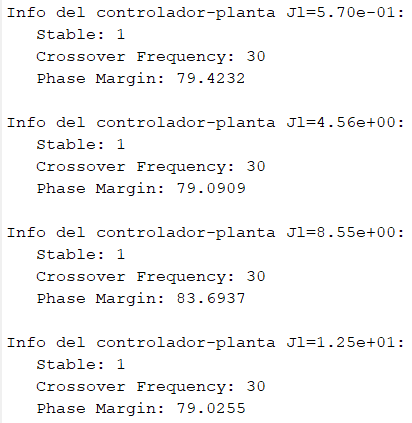
\includegraphics[width=0.4\textwidth]{Información de vuelta por la función pidtune de MATLAB}
    \caption{Información de vuelta por la función pidtune de MATLAB.}
    \label{fig:Información de vuelta por la función pidtune de MATLAB}
\end{figure}


\paragraph{RESPUESTA DEL SISTEMA CONTROLADOR-PLANTA:}
\label{sec:RESPUESTA DEL SISTEMA CONTROLADOR-PLANTA:}
\hfill

\hfill

Para evaluar la respuesta del sistema controlador-planta, se toma como referencia una consigna de $\omega_l$ tapezoidal, la cual se la integra para obtener una consigna de $\theta_l$ que describe una rampa suave en el tiempo desde cero a 360°. Y además a los 6 segundos se aplica el $T_{l_{\text{máx}}}=330 ~N.m$.

La respuesta se evalúa para tres valores del parámetro variable: su valor mínimo, su valor máximo, y un valor $J_l=6,6261 ~kg.m^2$ el cual es un valor intermedio de los 4 puntos de operación tomados para el diseño de los respectivos 4 controladores I-PD:
\begin{figure}[H]
    \centering
    \includegraphics[width=1\textwidth]{Los 3 puntos de operación evaluados}
    \caption{Los 3 puntos de operación evaluados.}
    \label{fig:Los 3 puntos de operación evaluados}
\end{figure}

\begin{figure}[H]
    \centering
    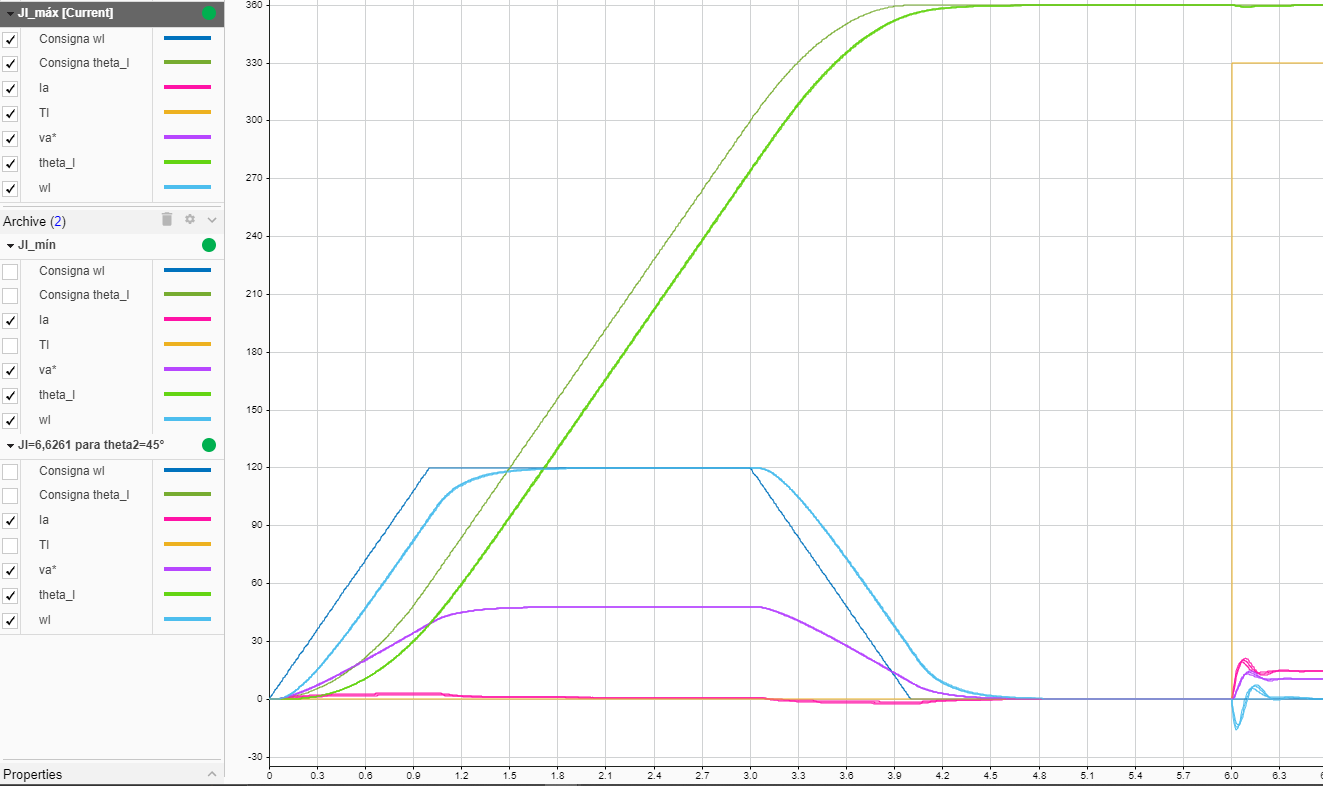
\includegraphics[width=1\textwidth]{Respuesta del sistema controlador-planta}
    \caption{Respuesta del sistema controlador-planta.}
    \label{fig:Respuesta del sistema controlador-planta}
\end{figure}

\begin{figure}[H]
    \centering
    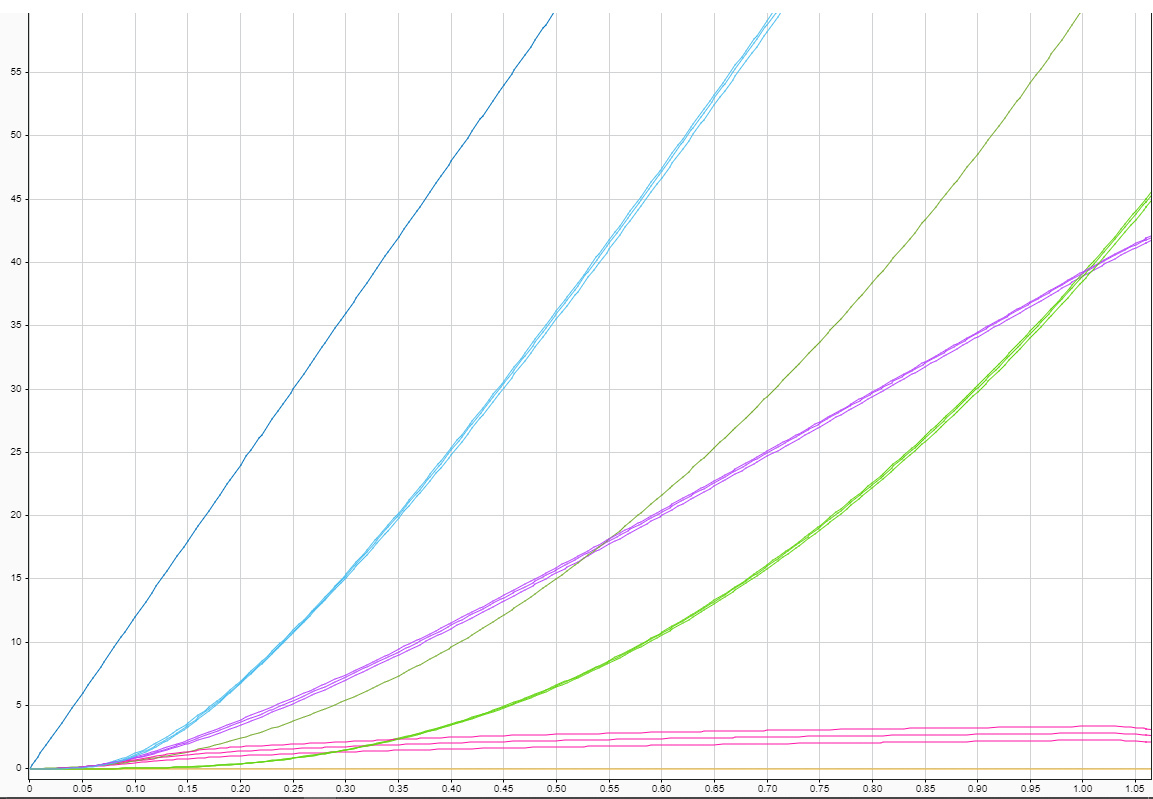
\includegraphics[width=1\textwidth]{Zoom de la respuesta a la consigna trapezoidal de velocidad integrada, del sistema controlador-planta}
    \caption{Zoom de la respuesta a la consigna trapezoidal de velocidad integrada, del sistema controlador-planta.}
    \label{fig:Zoom de la respuesta a la consigna trapezoidal de velocidad integrada, del sistema controlador-planta}
\end{figure}

\begin{figure}[H]
    \centering
    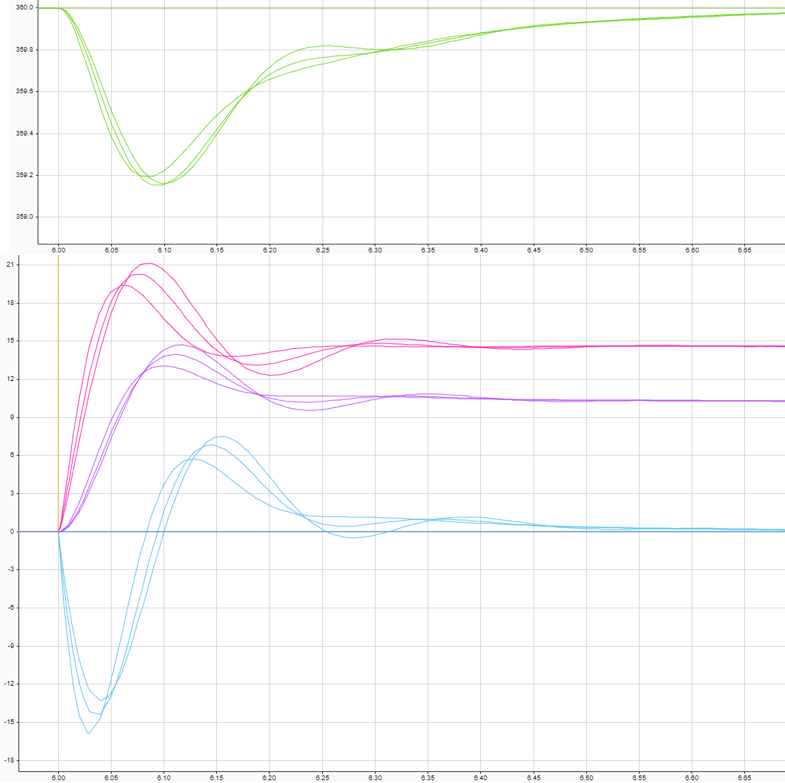
\includegraphics[width=1\textwidth]{Zoom de la respuesta a la pertubación escalón del sistema controlador-planta}
    \caption{Zoom de la respuesta a la pertubación escalón del sistema controlador-planta.}
    \label{fig:Zoom de la respuesta a la pertubación escalón del sistema controlador-planta}
\end{figure}

Además se aprecian los siguentes valores de $v_a$ e $i_a$ y la variación máxima de $\theta_l$ al aplicar la carga:

\begin{table}[H]
    \centering
    \begin{tabular}{|l|l|l|l|}
    \cline{1-4}
    \textbf{$J_{l_{\text{mín}}}$}        & $i_{a_{\text{máx}}} ~[A]$ & $v_{a_{\text{máx}}} ~[V]$ & $\Delta\theta_l$° \\\cline{1-4}
    \textbf{Respuesta a la referencia}   & 2,3                       & 47,9                      & -                 \\\cline{1-4}
    \textbf{Respuesta a la perturbación} & 19,4                      & 13,1                      & 0,8               \\\cline{1-4}
    \end{tabular}
    \caption{\label{table:Valores de la respuesta del sistema controlador-planta para Jlmín}Valores de la respuesta del sistema controlador-planta para $J_{l_{\text{mín}}}$.}
\end{table}

\begin{table}[H]
    \centering
    \begin{tabular}{|l|l|l|l|}
    \cline{1-4}
    \textbf{$J_l=6,6261 ~kg.m^2$}        & $i_{a_{\text{máx}}} ~[A]$ & $v_{a_{\text{máx}}} ~[V]$ & $\Delta\theta_l$° \\\cline{1-4}
    \textbf{Respuesta a la referencia}   & 2,8                       & 47,9                      & -                 \\\cline{1-4}
    \textbf{Respuesta a la perturbación} & 20,2                      & 13,9                      & 0,8               \\\cline{1-4}
    \end{tabular}
    \caption{\label{table:Valores de la respuesta del sistema controlador-planta para Jl=6,6261}Valores de la respuesta del sistema controlador-planta para $J_l=6,6261 ~kg.m^2$.}
\end{table}

\begin{table}[H]
    \centering
    \begin{tabular}{|l|l|l|l|}
    \cline{1-4}
    \textbf{$J_{l_{\text{máx}}}$}        & $i_{a_{\text{máx}}} ~[A]$ & $v_{a_{\text{máx}}} ~[V]$ & $\Delta\theta_l$° \\\cline{1-4}
    \textbf{Respuesta a la referencia}   & 3,3                       & 47,9                      & -                 \\\cline{1-4}
    \textbf{Respuesta a la perturbación} & 21,1                      & 14,7                      & 0,8               \\\cline{1-4}
    \end{tabular}
    \caption{\label{table:Valores de la respuesta del sistema controlador-planta para Jlmáx}Valores de la respuesta del sistema controlador-planta para $J_{l_{\text{máx}}}$.}
\end{table}


Se puede observar que el sistema no conserva ningún error de estado estacionario al cesar el cambio de consigna, pero si se observa un error de estado estacionario cuando la consigna (tanto de velocidad como de posición angular) se encuentra describiendo una rampa. El valor máximo de error estacionario ante la  consigna rampa de $\theta_l$ correspondiente al $J_{l_{\text{máx}}}$ es de 27°, y el desfasaje del robot con la rampa de consigna es de solo 0,22 s el cual es un tiempo aceptable para la aplicación. Aunque dicho error de estado estacionario se podría eliminar agregando un integrador puro al sistema.














% ======================================================================
\subsection{PROCESAMIENTO DE SEÑALES}
\label{sec:PROCESAMIENTO DE SEÑALES}


\subsubsection{INCORPORACIÓN DE RUIDO EN LA PLANTA}
\label{sec:INCORPORACIÓN DE RUIDO EN LA PLANTA}

A continuación, se incorpora ruido al proceso. Esto sirve para representar a las perturbaciones o fluctuaciones no controladas que afectan al sistema dinámico, las cuales pueden surgir de diversas fuentes, como errores en el modelo matemático utilizado para describir el sistema, influencias ambientales, la variabilidad inherente del sistema o cualquier otra fuente de incertidumbre.

El ruido del proceso se modela como una señal aleatoria que se suma al modelo dinámico del sistema. Con lo que el sistema en el espacio de estados \ref{eq:modelo completo de la planta en forma matricial} se convierte en:

\begin{align} \label{eq:modelo completo de la planta en forma matricial con ruido}
    \begin{cases}
        \dot{x}\left(t\right)=A.x\left(t\right)+B.u\left(t\right)+v\left(t\right)
        \\
        y(t)\ =\ C.\ x(t)
    \end{cases}
\end{align}

En donde $v(t)$ es un vector 3x1 de variables con media cero y varianza de $1\times10^{-3}$.

\begin{figure}[H]
    \centering
    \includegraphics[width=0.35\textwidth]{Generación del ruido del proceso}
    \caption{Generación del ruido del proceso.}
    \label{fig:Generación del ruido del proceso}
\end{figure}

\begin{figure}[H]
    \centering
    \includegraphics[width=1\textwidth]{Incorporación del ruido del proceso}
    \caption{Incorporación del ruido del proceso.}
    \label{fig:Incorporación del ruido del proceso}
\end{figure}

\begin{figure}[H]
    \centering
    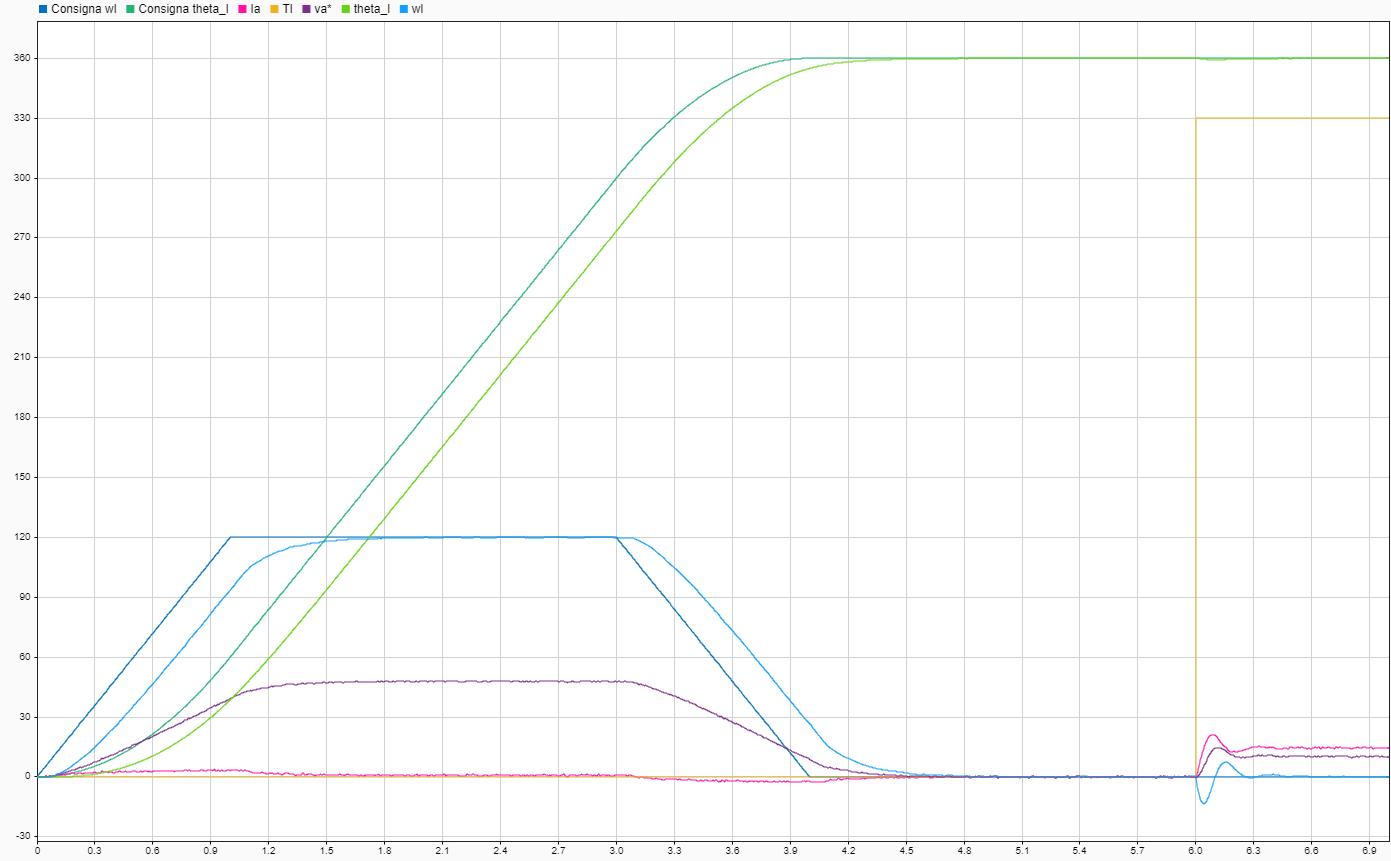
\includegraphics[width=1\textwidth]{Respuesta del Sistema con Ruido del proceso}
    \caption{Respuesta del Sistema con Ruido del proceso.}
    \label{fig:Respuesta del Sistema con Ruido del proceso}
\end{figure}

\begin{figure}[H]
    \centering
    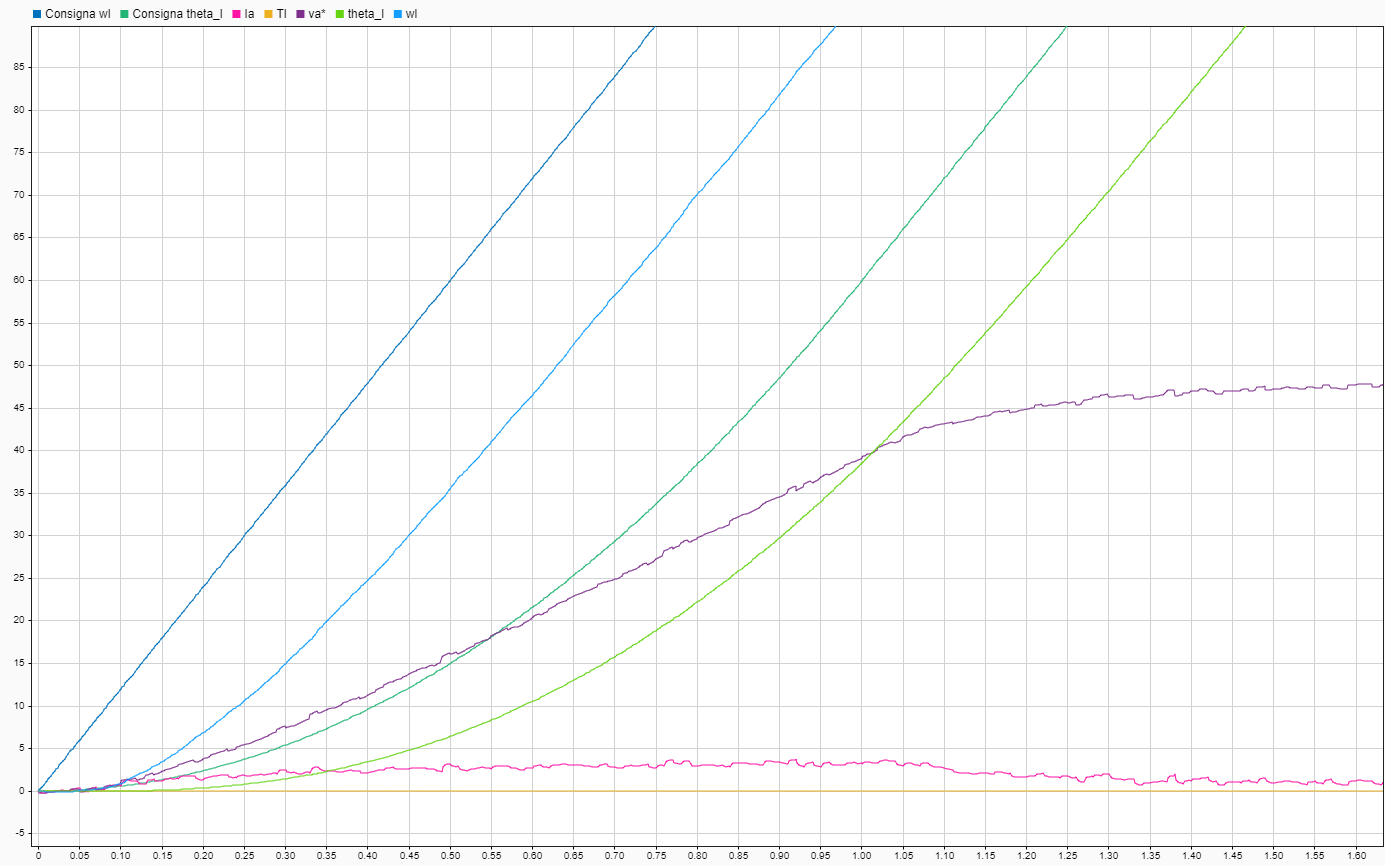
\includegraphics[width=1\textwidth]{Acercamiento de la respuesta del Sistema con Ruido del proceso}
    \caption{Acercamiento de la respuesta del Sistema con Ruido del proceso.}
    \label{fig:Acercamiento de la respuesta del Sistema con Ruido del proceso}
\end{figure}

\subsubsection{INCORPORACIÓN DE RUIDO EN EL SENSOR}
\label{sec:INCORPORACIÓN DE RUIDO EN EL SENSOR}

A continuación, también se incopora el sensor de la salida a ser realimenta, modelándolo con ruido para obtener una simulación más realista del sistema, con el cual se conseguirá robustecer el control.

Como sensor para medir la posición angular de la articulación del robot se dispone de un encoder absoluto. El cual, comparado con un encoder incremental, tiene la ventaja de que puede medir la posición absoluta del eje en cualquier momento, incluso luego de un corte en el suministro de energía eléctrica, sin necesidad de tener que recalibrarlo. Esta robustez en la determinación de la posición absoluta es fundamental para un cobot, por motivos de seguridad. Además dicha ventaja lo hace más robusto en su cuenta de pulsos, los cuales en un encoder incremental es más común tener la pérdida de algún pulso o contar un pulso falso, debido a diferentes factores, como la contaminación del disco del codificador, la exposición a interferencias electromagnéticas, vibraciones mecánicas y fluctuaciones en la fuente de alimentación, entre otras.

Como encoder absoluto se selecciona el AD58S DRIVE-CLiQ de la empresa Hengstler \cite{Absolute_Encoder_Datasheet}, el cual es del tipo óptico, y posee una resolución monovuelta de 24 bits \ref{fig:Datasheet del encoder}. Dicha resolución, se corresponde con una precisión de $+-35''=+-\frac{7}{720}\text{°}=+-0,0097\overline{2}$°.

\begin{figure}[H]
    \centering
    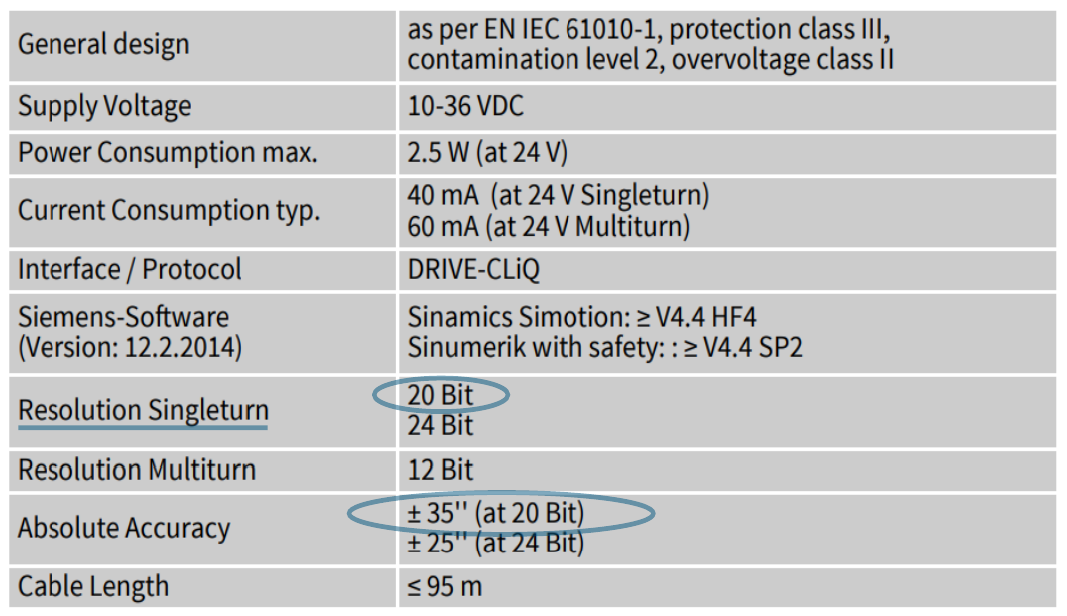
\includegraphics[width=0.5\textwidth]{Datasheet del encoder}
    \caption{Datasheet del encoder.}
    \label{fig:Datasheet del encoder}
\end{figure}

Como el encoder se coloca entre el motor y el reductor, entonces la precisión para el eje de salida del reductor termina siendo: $+-\frac{0,58\overline{3}\text{°}}{r}=+-0,000060763$°

Y se tiene que para el alcance máximo de $1,300 ~m$ del brazo robótico, y una repetibilidad del mismo de $+-0,0001 ~m$, aplicando el teorema del coseno \ref{fig:Aplicación del teorema del coseno para obtener la precisión del robot en grados}, se obtiene una precisión angular de $+-0,0044$°. La cual, al multiplicarse por r=160 se obtiene una precisión angular en el eje del motor igual a: $+-0,0044\text{°}=0,704$°. Y, al ser esta presición nescesaria mayor que la precisión que posee el encoder, se puede intuir que dicho sensor de posición seleccionado es adecuado.

Cabe aclarar, que si se controlaran todas las articulaciones del robot, habría que recalcular la precisión angular, considerando la contribución de las demás articulaciones en la configuración articular más desfavorable del robot.

\begin{figure}[H]
    \centering
    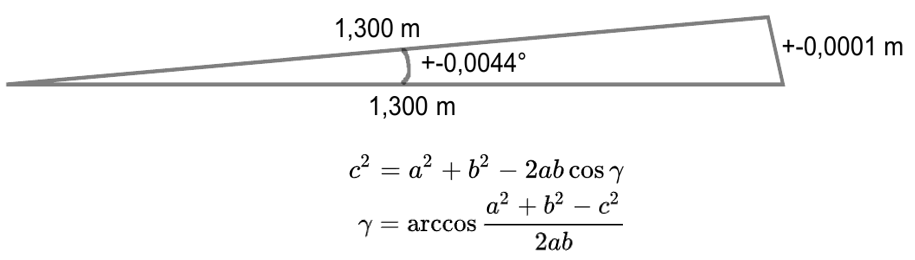
\includegraphics[width=0.8\textwidth]{Aplicación del teorema del coseno para obtener la precisión del robot en grados}
    \caption{Aplicación del teorema del coseno para obtener la precisión del robot en grados.}
    \label{fig:Aplicación del teorema del coseno para obtener la precisión del robot en grados}
\end{figure}

Al sensor se lo modelo como un conversor A/D, al cual se le agrega ruido para simular la precisión especificada en la hoja de datos.

\begin{figure}[H]
    \centering
    \includegraphics[width=0.4\textwidth]{Conversor Analógico Digital}
    \caption{Conversor Analógico Digital.}
    \label{fig:Conversor Analógico Digital}
\end{figure}

\paragraph{Primera Etapa del Modelo de un Conversor A/D:}
\label{sec:Primera Etapa del Modelo de un Conversor A/D:}
\hfill

\hfill

La primera etapa del modelo consiste en el muestreo y retención (en inglés: sample and hold) de la señal de salida continua y variable en el tiempo $x(t)$, proveniente del sistema.

El objetivo de esta primera etapa, es simplemente el del mantener por un tiempo determinado un valor típicamente de tensión a la entrada del conversor A/D. Lo cual es necesario ya que el conversor A/D no puede realizar la conversión del valor de tensión a un valor binario de forma instantánea, sino que le toma un cierto tiempo finito distinto de cero. Cabe aclarar que para el caso de un encoder absoluto físico, este no utiliza un valor de tensión proporcional a la variable que mide, sino que realiza el muestreo y retención físicamente, con el propio mecanismo con el que funciona.

La etapa de muestreo y retención se la simula en Simulink mediante un retenerdor de orden cero, bloque llamado: zero-order hold (ZOH), al cual se le ingresa como parámetro el periodo de muestreo T. El valor de T se obtiene al extraer la variable de salida $\theta_m$, de la cual se obtiene el vector de tiempo tout de dicha señal. Y si se comprueba que paso de tiempo $\Delta t$ de dicho vector se mantiene igual, entonces se utiliza este como tiempo de muestreo en el bloque ZOH. Así se obtuvo un período $T=\Delta t=0,01s$.

\paragraph{Segunda Etapa del Modelo de un Conversor A/D:}
\label{sec:Segunda Etapa del Modelo de un Conversor A/D:}
\hfill

\hfill

La segunda etapa consiste en el conversor A/D propiamente dicho, al cual a su vez se lo divide en tres subetapas:

\begin{figure}[H]
    \centering
    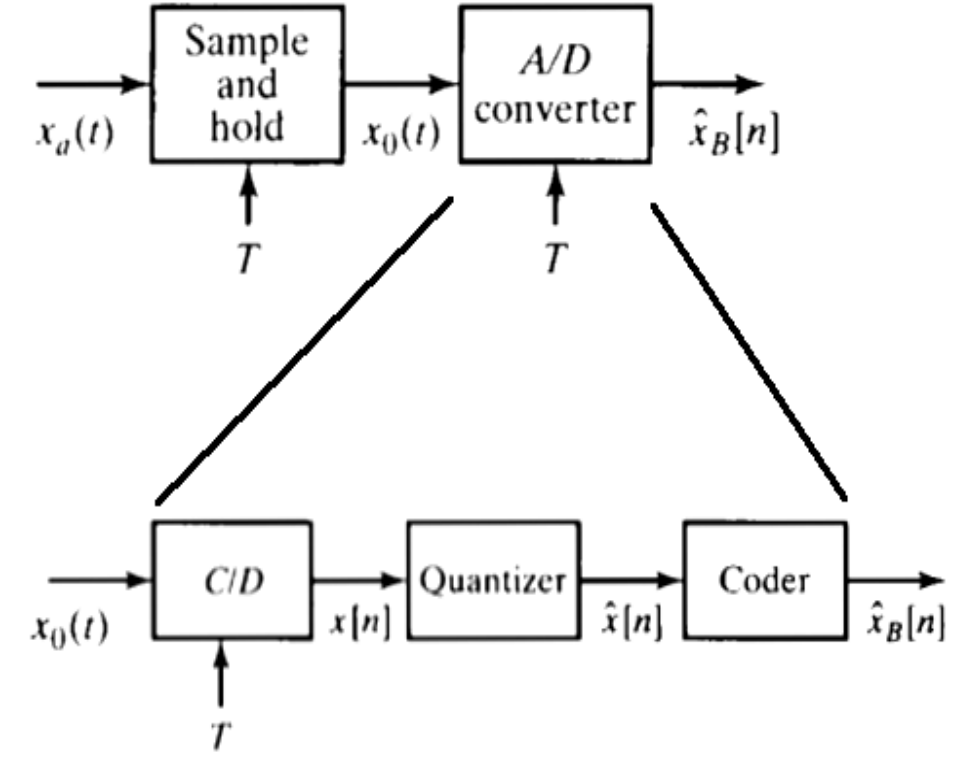
\includegraphics[width=0.4\textwidth]{Tres subetapas del conversor AD propiamente dicho}
    \caption{Tres subetapas del conversor A/D propiamente dicho.}
    \label{fig:Tres subetapas del conversor A/D propiamente dicho}
\end{figure}

El subbloque C/D muestrea (discretiza) el valor continuo de tensión mantenida constante, correspondiente de la variable $x_0(t)$ a medir, a un solo valor (discreto) x[t].

Luego, el bloque cuantizador toma el valor discretizado x[t], y le da un valor $\hat{x}[t]$ correspondiente a uno de valores de los que le es posible representar, los cuales dependen de la cantidad de bits que tenga el conversor A/D. Y al hacerlo, se tiene que este subbloque introduce ruido, debido a la misma cuantificación de la señal.

Finalmente, el bloque codificador toma al valor valor $\hat{x}[t]$, y lo acomoda a un tipo de sistema de numeración deseado (como binario con o sin signo, complemento A2, o punto flotante, entre otros), obteniendo un valor $\hat{x_B}[t]$ representado en dicho sistema de numeración.

\paragraph{Obtención del Ruido que genera el Encoder:}
\label{sec:Obtención del Ruido que genera el Encoder:}
\hfill

\hfill

El ruido aportado por el encoder se simula como ruido Gaussiano, con media cero y varianza:

\begin{subequations} \label{eq:Cálculo de la Varianza correspondiente al ruido aportado por la precisión del sensor}
	\begin{align}
        \sigma_{sensor}^2=\varphi_{\text{precisión}}^2
        \\
        \sigma_{sensor}^2=(0,0097\overline{2}\text{°}.\frac{\pi ~rad}{180\text{°}})^2
        \\
        \label{eq:Varianza} \sigma_{sensor}^2=2,89\times10^{-8} ~[rad^2]
	\end{align}
\end{subequations}

Este ruido se lo modela como ruido blanco Gaussiano, mediante el bloque de Simulink llamado: Band-Limited White Noise. A dicho bloque, se le ingresa como parámetro varianza previamente calculada.

A continuación se muestra el diagrama en bloques del modelo del sensor modelado, con el que se obteniene la salida censada del sistema:

\begin{figure}[H]
    \centering
    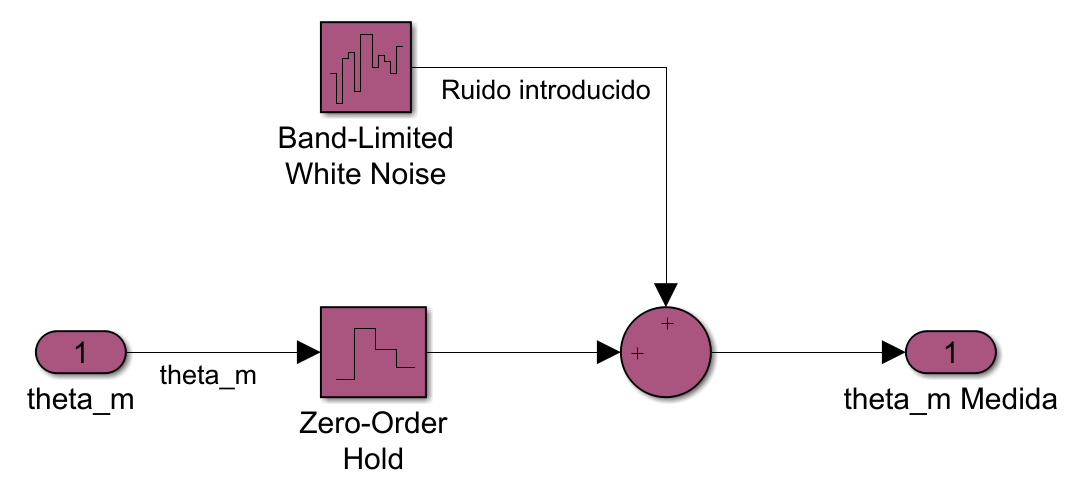
\includegraphics[width=0.5\textwidth]{Diagrama en bloques del modelo del sensor obtenido}
    \caption{Diagrama en bloques del modelo del sensor obtenido.}
    \label{fig:Diagrama en bloques del modelo del sensor obtenido}
\end{figure}

Y en la siguiente figura se muestra el ruido introducido por el sensor:

\begin{figure}[H]
    \centering
    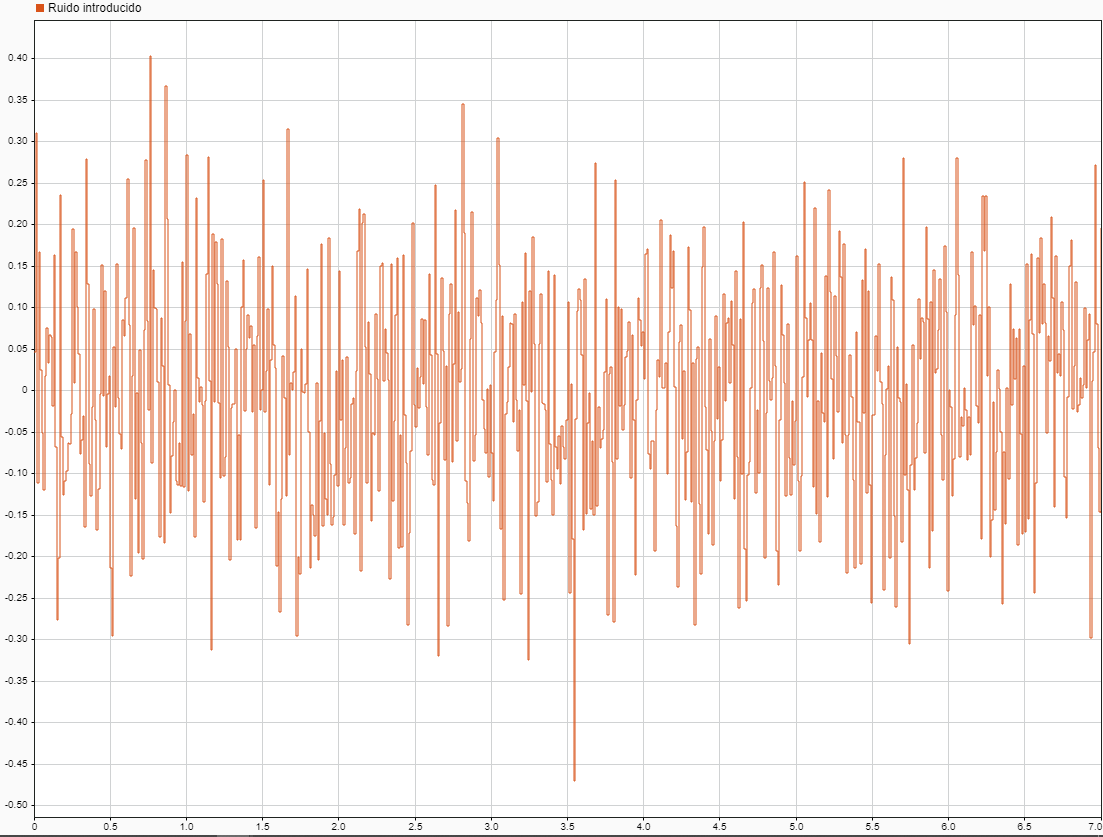
\includegraphics[width=1\textwidth]{Salida del sensor para una consigna nula}
    \caption{Salida del sensor para una consigna nula.}
    \label{fig:Salida del sensor para una consigna nula}
\end{figure}

Para mitigar este ruido, se utilizará el filtro de Kalman, el cual se describe a continuación.


\subsubsection{FILTRO DE KALMAN DISCRETO}
\label{sec:FILTRO DE KALMAN DISCRETO}

Se escogió al filtro de Kalman como observador de estados para estimar el valor del ángulo del motor $\theta_m(t)$, el cual que se realimenta al controlador, debido a que al ser el sistema lineal, y al involucrar solo ruido con distribución Gaussiana, entonces el filtro de Kalman el mejor estimador de estados posible. Esto es debido a que el mismo trata de
encontrar los valores de los estados 'x' y de la/s salida/s 'y', a partir de minimizar el error entre los valores de los estados estimados $\hat{x}(t)$, y los valores reales de los estados $x(t)$ del sistema.

Por otro lado, cabe notar que como el sistema es observable, entonces el filtro de kalman va a ser estable.

El filtro de kalman considera el siguiente sistema de ecuaciones:

\begin{align} \label{eq:sistema de ecuaciones Del filtro de Kalman}
    \begin{cases}
        x[k+1]=A.x[k]+B.u[k]+v[k]
        \\
        y[k]=C.x[k]+w[k]
    \end{cases}
\end{align}

Dónde dónde w representa el ruido de medición, y v el ruido del proceso. En donde se supone que ambos ruidos siguen una distribución Gaussiana con media igual a 0. (Si se tuviera ruido con una distribución distinta se debería utilizar otro tipo de filtro de Kalman (distinto al estandar), como lo es el filtro de Kalman de Partículas).

Los parámetros del diseño del filtro de Kalman son las matrices de covarianzas $R_v$ $R_w$, las cuales representan respectivamente al ruido del proceso y ruido de medición.

Al disponerse de 3 variables de estado, entonces la matriz $R_v$ es de dimensión 3x3, y es una matriz diagonal cuyos valores son iguales a las varianzas del ruido ingresado en las 3 variables de estado:

\begin{align}
    R_v=\left[\begin{matrix}1\times{10}^{-3}&0&0\\0&1\times{10}^{-3}&0\\0&0&1\times{10}^{-3}\\\end{matrix}\right]
\end{align}

Por otro lado, al disponerse de solo una variable a medir, entonces la matriz de covarianza $R_w$ correspondiente al ruido del sensor se convierte en un escalar, y es igual al valor de la varianza calculada en la sección \ref{sec:INCORPORACIÓN DE RUIDO EN EL SENSOR}:

\begin{align}
    R_w=2,89\times10^{-8} %~[rad^2]
\end{align}

La covarianza del error de estimación $P_{{x}}[k+1]$ es:

\begin{align}
    P_{\widetilde{x}}\left[k+1\right]=\left(A-L\left[k\right].C\right){.P}_{\widetilde{x}}\left[k\right].\left(A-L\left[k\right].C\right)^T+R_v+L\left[k\right].R_w.L^T\left[k\right]
\end{align}

Y la ganancia óptima del observador es:

\begin{align}
    L\left[k\right]=A{.P}_{\widetilde{x}}\left[k\right].C^T\left(R_W+C{.P}_{\widetilde{x}}\left[k\right].C^T\right)^{-1}
\end{align}

Es importante notar que el filtro de Kalman Discreto es un filtro recursivo, lo que implica que en cada paso de timpo se calcula el estado estimado y la ganancia óptima L.

Existen diferentes enfoques algorítmicos para la implementación del filtro. Para el proyecto actual se eligió el bloque de Simulink: Kalman Filter.

\begin{figure}[H]
    \centering
    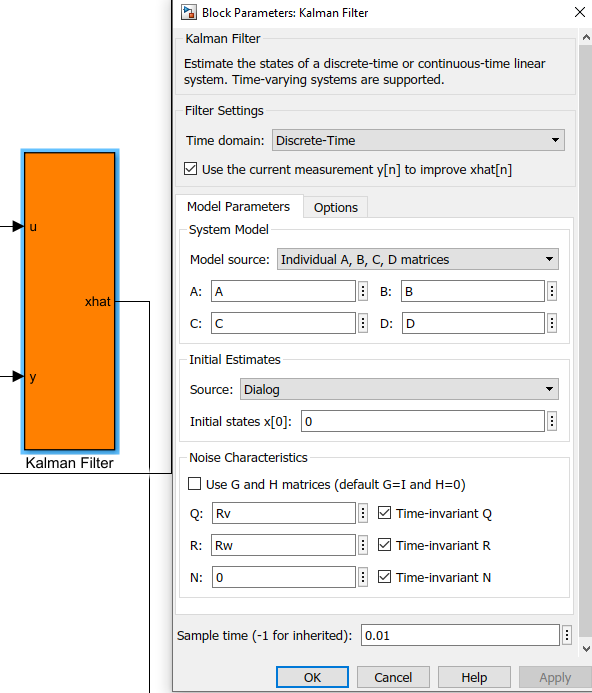
\includegraphics[width=0.7\textwidth]{Bloque del filtro de Kalman en Simulink, y su configuración de parámetros}
    \caption{Bloque del filtro de Kalman en Simulink, y su configuración de parámetros.}
    \label{fig:Bloque del filtro de Kalman en Simulink, y su configuración de parámetros}
\end{figure}

% El proceso de estimación del filtro de Kalman puede resumirse en los siguientes pasos:

% Inicialización: Se establece el estado inicial del sistema y se define la matriz de covarianza del error de estimación inicial.

% Predicción: Se predice el nuevo estado del sistema y se calcula la matriz de covarianza de predicción utilizando el modelo dinámico del sistema y la matriz de covarianza del proceso de ruido.

% Actualización (Corrección): Se obtiene una nueva estimación del estado del sistema utilizando la medida más reciente, combinándola con la predicción anterior y su covarianza mediante el teorema de Bayes. Esto se realiza mediante la matriz de ganancia de Kalman, que determina cuánto peso se debe dar a la predicción y cuánto a la medida.

% Repetición: Se repiten los pasos de predicción y actualización para cada nueva medida recibida, refinando continuamente la estimación del estado del sistema.

% -----------------------------------------------------------------------
% El filtro de Kalman calcula la matriz L considerando que el sistema está afectado por ruido.




% A MEDIDA QUE EL VALOR DEL RUIDO AUMENTA, EL FILTRO DE KALMAN TARDA MÁS EN ESTIMAR EL VALOR DE x1.

El diagrama en bloques del sistema completo obtenido es:

\begin{figure}[H]
    \centering
    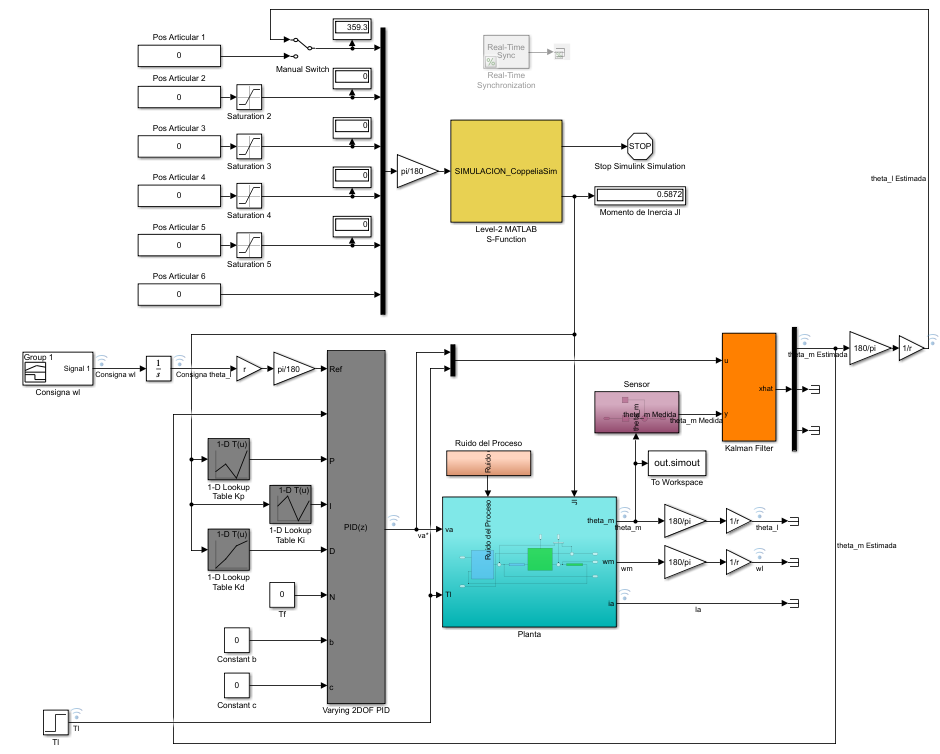
\includegraphics[width=1\textwidth]{Diagrama de Bloques del Sistema Completo}
    \caption{Diagrama de Bloques del Sistema Completo.}
    \label{fig:Diagrama de Bloques del Sistema Completo}
\end{figure}







% \paragraph{FUNDAMENTO DE LA UTILIZACIÓN DE UN CONTROLADOR DISCRETO:}
% \label{sec:FUNDAMENTO DE LA UTILIZACIÓN DE UN CONTROLADOR DISCRETO:}
% \hfill

% \hfill
%%%%%%%%%%%%%%%%%RESUMIR: $https://www.youtube.com/watch?v=14cMhrp5wlk$





% \paragraph{SELECCIÓN DEL TIPO DE MÉTODO DE DISCRETIZACIÓN:}
% \label{sec:SELECCIÓN DEL TIPO DE MÉTODO DE DISCRETIZACIÓN:}
% \hfill

% \hfill

% En MATLAB se utiliza la función \cite{c2d}: \textbf{SYSD = c2d(SYSC, TS, METHOD)} para obtener el modelo discreto SYSD, con tiempo de muestreo TS, de un modelo continuo SYSC, mediante el uso del método METHOD, el cual puede ser uno de los siguientes métodos:
% \begin{description}
%     \item ['\textbf{zoh}':] Retención de Orden Cero (siglas del inglés: zero-order hold) o Discretización Invariante al Escalón.
%     \item ['\textbf{foh}':] Retención de Primer Orden (siglas del inglés: first-order hold) o Aproximación Triangular.
%     \item ['\textbf{impulse}':] Discretización de Impulso Invariante.
%     \item ['\textbf{tustin}':] Transformación Bilineal (Tustin).
%     \item ['\textbf{matched}':] Método de Correspondencia de Polos y Ceros.
%     % \item ['\textbf{least-squares}':] Método de Mínimos Cuadrados.
% \end{description}

% Dichos métodos, convierten a un sistema continuo en un sistema discreto, o bien como suele ser el caso, convierten a un filtro analógico en el dominio S en un filtro digital en el dominio Z.
% Cada uno de los métodos da lugar a una función de transferencia en el dominio Z, la cual es distinta para los distintos métodos. Para un sistema dado, la función de transferencia obtenida siempre posee la misma ecuación característica sin importar el método utilizado, lo que significa que siempre se obtienen unos mismos polos y por lo tanto una misma estabilidad. Pero los ceros de dicha función de transferencia son distintos para cada método. Esto provoca que el modelo discreto obtenido por un método, presente una respuesta con ciertas diferencias respecto a los demás métodos. Por ejemplo, para un modelo con función de transferencia: $G(S)=\frac{1}{S+1}$, se obtiene para cada método la respuesta del modelo discretizado, tanto en el dominio del tiempo como en dominio de la frecuencia, \ref{fig:Diferencias en la respuesta que produce cada método para un modelo dado}:

% \begin{figure}[H]
%     \centering
%     \includegraphics[width=1\textwidth]{Diferencias en la respuesta que produce cada método para un modelo dado}
%     \caption{Diferencias en la respuesta que produce cada método para un modelo dado.}
%     \label{fig:Diferencias en la respuesta que produce cada método para un modelo dado}
% \end{figure}

% Las diferencias entre cada método están dadas por el hecho de que cuando un sistema se discretiza, inevitablemente se pierde algo de información al muestrear el sistema continuo. Y cada método se enfoca en minimizar la pérdida de cierta información del sistema por sobre otra. Por lo que la elección del método depende de qué información se desea conservar, lo que depende de qué se desea lograr.
% Por ejemplo, el \textbf{método (impulse) de impulso invariante}, logra que la respuesta del sistema a un impulso sea prácticamente idéntica a la repuesta que tiene el sistema continuo ante el mismo impulso. Mientras que, por ejemplo el \textbf{método (zoh) del retención de orden cero}, no produce una respuesta tan certera al impulso, sino que se enfoca en lograr que coincida la respuesta ante un escalón del sistema discretizado, con la repuesta ante el mismo escalón del sistema continuo \ref{fig:Comparación de la respuesta ante un escalón, entre modelo continuo dado y su discretización utilizando el método del impulso y el método de zoh respectivamente}. Debido a ello, al método zoh también se lo suele llamar: método de escalón invariante.

% % [[[[[[[[[Ahora, como la consigna de referencia que se comanda para controlar a un motor, en general mantiene su valor en el tiempo hasta que el controlador recibe otro valor de la consigna de referencia. Entonces lo que se desea lograr al discretizar el controlador, es mantener la respuesta del sistema ante escalones de consigna. Por lo que se elige trabajar con el método zoh.]]]]]]]]]%%%%%%%%%% RESUMIR PORQUÉ NO SE UTILIZA EL MÉTODO DE ZOH: https://www.youtube.com/watch?v=yetLPW9sQaI&list=PLUMWjy5jgHK0MLv6Ksf-NHi7Ur8NRNU4Z&index=5

% \begin{figure}[H]
%     \centering
%     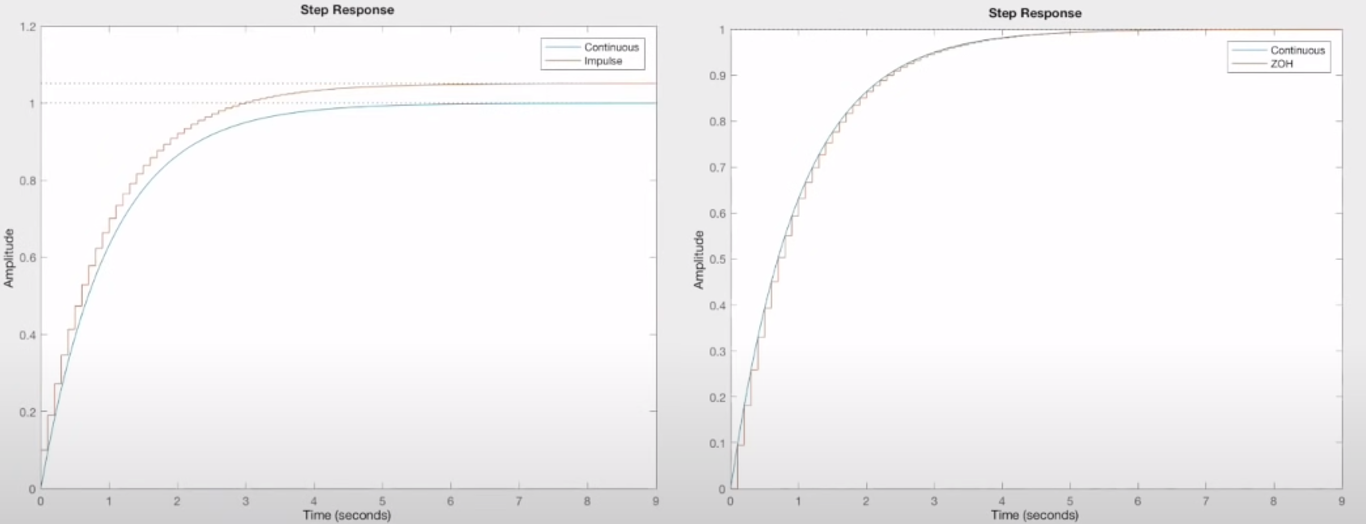
\includegraphics[width=1\textwidth]{Comparación de la respuesta ante un escalón, entre modelo continuo dado y su discretización utilizando el método del impulso y el método de zoh respectivamente}
%     \caption{Comparación de la respuesta ante un escalón, entre modelo continuo dado y su discretización utilizando el método del impulso y el método de zoh respectivamente.}
%     \label{fig:Comparación de la respuesta ante un escalón, entre modelo continuo dado y su discretización utilizando el método del impulso y el método de zoh respectivamente}
% \end{figure}

% Por otro lado, el \textbf{método (foh) de retención de primer orden}, es similar al método zoh, solo que en lugar de mantenener el último valor muestreado constante, mantiene la pendiente constante, produciendo una serie de rampas en lugar de una serie de escalones como en el zoh. Por ello, el método foh conserva la respuesta ante una rampa de entrada, y por ello se lo suele también llamar método de rampa invariante.

% Los tres métodos mencionados (zoh, foh e impulse) producen una respuesta en el tiempo precisa, respectivamente ante una entrada de escalón, rampa o impulso. Sin embargo, el \textbf{método (matched) de correspondencia de polos y ceros}, no trata de tener una respuesta precisa en el tiempo como su contraparte en el dominio S, ni siquiera produce una respuesta en la frecuencia simular. Por esto, el método matched además de ser solo aplicable para sistemas SISO, es como mucho solo un recurso provisional y prácticamente no es utilizado, sino que se prefiere utilizar otro de los métodos. Sino que este método se enfoca en responder a la pregunta: ¿qué ocurre si se mueve cada polo y cero en el dominio S, a su correspondiente lugar en el dominio Z?

% Y por último se tiene al método más usado, que es el \textbf{método (tustin) de transformación bilineal}, formulado por el ingeniero británico Arnold Tustin. El cual consiste en reemplazar la variable S de laplace por la transformación bilineal dada por siguiente ecuación :

% \begin{align}   \label{eq:Transformación Bilineal}
%     S=\frac{2}{T}.\left(\frac{Z-1}{Z+1}\right)
% \end{align}

% Donde T es el tiempo de muestreo. Y al despejar la variable Z, se obtiene la transformación bilineal inversa:

% \begin{align}   \label{eq:Transformación Bilineal Inversa}
%     Z=\frac{1+\frac{T}{2}.S}{1-\frac{T}{2}.S}
% \end{align}

% En la cual \ref{eq:Transformación Bilineal Inversa}, al reemplazar la variable S por el valor de un polo o cero en el plano-S de un sistema, se puede obtener el correspondiente valor Z del polo o cero en el plano-Z, en función de T. Por esto es el nombre del método.

% Y para una función de transferencia de un sistema dado en el dominio S, por ejemplo $G(S)=\frac{2}{S+1}$, si se reemplaza el valor de la variable S por la expresión \ref{eq:Transformación Bilineal}, se obtiene la correspondiente conversión de la función de transferencia en el dominio Z, en función de T. Para el ejemplo de G(S) mencionado, y para un T de por ejemplo 0,1 s, se obtiene:

% \begin{align}   \label{eq:G(Z) de ejemplo}
%     G(Z)=\frac{2.Z+2}{21.Z-19}=\frac{\frac{2}{21}.Z+\frac{2}{21}}{Z-\frac{19}{21}}
% \end{align}

% Siendo la expresión de la derecha la forma en como la expresa MATLAB, con el denominador con un coeficiente principal igual a 1.

% Y es la función de transferencia G(Z) \ref{eq:G(Z) de ejemplo}, la que se puede implementar en una computadora digital, utilizando un T=0,1 s.

% La figura \ref{fig:Comparación de las respuestas, en el tiempo y en la frecuencia, de la función G(S) de ejemplo vs la función G(Z) obtenida utilizando el método de Tustin} muestra las respuestas en el tiempo y en la frecuencia de la función G(S) dada como ejemplo, en comparación con las respuestas de la función G(Z) obtenida con el método de Tustin.

% \begin{figure}[H]
%     \centering
%     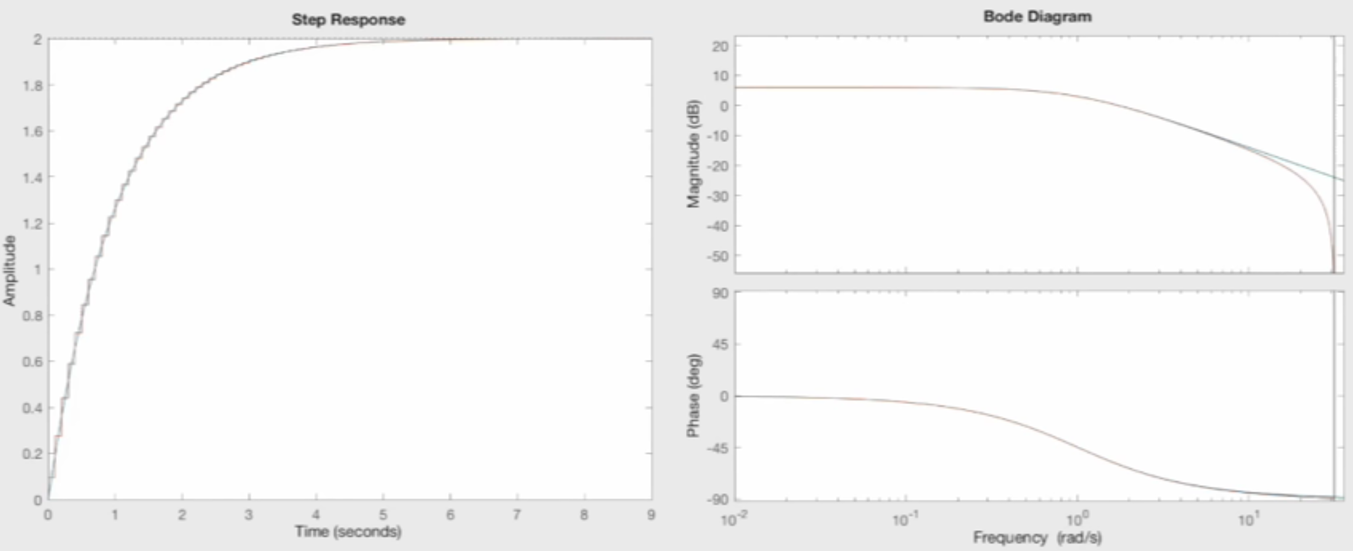
\includegraphics[width=1\textwidth]{Comparación de las respuestas, en el tiempo y en la frecuencia, de la función G(S) de ejemplo vs la función G(Z) obtenida utilizando el método de Tustin}
%     \caption{Comparación de las respuestas, en el tiempo y en la frecuencia, de la función G(S) de ejemplo vs la función G(Z) obtenida utilizando el método de Tustin.}
%     \label{fig:Comparación de las respuestas, en el tiempo y en la frecuencia, de la función G(S) de ejemplo vs la función G(Z) obtenida utilizando el método de Tustin}
% \end{figure}

% Como se puede observar, que el método de Tustin crea un sistema discreto que se comporta de forma muy similar a un sistema continuo, tanto en el dominio del tiempo como en el dominio de la frecuencia.

% La ecuación \ref{eq:Transformación Bilineal Inversa} se obtiene partiendo de la definición de la variable Z, la cual es:

% \begin{align}   \label{eq:Definición de Z}
%     Z=e^{S.T}
% \end{align}

% Debido a que dicha ecuación de Z en función de S \ref{eq:Definición de Z} es una función no lineal, no se utiliza como ecuación de transformación. Ya que (su transformación inversa) daría lugar a funciones de transferencia discretas G(Z) no lineales, por lo que no se podría mover cada polo y cero del dominio S al Z, y contruir G(Z) de forma fácil, solo se podría hacer para puntos individuales.

% Por ello, lo que se hace es linealizar $e^{S.T}$. Lo cual se puede lograr utilizando la siguiente expansión en serie de Taylor:

% \begin{align}   \label{eq:Expansión en Serie de Taylor para e^x}
%     e^x=\sum_{n=0}^{\infty}\frac{x^n}{n!}
% \end{align}

% La cual para $e^{S.T}$, se expande como:

% \begin{align}   \label{eq:Expansión en Serie de Taylor para e^(S.T)}
%     Z=e^{S.T}=1+\frac{S.T}{1}+\frac{\left(S.T\right)^2}{2}+\frac{\left(S.T\right)^3}{6}+...
% \end{align}

% De esta expasión, solo se toman los dos primeros términos para obtener la aproximación lineal de primer orden de Z:

% \begin{align}   \label{eq:Aproximación Lineal de Z}
%     Z \approx 1+S.T
% \end{align}

% Pero si se toma a $e^{S.T}$, se lo puede dividir en dos exponenciales como:

% \begin{align}   \label{eq:Artificio Matemático}
%     e^{S.T}=e^{\frac{S.T}{2}}.e^{\frac{S.T}{2}}=\frac{e^{\frac{S.T}{2}}}{e^{\frac{-S.T}{2}}}
% \end{align}

% Y tanto al numerador como al denominador se lo puede expandir como \ref{eq:Expansión en Serie de Taylor para e^(S.T)}, obteniendo:

% \begin{align}   \label{eq:Mejor Aproximación}
%     \frac{e^{\frac{S.T}{2}}}{e^{\frac{-S.T}{2}}}=\frac{1+\frac{S.T}{1}+\frac{\left(S.T\right)^2}{2}+\frac{\left(S.T\right)^3}{6}+...}{1-\frac{S.T}{1}+\frac{\left(S.T\right)^2}{2}-\frac{\left(S.T\right)^3}{6}+...}
% \end{align}

% Con lo que, tomando como aproximación solo los primeros dos términos de las series, se obtiene la ecuación \ref{eq:Transformación Bilineal Inversa} de la transformación bilineal inversa utilizada en el método de Tustin:

% \begin{align}   \label{eq:Transformación Bilineal Inversa Demostrada}
%     Z \approx \frac{1+\frac{S.T}{2}}{1-\frac{S.T}{2}}
% \end{align}

% La cual es una mejor aproximación de primer orden que \ref{eq:Aproximación Lineal de Z}.

% Cabe mencionar que cuando la constante de tiempo del sistema es lenta en comparación con los tiempos de muestreo, entonces todos los métodos de discretización producen respuestas prácticamente iguales, por lo que daría lo mismo cualquiere método. Pero, como se comentó, la idea es justamente tratar de utilizar un tiempo de muestreo lo más bajo posible, por lo que sí tiene importancia la elección de un método de discretización en particular.



\paragraph{DISCRETIZACIÓN DEL CONTROLADOR:}
\label{sec:DISCRETIZACIÓN DEL CONTROLADOR:}
\hfill

\hfill

Como se había comentado, el controlador completo consiste tanto del bloque controlador I-PD, como del bloque correspondiente al filtro de Kalman. Y ambos bloques son parte del software de la aplicación real, el cual se ejecuta sobre una computadora física. Por lo que, tanto el controlador I-PD propiamente dicho como el filtro de Kalman se implementan de forma discreta. Como ya se posee el filtro de Kalman implementado en forma discreta, se procede a discretizar el bloque controlador de simulink y luego ver los resultados del sistema completo, y analizar la estabilidad del mismo.

\begin{figure}[H]
    \centering
    \includegraphics[width=0.8\textwidth]{Parámetros del bloque del controlador P-ID discreto}
    \caption{Parámetros del bloque del controlador P-ID discreto.}
    \label{fig:Parámetros del bloque del controlador P-ID discreto}
\end{figure}


% EVALUACIÓN DE ESTABILIDAD DEL CONTROLADOR DISCRETO:
% - Luego de realizar la discretización del controlador se debe evaluar la estabilidad del sistema, ya que al ejecutar el controlador en una computadora (digital claro) se introducen retardos, debido a lo que se demora en ejecutar el algoritmo en cada iteración, lo que hace que en el diagrama de Bode se corra la curva de fase vs frecuencia hacia abajo, disminuyendo el margen de fase, lo que puede hacer que el sistema se vuelva inestable.

A continuación, se visualizan los bloques continuos y discretos del sistema completo:

\begin{figure}[H]
    \centering
    \includegraphics[width=1\textwidth]{Visualización de las bloques discretos y continuos del sistema}
    \caption{Visualización de las bloques discretos y continuos del sistema.}
    \label{fig:Visualización de las bloques discretos y continuos del sistema}
\end{figure}

Se puede observar que existen bloques fuera de la planta continua, que no son discretos; por lo que se procede a discretizarlos:

subparagraph{Discretización de la referencia de entrada al controlador I-PD:}
\label{sec:Discretización de la referencia de entrada al controlador I-PD:}
\hfill

La discretización de la consigna de posición, se logró cambiando el bloque integrador de la velocidad en el dominio S, por un bloque integrador en el dominio Z. El bloque signal builder con el que se genera la consigna trapezoidal de velocidad, no se pudo discretizar, probablemente por disponer de una versión vieja de MATLAB. Y sí debería ser discretizado en la implementación real.

\subparagraph{Discretización de la función S de nivel 2 de MATLAB:}
\label{sec:Discretización de la función S de nivel 2 de MATLAB:}
\hfill

Por otro lado, también se discretizó la función S de MATLAB de nivel 2, cambiando su parámetro de tiempo de muestreo, que determina la frecuencia con la que se llama a la función. Dicho parámetro se cambia en su código de MATLAB, en el setup, como se muestra a continuación:

\begin{figure}[H]
    \centering
    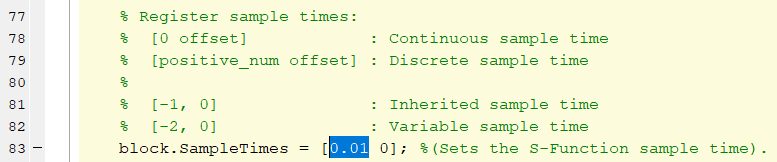
\includegraphics[width=0.7\textwidth]{Discretización de la función S de nivel 2 de MATLAB con T=0,01 s}
    \caption{Discretización de la función S de nivel 2 de MATLAB con T=0,01 s.}
    \label{fig:Discretización de la función S de nivel 2 de MATLAB con T=0,01 s}
\end{figure}

Como efecto colateral de discretizar esta función S de nivel 2, se obtiene una mejora en el tiempo de ejecución. Esto es, porque dicha función es el cuello de botella, por lo que al discretizarla se la está llamando menos veces en el tiempo. Y al hacer mayor el paso de tiempo T con el que se la llama, se obtiene una mejora en el tiempo de ejecución. Aunque claro, llega un valor de T en el que se comienza a ver demasiado discretizada la simulación en CoppeliaSim.

\begin{figure}[H]
    \centering
    \includegraphics[width=1\textwidth]{Revisualización de las bloques discretos y continuos del sistema}
    \caption{Revisualización de las bloques discretos y continuos del sistema.}
    \label{fig:Revisualización de las bloques discretos y continuos del sistema}
\end{figure}






%======================================================================
\section{RESULTADOS}
\label{sec:RESULTADOS}

Para el sistema completo, se obtiene la respuesta para tres valores del parámetro variable: su valor mínimo, su valor máximo, y un valor $J_l=6,2342 ~kg.m^2$, correspondiente a la posición articular [0,30,70,-50,120,0]°, el cual es un valor intermedio de los 4 puntos de operación tomados para el diseño de los respectivos 4 controladores I-PD:

\begin{figure}[H]
    \centering
    \includegraphics[width=1\textwidth]{Los tres puntos de operación evaluados}
    \caption{Los tres puntos de operación evaluados.}
    \label{fig:Los tres puntos de operación evaluados}
\end{figure}

\begin{figure}[H]
    \centering
    \includegraphics[width=1\textwidth]{Respuesta del sistema con filtro de Kalman}
    \caption{Respuesta del sistema con filtro de Kalman.}
    \label{fig:Respuesta del sistema con filtro de Kalman}
\end{figure}

Se observa que la posición angular $\theta_l$ estimada por el filtro de Kalman se corresponde perfectamente con la salida $\theta_l$ de la planta simulada. Incluso se corroboró que la salida $\theta_m$ estimada también sigue perfectamente a la $\theta_m$ de la planta simulada, y sin ruido notable.

\begin{figure}[H]
    \centering
    \includegraphics[width=1\textwidth]{Acercamiento a la respuesta del sistema con filtro de Kalman}
    \caption{Acercamiento a la respuesta del sistema con filtro de Kalman.}
    \label{fig:Acercamiento a la respuesta del sistema con filtro de Kalman}
\end{figure}

En este acercamiento se observa claramente, que aunque por más que $\theta_l$ estimada si describe un comportamiento deseado, las variables $v_a*$, $i_a$, y $\omega_l$ presentan un ruido mayor al ruido introducido al sistema. Esto es debido a que al momento de incorporar el filtro de Kalman al sistema, también se discretizó la familia de controladores I-PD. Con lo cual se obtiene una variable manipulada $v_a*$ discreta la cual produce las vibraciones en la corriente $i_a$, y por lo tanto también en la velocidad angular $\omega_l$. Esto produce pequeños sacudones en la velocidad del motor, los cuales describen una curva con una forma que depende fuertemente del paso de tiempo T del controlador discreto. Lo que ocurre es que la señal discreta va*[n], al entrar a la planta continua, simulink agrega (sin que lo veamos) un bloque de ZOH para convertir dicha señal discreta a una señal continua, la cual termina siendo una serie de escalones poco suavizados los cuales general ruido no deseado.

Por otro lado, se observa que para todos los valores del parámetro variable $J_l$ los valores de tensión y corriente se mantienen siempre dentro de los límites dados por la hoja de datos del motor; incluso con el ruido mencionado.

En las siguiente dos figuras se puede percibir que el seguimiento de consigna es adecuado.

\begin{figure}[H]
    \centering
    \includegraphics[width=1\textwidth]{Seguimiento de la consigna con filtro de Kalman para Jlmáx}
    \caption{Seguimiento de la consigna con filtro de Kalman para Jlmáx.}
    \label{fig:Seguimiento de la consigna con filtro de Kalman para Jlmáx}
\end{figure}

\begin{figure}[H]
    \centering
    \includegraphics[width=1\textwidth]{Respuesta a la perturbación con filtro de Kalman para Jlmáx}
    \caption{Respuesta a la perturbación con filtro de Kalman para Jlmáx.}
    \label{fig:Respuesta a la perturbación con filtro de Kalman para Jlmáx}
\end{figure}

% ======================================================================
\section{CONCLUSIONES}
\label{sec:CONCLUSIONES}

Se concluye que en forma general se cumplieron los objetivos del proyecto, en el desarrollo del sistema de control de posición para el accionamiento electromecánico de la primer articulación del robot Universal UR10. Se modeló correctamente el sistema LTI en el espacio de estados, y se pudo aplicar la técnica de planificación de ganancias, obteniendo una familia de controladores I-PD, que lograron proporcionar un correcto seguimiento de consignas y rechazo de perturbaciones.

Luego, se incorporó ruido en el proceso, y en el sensado de la posición, y luego se utiliza el filtro de Kalman con el objetivo de mitigar dichos ruidos. El filtro de Kalman se lo implentó en tiempo discreto, y con ello también se discretizó el controlador de forma exitosa. Con lo que también se logró un excelente seguimiento de la consigna y reachzo de perturbaciones, e incluso con una variable manipulada discreta la cual introduce un ruido importante en el sistema.

Con lo que terminó obteniendo un buen control de la planta, aunque el proyecto puede ser mejorado en varios aspectos como se indica a continuación.

\subsection{Mejoras}
\label{sec:Mejoras}

\paragraph{RUIDO INTRODUCIDO POR LA SEÑAL MANIPULADO DISCRETA:}
\label{sec:RUIDO INTRODUCIDO POR LA SEÑAL MANIPULADO DISCRETA:}
\hfill

Como principal mejora, se debería mitigar el ruido provocado por la salida discreta del controlador I-PD. Ya que provoca un ruido no deseado en las variables de estado de la planta, el cual es mayor al propio ruido de proceso introducido para simular las incertidumbres del modelo. Para ello se debería implementar un filtro pasa bajos a la salida del controlador discreto, el cual permita atenuar las componentes de alta frecuencia generadas por la señal cuadrada $v_a*(t)$. Se propone la implementación de un filtro gigital del tipo FIR, el cual en comparación con el filtro IIR, el \textbf{Filtro FIR}:

\begin{description}
    \item[-] Tiene una respuesta al impulso finita, lo que significa que su salida depende solo de un número finito de entradas anteriores.
    \item[-] Es fácil de diseñar e implementar.
    \item[-] Tiende a ser más estable y menos propenso a problemas de inestabilidad.
    \item[-] No involucra retroalimentación, lo que lo hace más adecuado para ciertas aplicaciones.
\end{description}



\paragraph{ERROR DE ESTADO ESTACIONARIO EN RAMPA:}
\label{sec:ERROR DE ESTADO ESTACIONARIO EN RAMPA:}
\hfill

En las respuestas del sistema se observó cierto valor de error de estado estacionario al describirse una rampa. Y, aunque luego se termina corrigiendo rápidamente, durante la rampa se obtiene en cada instante una diferencia 27° entre el valor de refencia y la posición angular del robot en la simulación. Dicho error es posible mitigarlo y se propone como mejora.

\paragraph{REPRESENTACIÓN EN PUNTO FIJO:}
\label{sec:REPRESENTACIÓN EN PUNTO FIJO:}
\hfill

El controlador final obtenido es completamente discreto. El cual, en la aplicación correrá en un hardware digital. En el cual los números se almacenan en palabras binarias, es decir secuencias de bits (unos y ceros). Y la forma en que los componentes de hardware y las funciones de software interpretan esta secuencia de unos y ceros, viene definida por el tipo de datos. Se tiene que los números binarios se representan como tipos de datos de punto fijo o de punto flotante.

Si bien la representación en punto fijo posee una menor precisión que la representación en punto flotante, los cálculos en punto fijo generalmente son más rápidos y consumen menos recursos que los cálculos en punto flotante, lo que los hace más adecuados para sistemas con restricciones de tiempo real, colo lo es la aplicación del presente proyecto. Además, la implementación en hardware de operaciones en punto fijo es generalmente más simple y eficiente, lo que la hace más atractiva para dispositivos embebidos y sistemas integrados.

Por lo que, para la aplicación, se elige la representación en punto fijo.

Dicho esto, entonces queda como mejora el generar un código eficiente representado en punto fijo a partir del modelo obtenido. Y también, simular el comportamiento matemático del hardware del ordenador. Para lo cual se propone, utilizar la herramienta de Fixed-Point Designer de MathWorks, el cual permite controlar los tipos de datos numéricos de las señales y sus parámetros, y optimizar el código, entre otras funcionalidades.


\paragraph{EFECTOR FINAL:}
\label{sec:EFECTOR FINAL:}
\hfill

Una vez definida una aplicación en específico, se puede mejorar la prueba monoarticular del robot, al agregarle un efector final al mismo, y una carga (si es que se correspondee con el tipo de efector final). Por ejemplo, podría ser una aplicación de pick and place para la alimentación de una máquina CNC, en donde se tendría una pinza robótica (en inglés: gripper) o bien una ventosa de vacío, para agarrar por ejemplo una pieza metálica de forma cilindrica a ser mecanizada. En tal caso, simplemente se debería incluir las masas, y momentos y productos de inercia del gripper y de la pieza a mover, en el cálculo del momento de inercia $J_Z$ de la primer articulación. Y como aumentaría el valor de dicho momento de inercia entonces además requeriría agregar más puntos de operación al aplicar el método de gain scheduling, para contemplar los mayores valores del parámetro variable.


\paragraph{CONTROL MONOARTICULAR DE CUALQUIER ARTICULACIÓN:}
\label{sec:CONTROL MONOARTICULAR DE CUALQUIER ARTICULACIÓN:}
\hfill

Por otro lado, aunque el proyecto se centró en realizar el control monoarticular de solo la primer articulación del robot, el control monoarticular de otra de sus articulaciones es relativamente similar. La mayor diferencia radica en el modelo mecánico, ya que en las demás articulaciones sí habría que incluir la gravedad a la hora de formular su modelo mecánico; debido a que cuando una articulación no posee su eje de giro siempre paralelo a la dirección de la aceleración de la gravedad, entonces esta sí influye en su movimiento. Además, el cálculo del momento de inercia equivalente se vería modificado. Y, con dichos cambios se verían obviamente modificados también los valores de las ganancias de la familia de controladores PID.








% ======================================================================
\section*{Bibliografía}

Wikibooks. Online \LaTeX{} book.
\href{https://en.wikibooks.org/wiki/LaTeX/}{URL}.

Overleaf. Learn LaTeX in 30 minutes.
\href{https://www.overleaf.com/learn/latex/Learn_LaTeX_in_30_minutes}{URL}.

Overleaf. Bibliography management in LaTeX.
\href{https://www.overleaf.com/learn/latex/Bibliography_management_in_LaTeX}{URL}.

Real Academia Española, Tecnicismos, neologismos y extranjerismos en el español.
\href{http://revistas.rae.es/bilrae/article/view/218/525}{URL}.

Rodrigo Gonzalez. Guía para la redacción del proyecto final de Control y Sistemas.
\href{https://es.overleaf.com/project/5ce7209e973f0d6ead24dcef}{URL}.

Rodrigo Gonzalez. Filminas de clase. Control y Sistemas. UNCuyo.
\href{https://github.com/rodralez/control}{URL}.

Simscape: model and simulate multidomain physical systems. The MathWorks, Inc.
\href{https://la.mathworks.com/products/simscape.html}{URL}.

Manual de CoppeliaSim.
\href{https://manual.coppeliarobotics.com/}{URL}.

Universal Robots Forum.
\href{https://forum.universal-robots.com/}{URL}.

Franco Bizzotto. Proyecto: Modelado y diseño de controlador para robot serie redundante.
\href{https://github.com/carloshernangarrido/control/blob/master/12_anteproyecto_proyecto-final/Bizzotto_Robot-serie.pdf}{URL}.

Ogata. Diseño de control moderno. 5ta edición. Pearson.

Krishnan R ELECTRIC MOTOR DRIVES - Modeling Analysis and Control Prentice Hall 2001

Lyons. Understanding Digital Signal Processing. 3ra edición, Prentice Hall



% ======================================================================
\printbibliography%[heading=bibintoc] %(Descomentar esto último de esta línea para que aparezcan las referencias en el índice).


% ======================================================================
\section*{Apéndice}
% Material adicional que es importante agregar para dar un acabado entendimiento del reporte. Por ejemplo, código fuente, planos mecánicos o especificaciones de sensores.

\paragraph*{Función S de nivel 2 de MATLAB}
\label{sec:Función S de nivel 2 de MATLAB}
\hfill

\inputminted{matlab}{SIMULACION_CoppeliaSim.m}


\subsubsection*{Código fuente en MATLAB:}
\label{sec:Código fuente en MATLAB:}
\hfill

\inputminted{matlab}{Codigo.m}






\end{sloppypar}
\end{document}
